%%% LaTeX Template
%%% This template can be used for both articles and reports.
%%%
%%% Copyright: http://www.howtotex.com/
%%% Date: February 2011

%%% Preamble
\documentclass[paper=a4, fontsize=9pt]{scrartcl}	% Article class of KOMA-script with 11pt font and a4 format

\usepackage[english]{babel}															% English language/hyphenation
\usepackage[protrusion=true,expansion=true]{microtype}	% Better typography
\usepackage{amsmath,amsfonts,amsthm,commath,mathtools} % Math packages

\usepackage[pdftex]{graphicx}														% Enable pdflatex
\graphicspath{{img/}}
%\usepackage{color,transparent}													% If you use color and/or transparency
\usepackage[hang, small,labelfont=bf,up,textfont=it,up]{caption}	% Custom captions under/above floats
\usepackage{epstopdf}																	% Converts .eps to .pdf
\usepackage{subfig}																		% Subfigures
\usepackage{booktabs}																	% Nicer tables


%%% Advanced verbatim environment
\usepackage{verbatim}
\usepackage{fancyvrb}
\DefineShortVerb{\|}								% delimiter to display inline verbatim text


%%% Custom sectioning (sectsty package)
\usepackage{sectsty}								% Custom sectioning (see below)
\allsectionsfont{%									% Change font of al section commands
	\usefont{OT1}{bch}{b}{n}%					% bch-b-n: CharterBT-Bold font
%	\hspace{15pt}%									% Uncomment for indentation
	}

\sectionfont{%										% Change font of \section command
	\usefont{OT1}{bch}{b}{n}%					% bch-b-n: CharterBT-Bold font
	\sectionrule{0pt}{0pt}{-5pt}{0.8pt}%	% Horizontal rule below section
	}


%%% Custom headers/footers (fancyhdr package)
\usepackage{fancyhdr}
\pagestyle{fancyplain}
\fancyhead{}														% No page header
\fancyfoot[C]{\thepage}										% Pagenumbering at center of footer
%\fancyfoot[R]{\small \texttt{HowToTeX.com}}	% You can remove/edit this line 
\renewcommand{\headrulewidth}{0pt}				% Remove header underlines
\renewcommand{\footrulewidth}{0pt}				% Remove footer underlines
\setlength{\headheight}{13.6pt}

%%% Equation and float numbering
\numberwithin{equation}{section}															% Equationnumbering: section.eq#
\numberwithin{figure}{section}																% Figurenumbering: section.fig#
\numberwithin{table}{section}																% Tablenumbering: section.tab#


%% IRINA's STUFF
\setlength{\parindent}{4em}
\setlength{\parskip}{1em}
\renewcommand{\baselinestretch}{1.0}

\usepackage{color}
\usepackage[dvipsnames]{xcolor}
\usepackage{parskip}
\usepackage{enumerate}
\usepackage{float}
\usepackage{multicol}
\usepackage[export]{adjustbox}
\usepackage[left=1.5cm, right=1.5cm, top=1.5cm, bottom=2.0cm]{geometry}
\usepackage{listings}
\usepackage{wrapfig}
\usepackage[framed,numbered,autolinebreaks,useliterate]{mcode}
\usepackage{cancel}
\usepackage{amsmath}
\usepackage{hyperref}
\usepackage{csquotes}
\usepackage{mdframed}
\usepackage{wrapfig}
\usepackage{longtable}



%% IRINA'S COMMANDS
\newcommand{\gammabar}{\ensuremath\gamma\kern-0.65em-}


\newcommand\courtesy{[Image courtesy of Haacke et al. \textit{Magnetic Resonance Imaging: Physical Principles and Sequence Design, volume 1st.  Wiley-Liss, 1999} \cite{Haacke1999}]}

\newcommand\courtesyText{[Quotation courtesy of Haacke et al. \textit{Magnetic Resonance Imaging: Physical Principles and Sequence Design, volume 1st.  Wiley-Liss, 1999} \cite{Haacke1999}]}

\newcommand\courtesywiki{[Image courtesy of \href{https://en.wikipedia.org}{Wikipedia}]}




\usepackage{array}

\newenvironment{conditions}
  {\par\vspace{\abovedisplayskip}\noindent\begin{tabular}{>{$}l<{$} @{${}={}$} l}}
        {\end{tabular}\par\vspace{\belowdisplayskip}}

%%% Title	
\title{ \vspace{-1in} 	\usefont{OT1}{bch}{b}{n}
		\huge \strut Magnetic Resonance Imaging \strut \\
		\Large \bfseries \strut Physical Principles and Sequence Design \strut
}
\author{\usefont{OT1}{bch}{m}{n}
        Irina Grigorescu \\		\usefont{OT1}{bch}{m}{n}
        UCL\\	\usefont{OT1}{bch}{m}{n}
        \texttt{irina.grigorescu.15@ucl.ac.uk}
}
\date{}

%%% Begin document
\begin{document}
\maketitle
\tableofcontents

%%%%%%%%%%%%%%%%%%%%%%%%%%%%%%
%% CHAPTER 1
%%%%%%%%%%%%%%%%%%%%%%%%%%%%%%
\newpage
\section{Magnetic Resonance Imaging: A Preview}

\subsection{Summary}
\begin{enumerate}
    \item The name \textbf{MRI}
    \begin{itemize}
        \item \textbf{M}agnetic - the use of magnetic fields in the field
        \item \textbf{R}esonance - the need to match the frequency of an oscillating magnetic field to the precessional frequency of the spins of some nucleus
        \item \textbf{I}maging
    \end{itemize}

    \item \textbf{MRI} Concepts
    \begin{itemize}
        \item Based on the \textit{interaction of a nuclear spin with an external magnetic field $\vec{B_0}$}
        \item Precession - \textit{the circular motion of the axis of rotation of a spinning body about another fixed axis caused by the application of a torque in the direction of the precession}
        \item Imaging - based on the \textit{bulk precession of the hydrogen spins about the field direction} (Figure~\ref{fig:fig11})
        \item Precession angular frequency (Larmor Equation): \\
            \begin{equation} 
                \omega_0 = \gamma B_0
            \end{equation}

            where:
            \begin{conditions}
                \gamma & gyromagnetic ratio ($2.68 \times 10^8 rad/s/tesla$)
            \end{conditions}

        \item The Boltzmann Distribution shows that the spins can align both parallel and antiparallel with to the magnetic field. The spin excess is very small: \\
            \begin{equation} 
                \text{spin excess } \simeq N \frac{\hbar \omega_0}{2kT}
            \end{equation}

            where:
            \begin{conditions}
                N & total number of spins present in the sample \\
                k & Boltzmann constant \\
                kT & average thermal energy 
            \end{conditions}

        \item $M_0$ - the average magnetic dipole density (longitudinal equilibrium relaxation)
            \begin{equation}
                M_0 = \frac{\rho_0 \gamma^2 \hbar^2}{4kT} B_0
            \end{equation}
           
        \item $\vec{M}$ has been rotated by an rf pulse to a direction orthogonal to $\vec{B_0} = B_0 \hat{z}$. The resulting transvserse magnetization has magnitude $M_0$ and precesses clockwise in the x-y plane. The complex magnetization is:
            \begin{equation}
                M_+(t) \equiv M_x(t) + i M_y(t) = M_0 e^{-i \omega t + i \phi_0}
            \end{equation}
    \end{itemize}
\end{enumerate}

\begin{figure}[H]
	\centering
	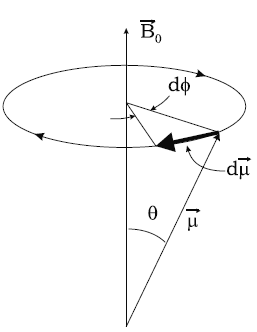
\includegraphics[width=0.4\textwidth,keepaspectratio]{fig11}
	\caption{
By definition, precession is the circular motion of the axis of rotation of a spinning body
about another fixed axis caused by the application of a torque in the direction of the precession.
The interaction of the proton's spin with the magnetic field produces the torque, causing it to
precess about $\vec{B_0}$ as the fixed axis. When looking down from above the vector $\vec{B_0}$, the precession
of the magnetic moment vector $\vec{\mu}$, which is proportional to the spin vector, is clockwise. For the
customary counterclockwise definition of polar angles, the differential $d\phi$ shown is negative.}
	\label{fig:fig11}
\end{figure}

\begin{figure}[H]
	\centering
	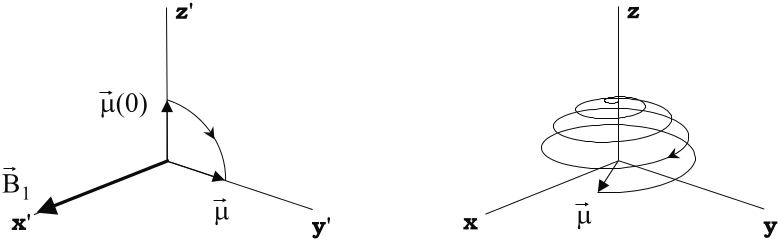
\includegraphics[width=0.7\textwidth,keepaspectratio]{fig12}
	\caption{
Illustration of the effect of an rf pulse on an individual magnetic moment $\mu$. \\
(a) In a frame rotating about $B_0$ (which is along $\hat{z}$, say) at the Larmor frequency (with coordinates
x', y' and z' = z), there is no observed precession about $B_0$. Upon application of an rf magnetic
field pulse applied along $\hat{x}'$, the magnetic moment is rotated about $\hat{x}'$ at a rate corresponding to
the frequency $\omega_1 = \gamma B_1$ determined by the amplitude of the rf field, $B_1$. A $\pi/2$ flip
relative to its starting position along $\hat{z}'$ is achieved in a 
time $\tau_{rf}$ provided that $\omega_1 \tau_{rf} = \pi/2$.\\
(b) The behavior of the same magnetic moment rotation is observed to be more complicated in the fixed laboratory
frame. This picture has been constructed for the case $\omega_1 = 0.06 \omega_0$. In actual MR applications, the
frequency $\omega_1$ would be much smaller in relation to $\omega_0$, but then the spiraling would be too dense
to illustrate.
}
	\label{fig:fig12}
\end{figure}

\begin{figure}[H]
	\centering
	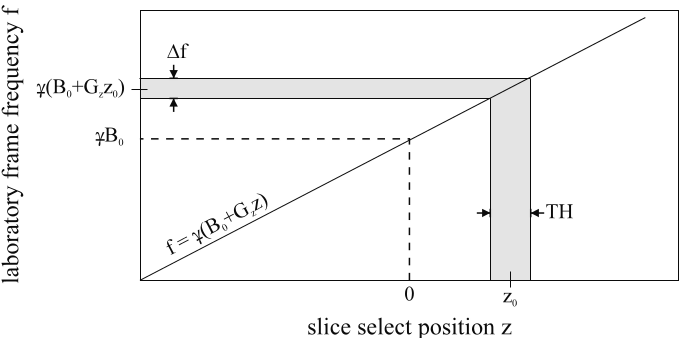
\includegraphics[width=0.7\textwidth,keepaspectratio]{fig13}
	\caption{
The precession frequency ($f = \omega/(2\pi)$) in the laboratory frame is a function of position
along the slice select axis. The original static field $B_0$ has been supplemented with a field with
constant gradient $G_z$ in the z-direction. The central frequency and spectral bandwidth of the rf
pulse ($\Delta f \equiv BW_{rf}$, the shaded horizontal strip) are such that the slice of thickness 
$\Delta z \equiv T H$ (the
shaded vertical strip) is uniformly 'excited' (i.e., all spins in the slice have the resonance condition
satisfied). The fact that the slice is offset from the origin in the z-direction by $z_0$ implies that the
center frequency of the rf pulse must be offset from the static Larmor frequency $f_0 = \gammabar B_0$ by $\gammabar G_z z_0$ as has been shown along the frequency axis. }
	\label{fig:fig13}
\end{figure}

\begin{figure}[H]
	\centering
	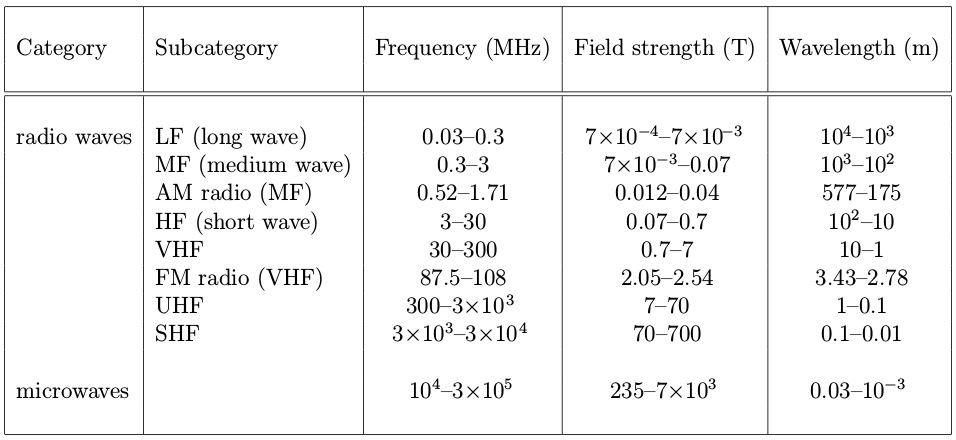
\includegraphics[width=0.8\textwidth,keepaspectratio]{tab11}
	\caption{
Range of radio and microwave frequencies from Wikipedia at en.wikipedia.org. Under
the subcategory heading, the letter F refers to frequency. The letters L, M, H, V, U, and S in front
of the letter F refer to low, medium, high, very, ultra, and super, respectively. Associated free-space
wavelengths and NMR field strengths for protons are given here.
}
	\label{fig:tab11}
\end{figure}

\clearpage
%%%%%%%%%%%%%%%%%%%%%%%%%%%%%%
%% EXERCISES
\newpage
\subsection{Exercises}

%%%%%%%%%%%%%%%%%%%%%%%%%%%%%%
\Large{Problem 1.1}
\begin{figure}[H]
    \centering
    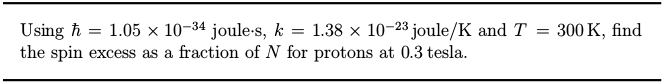
\includegraphics[width=0.8\textwidth,keepaspectratio]{prbl11}
    \label{fig:prbl11}
\end{figure}

\textit{Remember:}
\begin{itemize}
	\item This problem shows how to calculate the excess amount of spins occupying a lower energy level relative to the higher energy level, in a sample immersed in a static magnetic field.
\end{itemize}

\lstinputlisting{../project/functions/ch1/excessSpins.m}

\clearpage

\Large{Problem 1.2}
\begin{figure}[H]
    \centering
    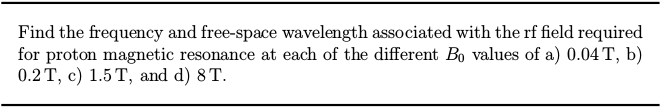
\includegraphics[width=0.8\textwidth,keepaspectratio]{prbl12}
    \label{fig:prbl12}
\end{figure}

\textit{Remember:}
\begin{itemize}
	\item This problem computes the resonance frequency of the oscillating magnetic field for a given static polarising magnetic field.
\end{itemize}

\lstinputlisting{../project/functions/ch1/resonanceFrequency.m}

\textit{Remember: (For the opposite problem)}
\begin{itemize}
	\item This problem computes the field strength associated with the frequency of an RF field for a given gyromagnetic ratio.
\end{itemize}

\lstinputlisting{../project/functions/ch1/fieldStrength.m}


\clearpage

%%%%%%%%%%%%%%%%%%%%%%%%%%%%%%
%% CHAPTER 2
%%%%%%%%%%%%%%%%%%%%%%%%%%%%%%
\newpage
\section{Classical Response of a Single Nucleus to a Magnetic Field}

\subsection{Summary} 
\begin{enumerate}
    \item This chapter investigates a single proton's response to an external magnetic field.
    \item The magnetic moment of the spin in the presence of an external magnetic field will align with the external field as this is its equilibrium state.

    \begin{itemize}
        \item A current loop of current $I$ (and area $A$) placed in an external magnetic field $B$ will experience a differential force on the loop determined by the cross product between the differential current and the magnetic field. \\
        \begin{equation}
            d\vec{F} = I d\vec{l} \times \vec{B}
        \end{equation}

        \item The total force on this loop (or any closed loop) will be zero. This can be derived by taking the integral over the equation above. This leads to a zero change in the total momentum $p$ as: \\
        \begin{equation}
            \vec{F} = \frac{d\vec{p}}{dt}
        \end{equation}

        \item In conclusion, a current loop found at rest in a constant external magnetic field 
        will remain at rest unless external forces are applied, 
        depending on the orientation (like in Figure~\ref{fig:fig21}a). 
        Otherwise, they will experience a torque which will rotate the loop.
        \begin{figure}[H]
            \centering
            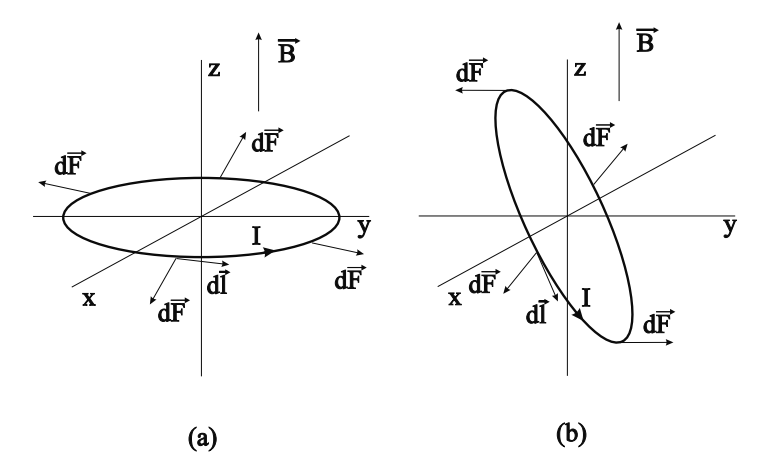
\includegraphics[width=0.6\textwidth,keepaspectratio]{fig21}
            \caption{
           Circular current loop depicted in two different orientations relative to a uniform magnetic
        field. The forces on representative differential current segments are shown (one \textit{d} is explicitly shown
        in each case). The first (a) shows the current plane perpendicular to the field where there is no
        net twist (torque); the second (b) shows the current plane at an arbitrary angle to the field where
        there is a nonzero torque. 
            }
            \label{fig:fig21}
        \end{figure}

        \item In other words, if the current loop is not at rest, then it will try to rotate itself to be at rest. Rotations can also arise from forces applied off-centre even when the sum of all differential forces is zero. Rotations are described by a force called \textbf{torque}. Each differential segment experiences a differential torque: \\
        \begin{equation}
            d\vec{N} = \vec{r} \times d\vec{F}
        \end{equation}

        \item The total sum of these differential torques is zero for non-rotating objects, and nonzero for rotating ones. This is exemplified in Figure~\ref{fig:fig21} and in Exercises \ref{fig:ex21} and \ref{fig:ex22}.

        \item For any arbitrary current distribution, the net torque has the following formula: \\
        \begin{equation} \label{eq:eq24}
            \vec{N} = \vec{\mu} \times \vec{B}
        \end{equation}
        where $\vec{\mu}$ is called the magnetic dipole moment or magnetic moment. 
        
        \item The magnetic moment vector for planar loops is given in
            terms of the current going through the loop \textit{I}, the area of the
            loop \textit{A} and the unit vector $\vec{n}$ perpendicular to the
            current loop plane \\
        \begin{equation} \label{eq:eq25}
            \vec{\mu} = I A \hat{n}
        \end{equation}
        This can be visualised in Figure~\ref{fig:fig22}.
        \begin{figure}[H]
            \centering
            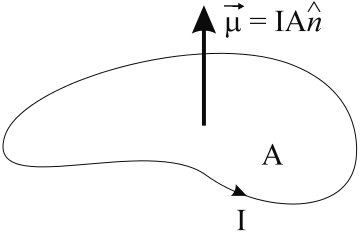
\includegraphics[width=0.4\textwidth,keepaspectratio]{fig22}
            \caption{ A loop with current I lying in a plane
            } 
            \label{fig:fig22}
        \end{figure}
        
        
        \item An example \\
            For Figure~\ref{fig:fig23a}, 
            the total torque for planar loops will depend on the current
            \textit{I} (anticlockwise), the magnetic field strength \textit{B}, the angle
            \textit{$\theta$} between the plane in which the current loop lies and the
            magnetic field and the total area of the loop. \\ 
        
        To get to this we begin with: 
        \begin{align}
            d\vec{N} = \vec{r} \times (Id\vec{l} \times \vec{B}) = Id\vec{l}(\vec{B} \cdot \vec{r}) - I \vec{B} (d\vec{l} \cdot \vec{r})
        \end{align}
        where $\vec{B}$ and the cylindrical unit vectors looking like:
        
        \begin{align}
            \vec{B} = B(cos \theta \text{ } \hat{z} + sin \theta \text{ } \hat{y}) \\
            \hat{\rho} = cos \phi \text{ } \hat{x} + sin \phi \text{ } \hat{y} \\
            \hat{\phi} = - sin \phi \text{ } \hat{x} + cos \phi \text{ } \hat{y}
        \end{align}
        
        Calculating and integrating over we arrive at:
        \begin{equation} \label{eq:eq29}
            \vec{N} = − I \pi R 2 B sin\theta \hat{x}
        \end{equation}

        \begin{figure}[H]
            \centering
            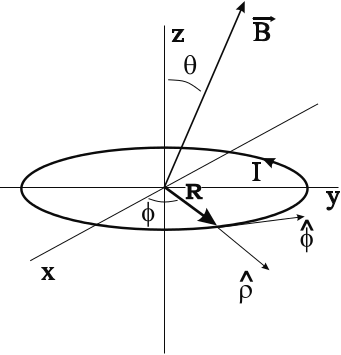
\includegraphics[width=0.4\textwidth,keepaspectratio]{fig23a}
            \caption{ A circular loop in x-y plane and the magnetic field lying in the y-z plane
            } 
            \label{fig:fig23a}
        \end{figure}

    \end{itemize}

    \item Spin has intrinsic angular momentum. Magnetic moment is proportional to it. In this case the motion is changed.
    \begin{itemize}
        \item In the picture painted so far we introduce 'spinning', or \textbf{angular momentum}.

        \begin{itemize}
            \item The change in the angular momentum of the spin will equal torque.
            \begin{equation} \label{eq:eq214}
                \frac{d\vec{J}}{dt} = \vec{N}
            \end{equation}
            
            \item This comes from (a system of many point particles with respect to some origin):
            \begin{equation} \label{eq:eq215}
                \vec{J} = \sum_i \vec{r}_i \times \vec{p}_i
            \end{equation}
            where $d\vec{p} = \vec{F} dt$
            
            \textcolor{gray}{\textbf{Sidenote}: \\
            $\vec{p}$ is linear momentum \\
            $\vec{r} \times \vec{p}$ is angular momentum    
            }
        \end{itemize}

        \item There exists a connection between intrinsic angular momentum and its moment
        \begin{itemize}
            \item The direct relationship between the magnetic moment and
            the spin angular momentum vector is found from experiment:
            \begin{equation} \label{eq:eq216}
                \vec{\mu} = \gamma \vec{J}
            \end{equation}

            where $\gamma$ is called the \textit{gyromagnetic ratio} and it depends on the particle or nucleus. For the proton nucleus it is: 
            \begin{equation} 
                \gamma = 2.675 \times 10^8 \text{rad/s/T}
            \end{equation}            
        \end{itemize}        

        \item The equation of motion of a precessing spin immersed in a static polarising magnetic field can be found using Eq~\ref{eq:eq216} and Eq~\ref{eq:eq24} in Eq~\ref{eq:eq214} (also known as a simple version of the Bloch equation):
        \begin{equation} \label{eq:eq224}
            \frac{d\vec{\mu}}{dt} = \gamma \vec{\mu} \times \vec{B}
        \end{equation}

    \end{itemize}

    \item Geometrical Representation
    \begin{multicols}{2}
    \begin{align*}
        R = \abs{\mu} \cdot sin\theta \\
        d\vec{\mu} = R \cdot \abs{d\phi} \\
        d\vec{\mu} = \abs{\vec{\mu}} \cdot sin\theta \cdot \abs{d\phi}
    \end{align*}

    \vfill
    \columnbreak

    \begin{figure}[H]
        \centering
        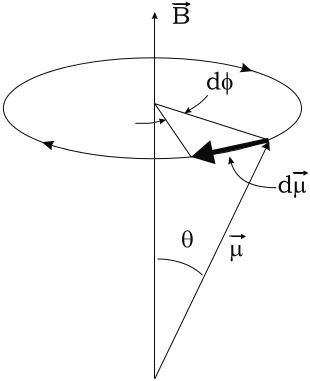
\includegraphics[width=0.3\textwidth,keepaspectratio]{fig25}
        \caption{ Clockwise precession of a proton's spin about a magnetic field.
        } 
        \label{fig:fig25}
    \end{figure}

    \end{multicols}

    \begin{equation}\label{eq:eq225}
        \abs{d\vec{\mu}} = \mu\, sin\theta\, \abs{d\phi}
    \end{equation}
    From Eq~\ref{eq:eq224}:
    \begin{equation}\label{eq:eq226}
        \abs{d\vec{\mu}} = \gamma \abs{\vec{\mu} \times \vec{B}} dt = \gamma\, \mu\, B\, sin \theta\, dt
    \end{equation}
    From Eq~\ref{eq:eq225} and ~\ref{eq:eq226} we have: $\abs{d\phi} = \gamma\, B\,dt$.\\
    Because $\omega = \abs{\frac{d\phi}{dt}}$, we get the famous Larmor precession formula:
    \begin{equation}\label{eq:eq227}
        \omega = \gamma\, B
    \end{equation}
    Also, because we have a clockwise rotation in the figure:
    \begin{equation}\label{eq:eq228}
        \frac{d\phi}{dt} = - \omega
    \end{equation}
    If the field is along the z-axis and constant in time, $\vec{B} = B_0 \hat{z}$,
    the solution for Eq~\ref{eq:eq228} is:
    \begin{equation}\label{eq:eq230}
        \phi = - \omega_0 t + \phi_0
    \end{equation}

    %%%%%%%%%%%%%%%%%%%%%%%%%%%%%%%%%%%%%%%%%%
    \item Cartesian Representation
    \begin{multicols}{2}
    \begin{align*}
        \vec{\mu_x}(t) = \vec{\mu}(t) \cdot cos(\phi_0 - \xi) \\
        \vec{\mu_x}(t) = \vec{\mu}(t) \cdot (cos \phi_0 \cdot cos \xi + sin \phi_0 \cdot sin \xi ) \\
        \vec{\mu_x}(t) = \vec{\mu}(t) \cdot cos \phi_0 \cdot cos \xi \\
        + \vec{\mu}(t) \cdot sin \phi_0 \cdot sin \xi  \\
        \vec{\mu_x}(t) = \vec{\mu}(t) \cdot \frac{\vec{\mu_x}(0)}{\vec{\mu}(0)} \cdot cos \xi \\
        + \vec{\mu}(t) \cdot  \frac{\vec{\mu_y}(0)}{\vec{\mu}(0)} \cdot sin \xi  \\
        \vec{\mu_x}(t) = \vec{\mu_x}(0) \cdot cos \xi + \vec{\mu_y}(0) \cdot sin \xi \\
    \end{align*}

    \vfill
    \columnbreak

    \begin{figure}[H]
        \centering
        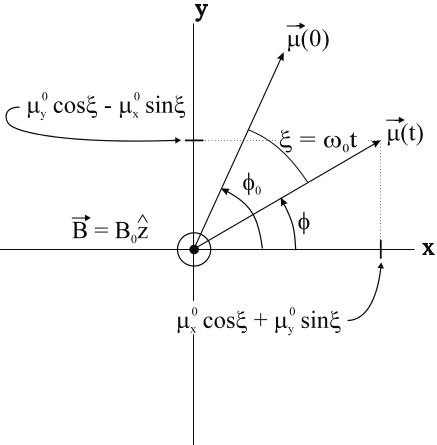
\includegraphics[width=0.4\textwidth,keepaspectratio]{fig26a}
        \caption{ } 
        \label{fig:fig26a}
    \end{figure}

    \end{multicols}

    For $\vec{B} = B_0 \hat{z}$ we have:
    \begin{equation}\label{eq:eq232}
        \vec{\mu}(t) = \vec{\mu_x}(t)\hat{x} + \vec{\mu_y}(t)\hat{y} +  \vec{\mu_z}(t)\hat{z}
    \end{equation}
    with:
    \begin{align}\label{eq:eq233}
        {\mu_x}(t) = {\mu_x}(0) \cdot cos \omega_0 t + {\mu_y}(0) \cdot sin \omega_0 t \\
        {\mu_y}(t) = {\mu_y}(0) \cdot cos \omega_0 t - {\mu_x}(0) \cdot sin \omega_0 t \\
        {\mu_z}(t) = {\mu_z}(0)
    \end{align}

    %%%%%%%%%%%%%%%%%%%%%%%%%%%%%%%%%%%%%%%%%%
    \item Matrix Representation
    \begin{equation}\label{eq:eq236}
        \vec{\mu}(t) = R_z(\omega_0t) \vec{\mu}(0)
    \end{equation}
    with:
    \begin{equation}
    R_z(\theta)=
    \begin{pmatrix}
    cos\theta & sin\theta & 0 \\
    -sin\theta & cos\theta & 0 \\
    0 & 0 & 1
    \end{pmatrix}
    \end{equation}

    %%%%%%%%%%%%%%%%%%%%%%%%%%%%%%%%%%%%%%%%%%
    \item Complex Representation and Phase
    The two degrees of freedom, ${\mu_x}$ and ${\mu_y}$, can be given in terms of the real and
    imaginary parts of:
    \begin{equation}
        {\mu_{+}}(t) = {\mu_x}(t) + i {\mu_y}(t)
    \end{equation}
    with:
    \begin{equation}
        {\mu_{+}}(t) = {\mu_{+}}(0) e^{-i\omega_0t}
    \end{equation}

    In general, the complex number ${\mu_{+}}(t)$ can be written in terms of its magnitude and phase:
    \begin{equation}
        {\mu_{+}}(t) = \abs{{\mu_{+}}(t)} e^{i\phi (t)}
    \end{equation}
    So, the complex representation can be rewritten as:
    \begin{equation}
        {\mu_{+}}(t) = \abs{{\mu_{+}}(0)} e^{i\phi_0 (t)}
    \end{equation}
    where the phase is:
    \begin{equation}
        \phi_0(t) = -\omega_0 t + \phi_0(0)
    \end{equation}

\end{enumerate}

\clearpage

%%%%%%%%%%%%%%%%%%
% \clearpage
%%%%%%%%%%%%%%%%%%%%%%%%%%%%%%%%%%%%%%%%%%
% \subsection{Magnetic Moment in the Presence of a Magnetic Field}
% \begin{itemize}
%     \item This section reviews Physics concepts such as: magnetic force, magnetic moment given by a current loop, torque due to force and torque’s relation to the magnetic moment and the magnetic field.
% \end{itemize}

% \subsubsection{Torque on a Current Loop in a Magnetic Field}
% \begin{itemize}
%     \item Placing a current loop of current $I$ (and area $A$) in an external magnetic field $B$ will create a differential force on the loop determined by the cross product between the differential current and the magnetic field. \\
%     \begin{equation}
%         d\vec{F} = I d\vec{l} \times \vec{B}
%     \end{equation}

%     \item The total force on this loop (or any closed loop) will be zero. This can be derived by taking the integral over the equation above. This leads to a zero change in the total momentum $p$ as: \\
%     \begin{equation}
%         \vec{F} = \frac{d\vec{p}}{dt}
%     \end{equation}

%     \item In conclusion, a current loop found at rest in a constant external magnetic field 
%     will remain at rest unless external forces are applied, 
%     depending on the orientation (like in Figure~\ref{fig:fig21}a). 
%     Otherwise, they will experience a torque which will rotate the loop.
%     \begin{figure}[H]
%     	\centering
%     	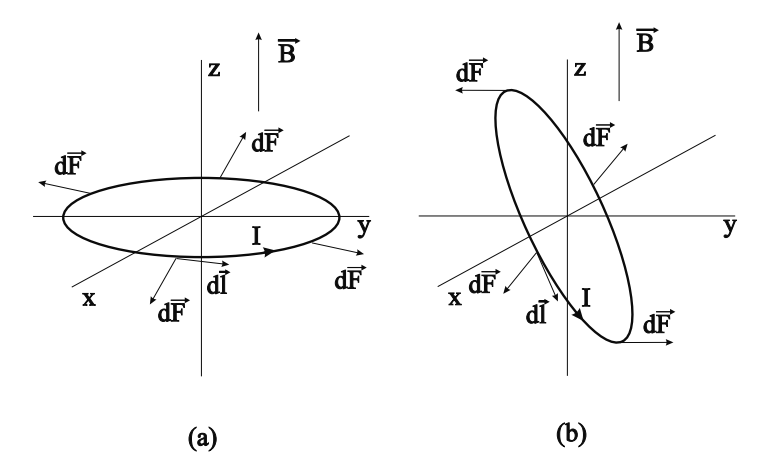
\includegraphics[width=0.6\textwidth,keepaspectratio]{fig21}
%     	\caption{
%        Circular current loop depicted in two different orientations relative to a uniform magnetic
%     field. The forces on representative differential current segments are shown (one \textit{d} is explicitly shown
%     in each case). The first (a) shows the current plane perpendicular to the field where there is no
%     net twist (torque); the second (b) shows the current plane at an arbitrary angle to the field where
%     there is a nonzero torque. 
%         }
%     	\label{fig:fig21}
%     \end{figure}

%     \item In other words, if the current loop is not at rest, then it will try to rotate itself to be at rest. Rotations can also arise from forces applied off-centre even when the sum of all differential forces is zero. Rotations are described by a force called \textbf{torque}. Each differential segment experiences a differential torque: \\
%     \begin{equation}
%         d\vec{N} = \vec{r} \times d\vec{F}
%     \end{equation}

%     \item The total sum of these differential torques is zero for non-rotating objects, and nonzero for rotating ones. This is exemplified in Figure~\ref{fig:fig21} and in Exercises \ref{fig:prbl21} and \ref{fig:prbl22}.

%     \item For any arbitrary current distribution, the net torque has the following formula: \\
%     \begin{equation} \label{eq:eq24}
%         \vec{N} = \vec{\mu} \times \vec{B}
%     \end{equation}
%     where $\vec{\mu}$ is called the magnetic dipole moment or magnetic moment. 
    
%     \item The magnetic moment vector for planar loops is given in
%         terms of the current going through the loop \textit{I}, the area of the
%         loop \textit{A} and the unit vector $\vec{n}$ perpendicular to the
%         current loop plane \\
%     \begin{equation} \label{eq:eq25}
%         \vec{\mu} = I A \hat{n}
%     \end{equation}
%     This can be visualised in Figure~\ref{fig:fig22}.
%     \begin{figure}[H]
%     	\centering
%     	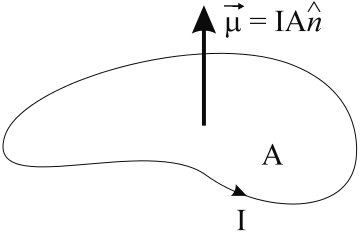
\includegraphics[width=0.4\textwidth,keepaspectratio]{fig22}
%     	\caption{ A loop with current I lying in a plane
%         } 
%     	\label{fig:fig22}
%     \end{figure}
    
    
%     \item An example: For Figure~\ref{fig:fig23a}, 
%         the total torque for planar loops will depend on the current
%         \textit{I} (anticlockwise), the magnetic field strength \textit{B}, the angle
%         \textit{$\theta$} between the plane in which the current loop lies and the
%         magnetic field and the total area of the loop. \\
%     To get to this we begin with: \\
%     $d\vec{N} = \vec{r} \times (Id\vec{l} \times \vec{B}) = Id\vec{l}(\vec{B} \cdot \vec{r}) - I \vec{B} (d\vec{l} \cdot \vec{r})$ \\
%     with $\vec{B}$ and the cylindrical unit vectors looking like:
%     \begin{align}
%         \vec{B} = B(cos \theta \text{ } \hat{z} + sin \theta \text{ } \hat{y}) \\
%         \hat{\rho} = cos \phi \text{ } \hat{x} + sin \phi \text{ } \hat{y} \\
%         \hat{\phi} = - sin \phi \text{ } \hat{x} + cos \phi \text{ } \hat{y}
%     \end{align}
%     Calculating and integrating over we get to:
%     \begin{equation} \label{eq:eq29}
%         \vec{N} = − I \pi R 2 B sin\theta \hat{x}
%     \end{equation}
%     \begin{figure}[H]
%     	\centering
%     	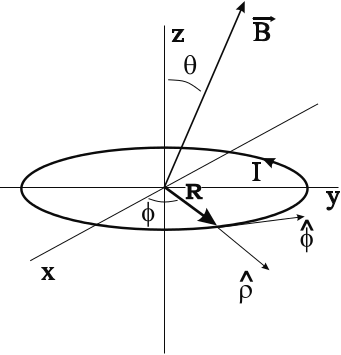
\includegraphics[width=0.4\textwidth,keepaspectratio]{fig23a}
%     	\caption{ A circular loop in x-y plane and the magnetic field lying in the y-z plane
%         } 
%     	\label{fig:fig23a}
%     \end{figure}
    
% \end{itemize}


% \subsubsection{Magnet Toy Model}
% \begin{itemize}

%     \item The picture so far can also be painted from the perspective of a dipole: 
%     2 positive and negative charges at distance $d$ one from another. 
%     In this frame we will also get a net torque of the same form as discussed before:

%     \item In terms of magnetic dipoles (see Figure~\ref{fig:fig23c}), the magnetic moment vector 
%         has the following form: \\
%         \begin{equation}  \label{eq:eq211}
%             \vec{\mu}_m = \hat{n} q_m d
%         \end{equation}
%         where $d$ is the distance between
%         the magnetic charges ($-q_m$ and $+q_m$) \\
%         The force on the magnetic charge due to a magnetic field is:\\
%         \begin{equation}  \label{eq:eq212}
%             \vec{F}_m = q_m \vec{B}
%         \end{equation}
%         Therefore, by choosing the torque reference point to lie on the
%         negative charge, the net torque will be: \\
%         $\vec{N}_m = (\hat{z}d) \times (q_m \vec{B}) $
%     \begin{figure}[H]
%     	\centering
%     	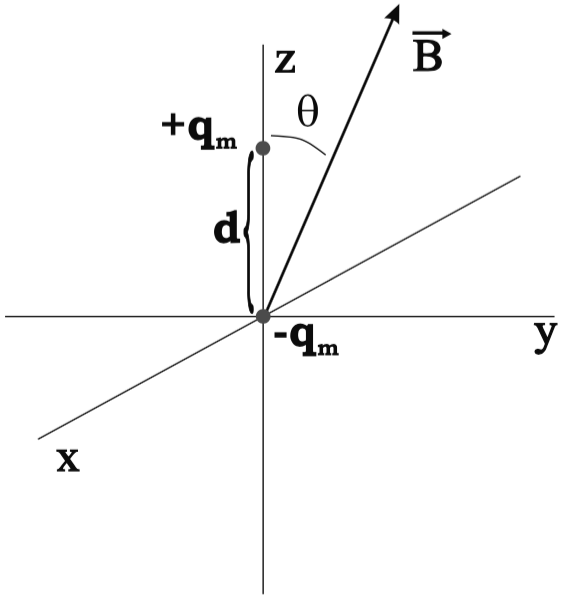
\includegraphics[width=0.4\textwidth,keepaspectratio]{fig23c}
%     	\caption{ A magnetic charge pair along the z axis } 
%     	\label{fig:fig23c}
%     \end{figure}
% \end{itemize}


% %%%%%%%%%%%%%%%%%%
% \clearpage
% %%%%%%%%%%%%%%%%%%%%%%%%%%%%%%%%%%%%%%%%%%
% \subsection{Magnetic Moment with Spin: Equation of Motion}
% \begin{itemize}
%     \item This section introduces angular momentum to the picture painted before.
% \end{itemize}

% %%%
% \subsubsection{Torque and Angular Momentum}
% \begin{itemize}
%     \item The change in the angular momentum of the spin will equal torque.
%     \begin{equation} \label{eq:eq214}
%         \frac{d\vec{J}}{dt} = \vec{N}
%     \end{equation}
    
%     \item This comes from:
%     \begin{equation} \label{eq:eq215}
%         \vec{J} = \sum_i \vec{r}_i \times \vec{p}_i
%     \end{equation}
%     where $d\vec{p} = \vec{F} dt$
    
    
%     \textcolor{gray}{\textbf{Sidenote}: \\
%     $\vec{p}$ is linear momentum \\
%     $\vec{r} \times \vec{p}$ is angular momentum    
%     }
% \end{itemize}

% %%%
% \subsubsection{Angular Momentum of the Proton}
% \begin{itemize}
%     \item 
% \end{itemize}


% %%%
% \subsubsection{Electrons and Other Elements}
% \begin{itemize}
%     \item 
% \end{itemize}

% %%%
% \subsubsection{Equation of Motion}
% \begin{itemize}
%     \item 
% \end{itemize}

% %%%%%%%%%%%%%%%%%%
% \clearpage
% %%%%%%%%%%%%%%%%%%%%%%%%%%%%%%%%%%%%%%%%%%
% \subsection{Precession Solution: Phase}
% \begin{itemize}
%     \item 
% \end{itemize}

% %%%
% \subsubsection{Precession via the Gyroscope Analogy}
% \begin{itemize}
%     \item 
% \end{itemize}

% %%%
% \subsubsection{Geometrical Representation}
% \begin{itemize}
%     \item 
% \end{itemize}

% %%%
% \subsubsection{Cartesian Representation}
% \begin{itemize}
%     \item 
% \end{itemize}

% %%%
% \subsubsection{Matrix Representation}
% \begin{itemize}
%     \item 
% \end{itemize}

% %%%
% \subsubsection{Complex Representation and Phase}
% \begin{itemize}
%     \item 
% \end{itemize}





% \clearpage
% {\huge Old Notes} \\

% In this chapter, and the next, the focus is on the basic element of the first stage, a
% single proton's response to an external field, ignoring the interactions of each proton with
% its surroundings.

% %%%%%%%%%%%%%%%%%%%%%%%%%%%%%%%%%%%%%%%%%%
% \subsection{Torque on a Current Loop in a Magnetic Field}
% When an external field $\vec{B}$ is turned on, a circular loop of current I and area A will feel a differential force on each of its differential segments d$\vec{l}$ given by the basic Lorentz force law:




% The total force on the circular loop, and indeed on any closed loop, due to a uniform
% (constant over space) external magnetic field is zero. 
% Zero total force means zero change in the total momentum $\vec{p}$, from Newton's law:


% Therefore, a current loop initially at rest in a spatially constant magnetic field stays at rest.
% But, it can be rotated by the field. The vector quantity used to describe the rotation of an object is torque:


% The formula for the net torque on any current distribution, which is exact in a 
% constant magnetic field, is given in terms of the \textit{magnetic dipole moment} 
% or simply \textit{magnetic moment} $\mu$:


% The magnetic moment vector for planar loops is given by (and see Figure~\ref{fig:fig22})



% For Figure~\ref{fig:fig23a} the differential torque on $d\vec{l}$ can be written quite generally as:






% \textbf{Takeaway:} A magnetic moment, such as that corresponding to a current loop or a bar magnet, 
% will try to line up along the direction of an external magnetic field.

% %%%%%%%%%%%%%%%%%%%%%%%%%%%%%%%%%%%%%%%%%%
% \subsection{Magnetic Moment with Spin: Equation of Motion}
% Nonzero total torque on a system implies that the system’s total angular momentum J must
% change according to:
% \begin{equation} \label{eq:eq214}
%     \frac{d\vec{J}}{dt} = \vec{N}
% \end{equation}

% The direct relationship between the magnetic moment and
% the spin angular momentum vector is found from experiment:
% \begin{equation} \label{eq:eq216}
%     \vec{\mu} = \gamma \vec{J}
% \end{equation}

% Using Eq~\ref{eq:eq216} and Eq~\ref{eq:eq24} in Eq~\ref{eq:eq214}, we get 
% the fundamental equation of motion (a simple version of the Bloch equation):
% \begin{equation} \label{eq:eq224}
%     \frac{d\vec{\mu}}{dt} = \gamma \vec{\mu} \times \vec{B}
% \end{equation}

% %%%%%%%%%%%%%%%%%%%%%%%%%%%%%%%%%%%%%%%%%%
% \subsection{Geometrical Representation}
% \begin{multicols}{2}
% \begin{align*}
%     R = \abs{\mu} \cdot sin\theta \\
%     d\vec{\mu} = R \cdot \abs{d\phi} \\
%     d\vec{\mu} = \abs{\vec{\mu}} \cdot sin\theta \cdot \abs{d\phi}
% \end{align*}

% \vfill
% \columnbreak

% \begin{figure}[H]
% 	\centering
% 	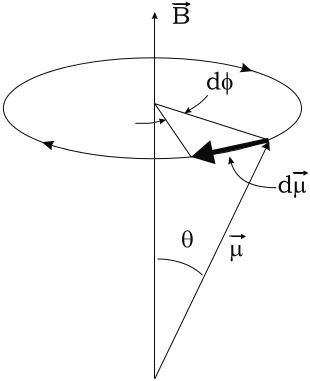
\includegraphics[width=0.3\textwidth,keepaspectratio]{fig25}
% 	\caption{ Clockwise precession of a proton's spin about a magnetic field.
%     } 
% 	\label{fig:fig25}
% \end{figure}

% \end{multicols}

% %\clearpage

% \begin{equation}\label{eq:eq225}
%     \abs{d\vec{\mu}} = \mu\, sin\theta\, \abs{d\phi}
% \end{equation}
% From Eq~\ref{eq:eq224}:
% \begin{equation}\label{eq:eq226}
%     \abs{d\vec{\mu}} = \gamma \abs{\vec{\mu} \times \vec{B}} dt = \gamma\, \mu\, B\, sin \theta\, dt
% \end{equation}
% From Eq~\ref{eq:eq225} and ~\ref{eq:eq226} we have: $\abs{d\phi} = \gamma\, B\,dt$.\\
% Because $\omega = \abs{\frac{d\phi}{dt}}$, we get the famous Larmor precession formula:
% \begin{equation}\label{eq:eq227}
%     \omega = \gamma\, B
% \end{equation}
% Also, because we have a clockwise rotation in the figure:
% \begin{equation}\label{eq:eq228}
%     \frac{d\phi}{dt} = - \omega
% \end{equation}
% If the field is along the z-axis and constant in time, $\vec{B} = B_0 \hat{z}$,
% the solution for Eq~\ref{eq:eq228} is:
% \begin{equation}\label{eq:eq230}
%     \phi = - \omega_0 t + \phi_0
% \end{equation}

% %%%%%%%%%%%%%%%%%%%%%%%%%%%%%%%%%%%%%%%%%%
% \subsection{Cartesian Representation}
% \begin{multicols}{2}
% \begin{align*}
%     \vec{\mu_x}(t) = \vec{\mu}(t) \cdot cos(\phi_0 - \xi) \\
%     \vec{\mu_x}(t) = \vec{\mu}(t) \cdot (cos \phi_0 \cdot cos \xi + sin \phi_0 \cdot sin \xi ) \\
%     \vec{\mu_x}(t) = \vec{\mu}(t) \cdot cos \phi_0 \cdot cos \xi \\
%     + \vec{\mu}(t) \cdot sin \phi_0 \cdot sin \xi  \\
%     \vec{\mu_x}(t) = \vec{\mu}(t) \cdot \frac{\vec{\mu_x}(0)}{\vec{\mu}(0)} \cdot cos \xi \\
%     + \vec{\mu}(t) \cdot  \frac{\vec{\mu_y}(0)}{\vec{\mu}(0)} \cdot sin \xi  \\
%     \vec{\mu_x}(t) = \vec{\mu_x}(0) \cdot cos \xi + \vec{\mu_y}(0) \cdot sin \xi \\
% \end{align*}

% \vfill
% \columnbreak

% \begin{figure}[H]
% 	\centering
% 	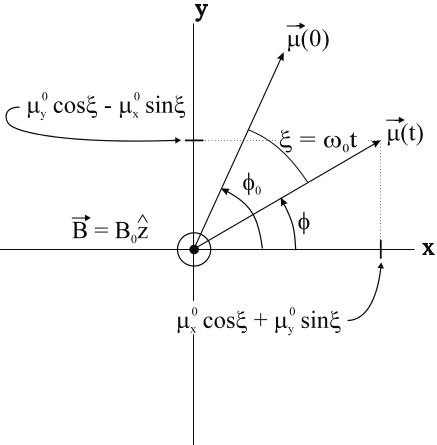
\includegraphics[width=0.4\textwidth,keepaspectratio]{fig26a}
% 	\caption{ } 
% 	\label{fig:fig26a}
% \end{figure}

% \end{multicols}

% For $\vec{B} = B_0 \hat{z}$ we have:
% \begin{equation}\label{eq:eq232}
%     \vec{\mu}(t) = \vec{\mu_x}(t)\hat{x} + \vec{\mu_y}(t)\hat{y} +  \vec{\mu_z}(t)\hat{z}
% \end{equation}
% with:
% \begin{align}\label{eq:eq233}
%     {\mu_x}(t) = {\mu_x}(0) \cdot cos \omega_0 t + {\mu_y}(0) \cdot sin \omega_0 t \\
%     {\mu_y}(t) = {\mu_y}(0) \cdot cos \omega_0 t - {\mu_x}(0) \cdot sin \omega_0 t \\
%     {\mu_z}(t) = {\mu_z}(0)
% \end{align}

% %%%%%%%%%%%%%%%%%%%%%%%%%%%%%%%%%%%%%%%%%%
% \subsection{Matrix Representation}
% \begin{equation}\label{eq:eq236}
%     \vec{\mu}(t) = R_z(\omega_0t) \vec{\mu}(0)
% \end{equation}
% with:
% \begin{equation}
% R_z(\theta)=
% \begin{pmatrix}
% cos\theta & sin\theta & 0 \\
% -sin\theta & cos\theta & 0 \\
% 0 & 0 & 1
% \end{pmatrix}
% \end{equation}

% %%%%%%%%%%%%%%%%%%%%%%%%%%%%%%%%%%%%%%%%%%
% \subsection{Complex Representation and Phase}
% The two degrees of freedom, ${\mu_x}$ and ${\mu_y}$, can be given in terms of the real and
% imaginary parts of:
% \begin{equation}
%     {\mu_{+}}(t) = {\mu_x}(t) + i {\mu_y}(t)
% \end{equation}
% with:
% \begin{equation}
%     {\mu_{+}}(t) = {\mu_{+}}(0) e^{-i\omega_0t}
% \end{equation}

% In general, the complex number ${\mu_{+}}(t)$ can be written in terms of its magnitude and phase:
% \begin{equation}
%     {\mu_{+}}(t) = \abs{{\mu_{+}}(t)} e^{i\phi (t)}
% \end{equation}
% So, the complex representation can be rewritten as:
% \begin{equation}
%     {\mu_{+}}(t) = \abs{{\mu_{+}}(0)} e^{i\phi_0 (t)}
% \end{equation}
% where the phase is:
% \begin{equation}
%     \phi_0(t) = -\omega_0 t + \phi_0(0)
% \end{equation}






\clearpage
%%%%%%%%%%%%%%%%%%%%%%%%%%%%%%
%% EXERCISES
\newpage
\subsection{Exercises}

%%%%%%%%%%%%%%%%%%%%%%%%%%%%%%%
\Large{Problem 2.1}
\label{ex:ex21}

\begin{figure}[H]
        \centering
        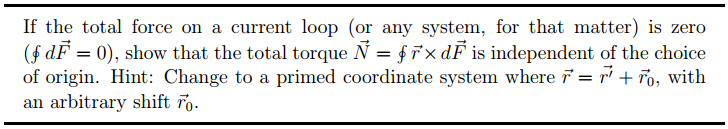
\includegraphics[width=0.8\textwidth,keepaspectratio]{prbl21}
        \label{fig:prbl21}
\end{figure}

\textit{Remember:}
\begin{itemize}
	\item Zero total force means zero change in the total momentum (conservation 
of momentum).
	\item Rotations can arise (about the centre of mass) from forces applied off centre, even 
	when the vector sum of all forces cancels out.
	\item The total torque is independent of the choice of origin.
\end{itemize}

\begin{align*}
\oint d\vec{F}  = 0 \\
\vec{N}  = \oint \vec{r} \times d\vec{F} \\
\vec{r}  = \vec{r'} + \vec{r_{0}}
\end{align*}

%\begin{proof}
\textit{Proof.}
\begin{align*}
\vec{N'} & = \oint (\vec{r} - \vec{r_{0}}) \times d \vec{F} \\ 
\vec{N'} & = \oint \vec{r} \times d\vec{F} - \oint \vec{r_0} \times d\vec{F} \\
\end{align*}
\[
\begin{rcases*}
\vec{N'} = \oint \vec{r} \times d\vec{F} - \vec{r_0} \times \oint d\vec{F} \\
\text{We know that: } \oint d\vec{F} = 0 \\
\end{rcases*} \vec{N'} = \oint \vec{r} \times d\vec{F} = \vec{N}
\]
%\end{proof}

\clearpage

%%%%%%%%%%%%%%%%%%%%%%%%%%%%%%%
\Large{Problem 2.2}
\label{ex:ex22}

\begin{figure}[H]
        \centering
        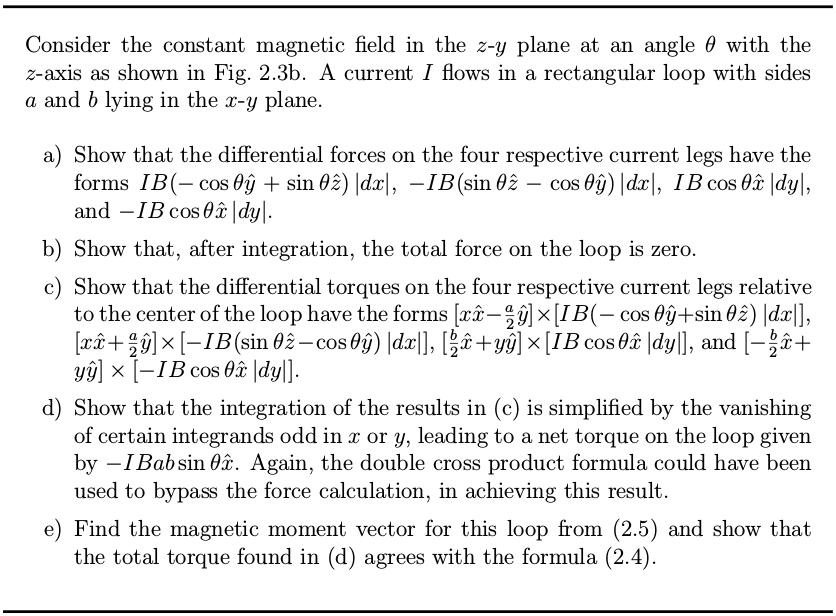
\includegraphics[width=0.8\textwidth,keepaspectratio]{prbl22}
        \label{fig:prbl22}
\end{figure}

\begin{figure}[H]
        \centering
        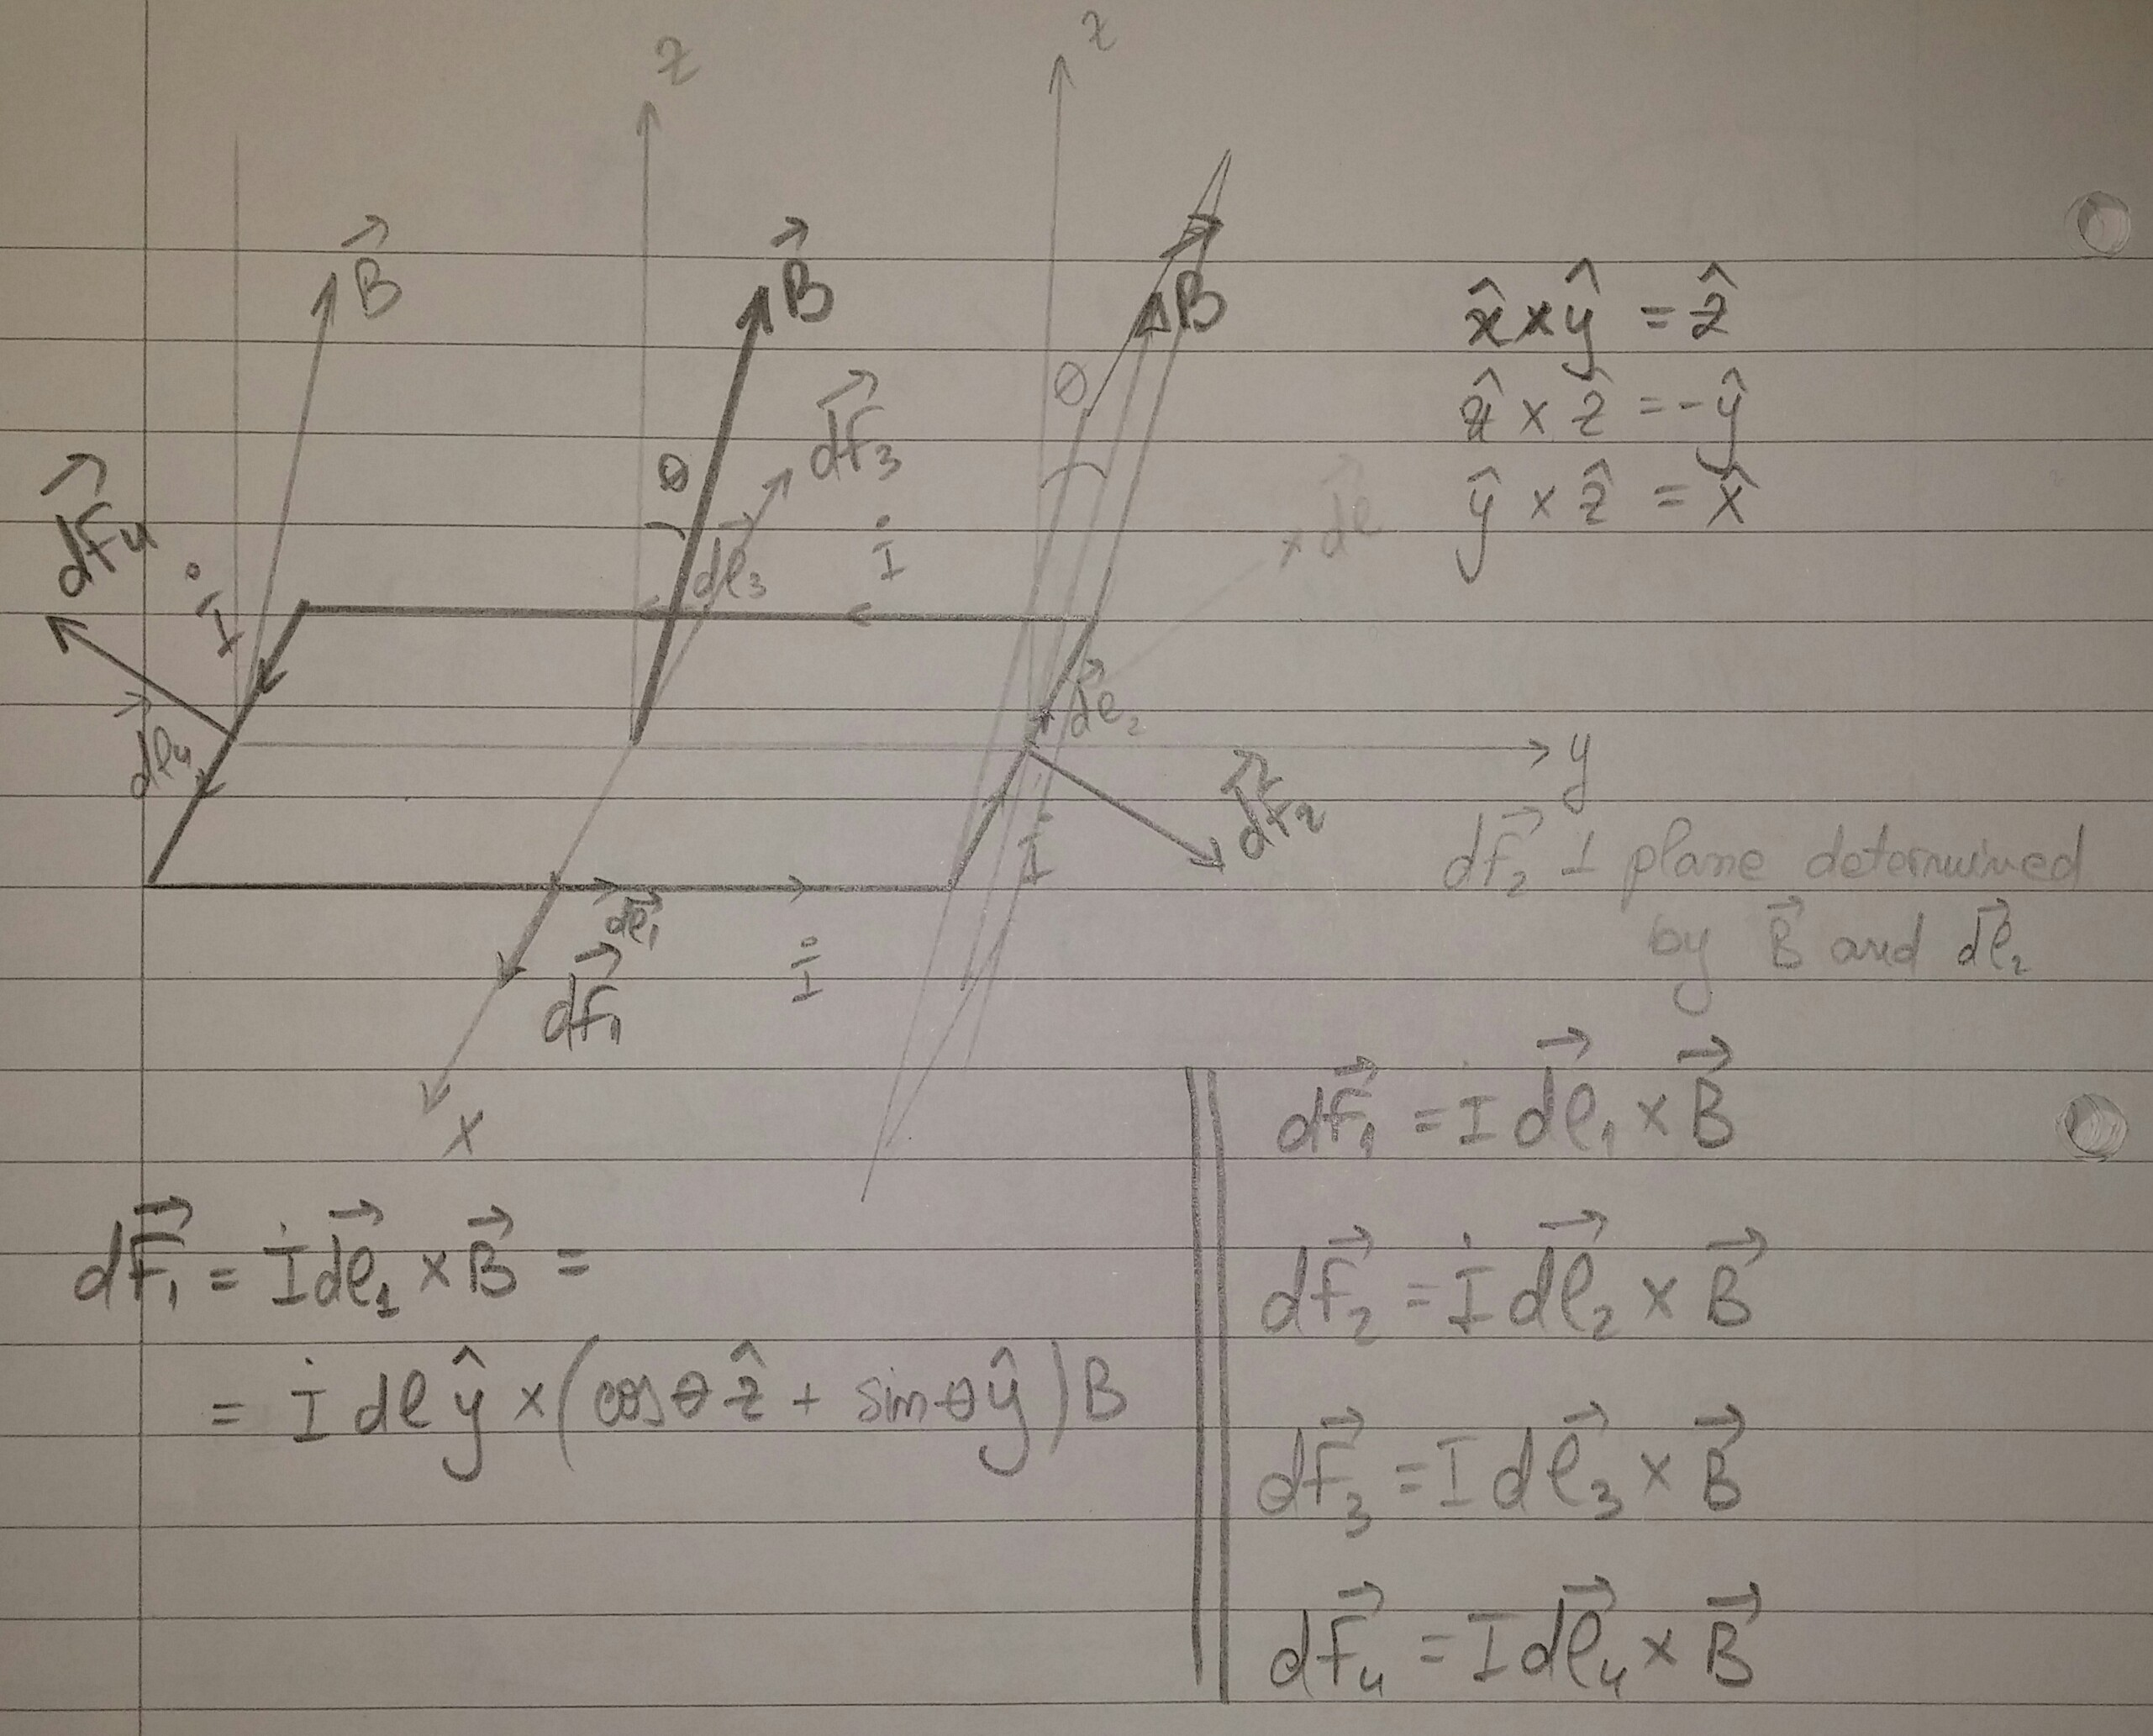
\includegraphics[width=.9\textwidth,keepaspectratio]{problem22}
        \label{fig:problem22}
\end{figure}

\textit{Remember:}
\begin{itemize}
	\item A rectangular loop behaves in a similar fashion as a 
	circular one.
	\item The total force on the loop is zero.
	\item The total torque depends on the dimensions of the loop.
\end{itemize}

\begin{wrapfigure}{r}{0.4\textwidth}
  \begin{center}
    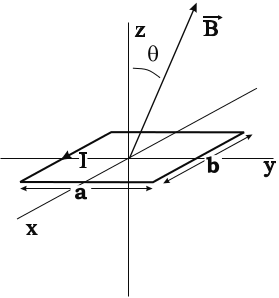
\includegraphics[width=0.38\textwidth]{fig23b}
  \end{center}
  \caption{current loops lying in the x-y plane and a magnetic charge pair along the z-axis}
\end{wrapfigure}

\textit{We know:}\\
\begin{flalign*}
    \hat{x} \times \hat{y} &= \hat{z} \\
    \hat{x} \times \hat{z} &= - \hat{y} \\
    \hat{y} \times \hat{z} &= - \hat{x} \\ \\
    \vec{B} &= \vec{B_y} + \vec{B_z} \\
    \vec{B} &= (cos \theta \hat{z} + sin \theta \hat{y})B
\end{flalign*}

\textit{a) Proof.}\\ \\
A current I flowing through a loop placed in an external magnetic field B will experience a differential force on the loop determined by:
\begin{equation} 
    d\vec{F} = I d\vec{l} \times \vec{B} \\ \\ %\Longrightarrow \\ \\
\end{equation}

As this loop has a rectangular shape, each side of the loop will experience a differential force determined by its respective differential segments. These differential segments $d\vec{l}$ will 

We get:
\begin{flalign*}
d\vec{F_{1}} &= I \vec{dl_1} \times \vec{B} \\
             &= I \abs{dl} \hat{y} \times (cos \theta \hat{z} + sin \theta \hat{y}) B \\
             &= I B cos\theta \hat{x} \abs{dl} \\
d\vec{F_{2}} &= I \vec{dl_2} \times \vec{B} \\
             &= - I \abs{dl} \hat{x} \times (cos \theta \hat{z} + sin \theta \hat{y}) B \\
             &= I B cos\theta \hat{y} \abs{dl} - I B sin\theta \hat{z} \abs{dl} \\
d\vec{F_{3}} &= I \vec{dl_3} \times \vec{B} \\
             &= - I \abs{dl} \hat{y} \times (cos \theta \hat{z} + sin \theta \hat{y}) B \\
             &= - I B cos\theta \hat{x} \abs{dl} \\
d\vec{F_{4}} &= I \vec{dl_4} \times \vec{B} \\
             &= I \abs{dl} \hat{x} \times (cos \theta \hat{z} + sin \theta \hat{y}) B \\
             &= - I B cos\theta \hat{y} \abs{dl} + I B sin\theta \hat{z} \abs{dl}
\end{flalign*}


\textit{b) Proof.}
\begin{align*}
\vec{F} &= d\vec{F_1} + d\vec{F_2} + d\vec{F_3} + d\vec{F_4} \\
\vec{F} &= I B cos\theta \hat{x} \abs{dl} 
         + I B cos\theta \hat{y} \abs{dl} 
         - I B sin\theta \hat{z} \abs{dl} \\
        &- I B cos\theta \hat{x} \abs{dl}
         - I B cos\theta \hat{y} \abs{dl} 
         + I B sin\theta \hat{z} \abs{dl}\\
& = 0
\end{align*}

\textit{c) Proof.}
\begin{align*}
    d\vec{N_i} &= \vec{r_i} \times d\vec{F_i} \\ \\
    \vec{r_1} &= \frac{b}{2} \hat{x} + y \hat{y} \\
    \vec{r_2} &= x \hat{x} + \frac{a}{2} \hat{y} \\
    \vec{r_3} &= - \frac{b}{2} \hat{x} + y \hat{y} \\
    \vec{r_2} &= x \hat{x} - \frac{a}{2} \hat{y} \\ \\
    d\vec{N_1} &= (\frac{b}{2} \hat{x} + y \hat{y}) \times (I B cos\theta \hat{x} \abs{dl}) \\ 
               &= -IBcos\theta y \abs{dl} \hat{z} \\
    d\vec{N_2} &= (x \hat{x} + \frac{a}{2} \hat{y}) \times (I B cos\theta \hat{y} \abs{dl} - I B sin\theta \hat{z} \abs{dl}) \\ 
               &= IBcos\theta x \abs{dl} \hat{z}  - IBsin\theta\abs{dl} (-x\hat{y} + \frac{a}{2}\hat{x}) \\
    d\vec{N_3} &= (- \frac{b}{2} \hat{x} + y \hat{y}) \times (- I B cos\theta \hat{x} \abs{dl}) \\ 
			   &= IBcos\theta y \abs{dl} \hat{z} \\
    d\vec{N_4} &= (x \hat{x} - \frac{a}{2} \hat{y}) \times (- I B cos\theta \hat{y} \abs{dl} + I B sin\theta \hat{z} \abs{dl}) \\ 
			   &= -IBcos\theta x \abs{dl} \hat{z}  + IBsin\theta\abs{dl} (-x\hat{y} - \frac{a}{2}\hat{x}) \\
\end{align*}

\textit{d) Proof.}
\begin{align*}
\vec{N} &= \int_{-a/2}^{a/2} d\vec{N_1} + \int_{-b/2}^{b/2} d\vec{N_2} 
         + \int_{-a/2}^{a/2}d\vec{N_3} + \int_{-b/2}^{b/2}d\vec{N_4} \\
        &= \int_{-a/2}^{a/2} d\vec{N_1} + d\vec{N_3} + \int_{-b/2}^{b/2} d\vec{N_2} + d\vec{N_4} \\
        &= 0 + \int_{-b/2}^{b/2} IBsin\theta\abs{dl} (\cancel{-x\hat{y}} - \frac{a}{2}\hat{x} \cancel{+ x\hat{y}} - \frac{a}{2}\hat{x}) dx \\
        &= -IB ab \ sin\theta \hat{x}
\end{align*}

\textit{e) Proof.}
\begin{align*}
\vec{N} &= \vec{\mu} \times \vec{B} \\
        &= I A \ \hat{n} \times \vec{B} \\
        &= I ab \ \hat{n} \times \vec{B} \\
        &= - I B ab \ sin\theta \hat{x}\\
\end{align*}


\clearpage
%%%%%%%%%%%%%%%%%%%%%%%%%%%%%%%
\Large{Problem 2.3}

\begin{figure}[H]
        \centering
        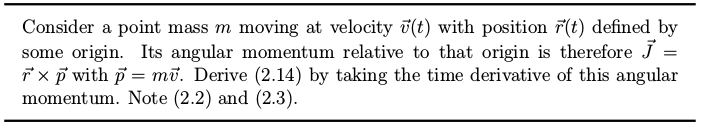
\includegraphics[width=0.8\textwidth,keepaspectratio]{prbl23}
        \label{fig:prbl23}
\end{figure}

\textit{Remember:}
\begin{itemize}
	\item A magnetic moment will try to line up along the direction of 
	an external magnetic field.
	\item If the system has nonzero total torque $\vec{N}$, then the 
	system's total angular momentum $\vec{J}$ changes according to 
	$\frac{d\vec{J}}{dt} = \vec{N}$.
\end{itemize}

(2.14) $\frac{d\vec{J}}{dt} = \vec{N}$ \\ \\
(2.2) $\vec{F} = \frac{d\vec{p}}{dt}$ \\ \\
(2.3) $d\vec{N} = \vec{r} \times d\vec{F}$.\\  \\
\textit{Proof.}
\begin{align*}
    \vec{J} & = \vec{r} \times \vec{p} \\
    \frac{d\vec{J}}{dt} & = \frac{d\vec{r}}{dt} \times \vec{p} + \vec{r} \times \frac{d\vec{p}}{dt} \\
    & = \vec{v} \times \vec{p} + \vec{r} \times \vec{F} \\
    & = \vec{v} \times (m \cdot \vec{v} ) + \vec{r} \times \vec{F} \\
    & = \mathbf{0} + \vec{N} = \vec{N}
\end{align*} 

\clearpage
%%%%%%%%%%%%%%%%%%%%%%%%%%%%%%%
\Large{Problem 2.4}

\begin{figure}[H]
        \centering
        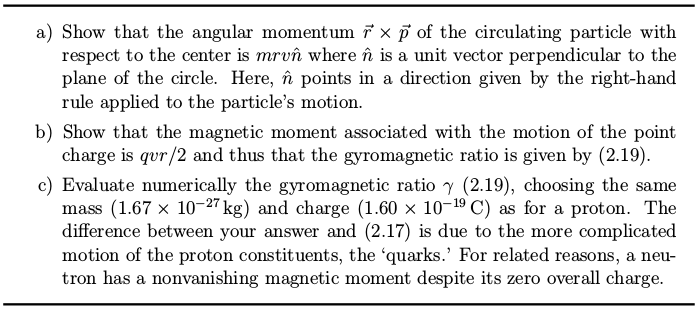
\includegraphics[width=0.8\textwidth,keepaspectratio]{prbl24}
        \label{fig:prbl24}
\end{figure}

\textit{Remember:}
\begin{itemize}
	\item The relationship between angular momentum and magnetic 
	moment is given by $\vec{\mu} = \gamma \vec{J}$
	\item In classic terms, the angular momentum depends on the mass 
	and velocity of the circulating particle.
	\item The current $I = \frac{q}{t}$ is the flux of charge in time.
	\item There are differences due to mass between different types of 
	of circulating particles.
\end{itemize}

\textit{a) Proof.}
\begin{align*}
    \vec{r} \times \vec{p} & = \vec{r} \times (m \cdot \vec{v}) \\
    & = m r v \ sin\theta \hat{n}\\
    \text{ with } \theta & = 90^0 \Rightarrow \\
    \vec{r} \times \vec{p} & = m r v \hat{n}
\end{align*}

\textit{b) Proof.}
\begin{align*}
	\vec{\mu} &= \gamma \vec{J} \\
	          &= \gamma \vec{r} \times \vec{p} \\
	          &= \gamma m r v \hat{n}\ (1) \\
	\vec{\mu} &= I A \hat{n} \\
	          &= \frac{q}{T} \ \pi r^2 \hat{n} \\
	          &= \frac{q \, v}{2 \cancel{\pi} \cancel{r}} \ \cancel{\pi} 
	          r^{\cancel{2}} \hat{n}  \\
	          &= \frac{qvr}{2} \, \hat{n} \, (2)
\end{align*}
\begin{align*}
\text{From (1) and (2)} \Rightarrow \frac{q\cancel{vr}}{2} \, \hat{n} 
\,  &= \gamma m \cancel{vr} \hat{n} \\
			\hat{n} \, (\frac{q}{2} - \gamma m) &= 0 \\
			\frac{q}{2} - \gamma m &= 0 \\
			\gamma m &= \frac{q}{2} \\
			\gamma &= \frac{q}{2m}
\end{align*}

\clearpage
%%%%%%%%%%%%%%%%%%%%%%%%%%%%%%%
\Large{Problem 2.5}

\begin{figure}[H]
        \centering
        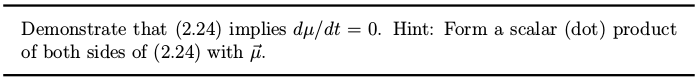
\includegraphics[width=0.8\textwidth,keepaspectratio]{prbl25}
        \label{fig:prbl25}
\end{figure}

\textit{Remember:}
\begin{itemize}
	\item The magnitude of $\vec{\mu}$ does not change in time.
\end{itemize}


\textit{Proof.} \\
Dot product on the right hand side: \\
\begin{flalign*}
    \frac{d\vec{\mu}}{dt} & = \gamma \vec{\mu} \times \vec{B} \\
    \frac{d\vec{\mu}}{dt} \cdot \vec{\mu} & = \gamma (\vec{\mu} \times \vec{B}) \cdot \vec{\mu} \\
    \frac{d\vec{\mu}}{dt} \cdot \vec{\mu} & = (\gamma\, \mu \, B \, 
    sin\theta \, \hat{n}) \cdot \vec{\mu} \\
    \text{Obs: } \hat{n} \text{ is orthogonal to } \vec{\mu} & \Rightarrow cos(\angle( \hat{n}, \vec{\mu})) = 0 \Rightarrow \\
    \frac{d\vec{\mu}}{dt} \cdot \vec{\mu} & = 0 \, (1) \\
\end{flalign*}
Dot product on the left hand side: \\
\begin{flalign*}
    \vec{\mu} \cdot \frac{d\vec{\mu}}{dt} & = \gamma (\vec{\mu} \times \vec{B}) \cdot \vec{\mu} \\
    \vec{\mu} \cdot \frac{d\vec{\mu}}{dt} & = \vec{\mu} \cdot (\gamma\, 
    \mu \, B \, sin\theta \, \hat{n})\\
    \text{Obs: } \hat{n} \text{ is orthogonal to } \vec{\mu} & \Rightarrow cos(\angle( \hat{n}, \vec{\mu})) = 0 \Rightarrow \\
    \vec{\mu} \cdot \frac{d\vec{\mu}}{dt} &= 0 \, (2)\\
\end{flalign*}

From (1) + (2) we get: \\
\begin{flalign*}
	\frac{d\vec{\mu}}{dt} \cdot \vec{\mu} + \vec{\mu} \cdot 
	\frac{d\vec{\mu}}{dt} &= 0 \\
	\frac{d(\vec{\mu} \cdot \vec{\mu})}{dt} &= 0 \\
	\frac{d\mu^2}{dt} &= 0 \\
	\frac{d \mu}{dt} \, \mu + \mu \, \frac{d \mu}{dt} &= 0 \\
	2 \, \mu \, \frac{d \mu}{dt} &= 0 \\
	\frac{d \mu}{dt} &= 0
\end{flalign*}

\clearpage
%%%%%%%%%%%%%%%%%%%%%%%%%%%%%%%
\Large{Problem 2.6}

\begin{figure}[H]
        \centering
        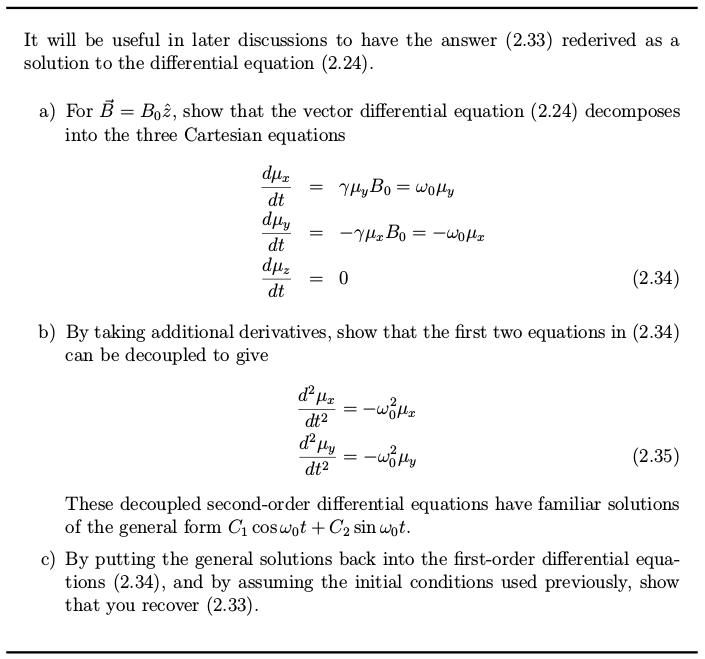
\includegraphics[width=0.8\textwidth,keepaspectratio]{prbl26}
        \label{fig:prbl26}
\end{figure}

\textit{Remember:}
\begin{itemize}
	\item The magnitude of the z-component of the magnetic moment does 
	not change in time, while the xy-components rotate about the z 
	axis.
\end{itemize}

(2.33)
\begin{align*}\label{eq:eq233}
    \vec{\mu_x}(t) & = \vec{\mu_x}(0) \cdot cos \omega_0 t + \vec{\mu_y}(0)   \cdot sin \omega_0 t \\
    \vec{\mu_y}(t) & = \vec{\mu_y}(0) \cdot cos \omega_0 t - \vec{\mu_x}(0)   \cdot sin \omega_0 t \\
    \vec{\mu_z}(t) & = \vec{\mu_z}(0)
\end{align*}

(2.24)
\begin{equation*} 
    \frac{d\vec{\mu}}{dt} = \gamma \vec{\mu} \times      \vec{B}
\end{equation*}

\textit{a) Proof.}
\begin{flalign*}
   \frac{d}{dt} (\vec{\mu_x} + \vec{\mu_y} + \vec{\mu_z} ) & = \gamma (\vec{\mu_x} + \vec{\mu_y} + \vec{\mu_z}) \times (\vec{B_x} + \vec{B_y} + \vec{B_z}) \\
    & = \gamma\, B_0\, (\mu_x \hat{x} + \mu_y \hat{y} + \mu_z\hat{z}) \times \hat{z}\\
    & = \gamma\, B_0\, ( -\mu_x \hat{y} + \mu_y \hat{x}  ) \\
    \frac{d\mu_x}{dt} & = \gamma \mu_y B_0 = \omega_0\,\mu_y \\
    \frac{d\mu_y}{dt} & = - \gamma \mu_x B_0 = - \omega_0\,\mu_x \\
    \frac{d\mu_z}{dt} & = 0
\end{flalign*}

\textit{b) Proof.}
\begin{flalign*}
	\frac{d^2 \mu_x}{dt^2} & = \frac{d}{dt} (\frac{d \mu_x}{dt}) = 
	\omega_0 \frac{d \mu_y}{dt} = -\omega_0^2 \mu_x \\
	\frac{d^2 \mu_y}{dt^2} & = \frac{d}{dt} (\frac{d \mu_y}{dt}) = 
	- \omega_0 \frac{d \mu_x}{dt} = -\omega_0^2 \mu_y \\
\end{flalign*}
%\begin{flalign*}
%   f(t)   &= C_1 \, cos\omega_0 t \, + \, C_2 \, sin \omega_0 t \\
%   f'(t)  &= - C_1 \omega_0 \, sin\omega_0 t + C_2 \omega_0 \, cos \omega_0 t \\
%   f''(t) &= - C_1 \omega_0^2 \, cos\omega_0 t - C_2 \omega_0^2 \, sin \omega_0 t \\
%          & \Rightarrow \\
%   f''(t) &= - \omega_0^2 \, (C_1 \, cos\omega_0 t \, + \, C_2 \, sin \omega_0 t) \\
%   f''(t) &= - \omega_0^2 \, f(t)  \\
%          & \Rightarrow \\
%   \frac{d^2 \mu_x}{dt^2} & = -\omega_0^2 \mu_x \\
%   \frac{d^2 \mu_y}{dt^2} & = -\omega_0^2 \mu_y 
%\end{flalign*}

\textit{c) Proof.}
\begin{flalign*}
   f(t)   &= C_1 \, cos\omega_0 t \, + \, C_2 \, sin \omega_0 t \\
   f(0)   &= C_1 & \Rightarrow C_1 = f(0) \\
   f'(t)  &= - C_1 \omega_0 \, sin\omega_0 t + C_2 \omega_0 \, cos \omega_0 t \\
   f'(0)  &= C_2 \omega_0 & \Rightarrow C_2 = \frac{f'(0)}{\omega_0} \\ \\
\end{flalign*}
\begin{flalign*}
   \mu_x(t) &= C_{1x} \, cos\omega_0 t + C_{2x} sin \omega_0 t \\
   C_{1x} &= \mu_x(0) \\
   C_{2x} &= \frac{d\mu_x(0)}{dt} \frac{1}{\omega_0} = \mu_y(0) \\
          & \Rightarrow \\
   \mu_x(t) &= \mu_x(0) \, cos\omega_0 t + \mu_y(0) sin \omega_0 t \\ \\
\end{flalign*}
\begin{flalign*}
   \mu_y(t) &= C_{1y} \, cos\omega_0 t + C_{2y} sin \omega_0 t \\
   C_{1y} &= \mu_y(0) \\
   C_{2y} &= \frac{d\mu_y(0)}{dt} \frac{1}{\omega_0} = - \mu_x(0) \\
          & \Rightarrow \\
   \mu_y(t) &= \mu_y(0) \, cos\omega_0 t - \mu_x(0) sin \omega_0 t \\ \\
   \mu_z(t) &= \mu_z(0)
\end{flalign*}


\clearpage
%%%%%%%%%%%%%%%%%%%%%%%%%%%%%%%
\Large{Problem 2.7}

\begin{figure}[H]
        \centering
        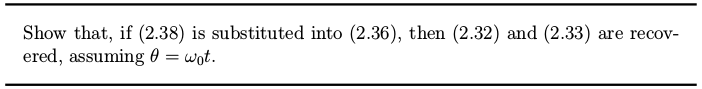
\includegraphics[width=0.8\textwidth,keepaspectratio]{prbl27}
        \label{fig:prbl27}
\end{figure}

\textit{Remember:}
\begin{itemize}
	\item The precession motion of a particle placed in a static 
	magnetic field can be described using a matrix representation.
\end{itemize}

\textit{Proof.}
\begin{flalign*}
\vec{\mu}(t) & = 
\begin{pmatrix}
cos\theta & sin\theta & 0 \\
-sin\theta & cos\theta & 0 \\
0 & 0 & 1
\end{pmatrix}
\cdot \vec{\mu}(0)\\
\begin{pmatrix}
\mu_x(t)\\
\mu_y(t)\\
\mu_z(t)
\end{pmatrix}
& =
\begin{pmatrix}
cos\theta & sin\theta & 0 \\
-sin\theta & cos\theta & 0 \\
0 & 0 & 1
\end{pmatrix}
\cdot
\begin{pmatrix}
\mu_x(0)\\
\mu_y(0)\\
\mu_z(0)
\end{pmatrix}
\Rightarrow \\
    {\mu_x}(t) &= {\mu_x}(0) \cdot cos \omega_0   t + {\mu_y}(0) \cdot sin \omega_0 t \\
    {\mu_y}(t) &= {\mu_y}(0) \cdot cos \omega_0   t - {\mu_x}(0) \cdot sin \omega_0 t \\
    {\mu_z}(t) &= {\mu_z}(0)
\end{flalign*}


\clearpage
%%%%%%%%%%%%%%%%%%%%%%%%%%%%%%%
\Large{Problem 2.8}

\begin{figure}[H]
        \centering
        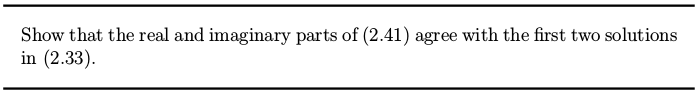
\includegraphics[width=0.8\textwidth,keepaspectratio]{prbl28}
        \label{fig:prbl28}
\end{figure}

\textit{Remember:}
\begin{itemize}
	\item The 2 degrees of freedom, $\mu_x$ and $\mu_y$ can be given 
	in terms of real and imaginary part of $\mu_+$.
	\item Phase directly relates to position and is of utmost 
	importance in the description of spin motion.
\end{itemize}

\textit{Proof.}
\begin{flalign*}
    {\mu_{+}}(t) & = {\mu_{+}}(0) e^{-i\omega_0t}\\
    & = (\mu_{x}(0) + i\, \mu_{y}(0)) \, e^{-i\omega_0t} \\
    & = (\mu_{x}(0) + i\, \mu_{y}(0)) \, (cos\omega_0 t \, - \, i \, sin\omega_0t) \\
    & = \mu_{x}(0) \, cos\omega_0 t - i\, \mu_{x}(0) \, sin\omega_0t + i\, \mu_{y}(0) \, cos\omega_0 t + \mu_{y}(0) sin\omega_0t \\
    & = \mu_x(t) + i \, \mu_y(t)
\end{flalign*}

\clearpage
%%%%%%%%%%%%%%%%%%%%%%%%%%%%%%%
%\Large{Whiteboard Problems}
%
%\begin{figure}[H]
%    \centering
%    \includegraphics[width=0.8\textwidth,keepaspectratio]{Ch2Gary1}
%    \label{fig:Ch2Gary1}
%\end{figure}
%
%\begin{figure}[H]
%    \centering
%    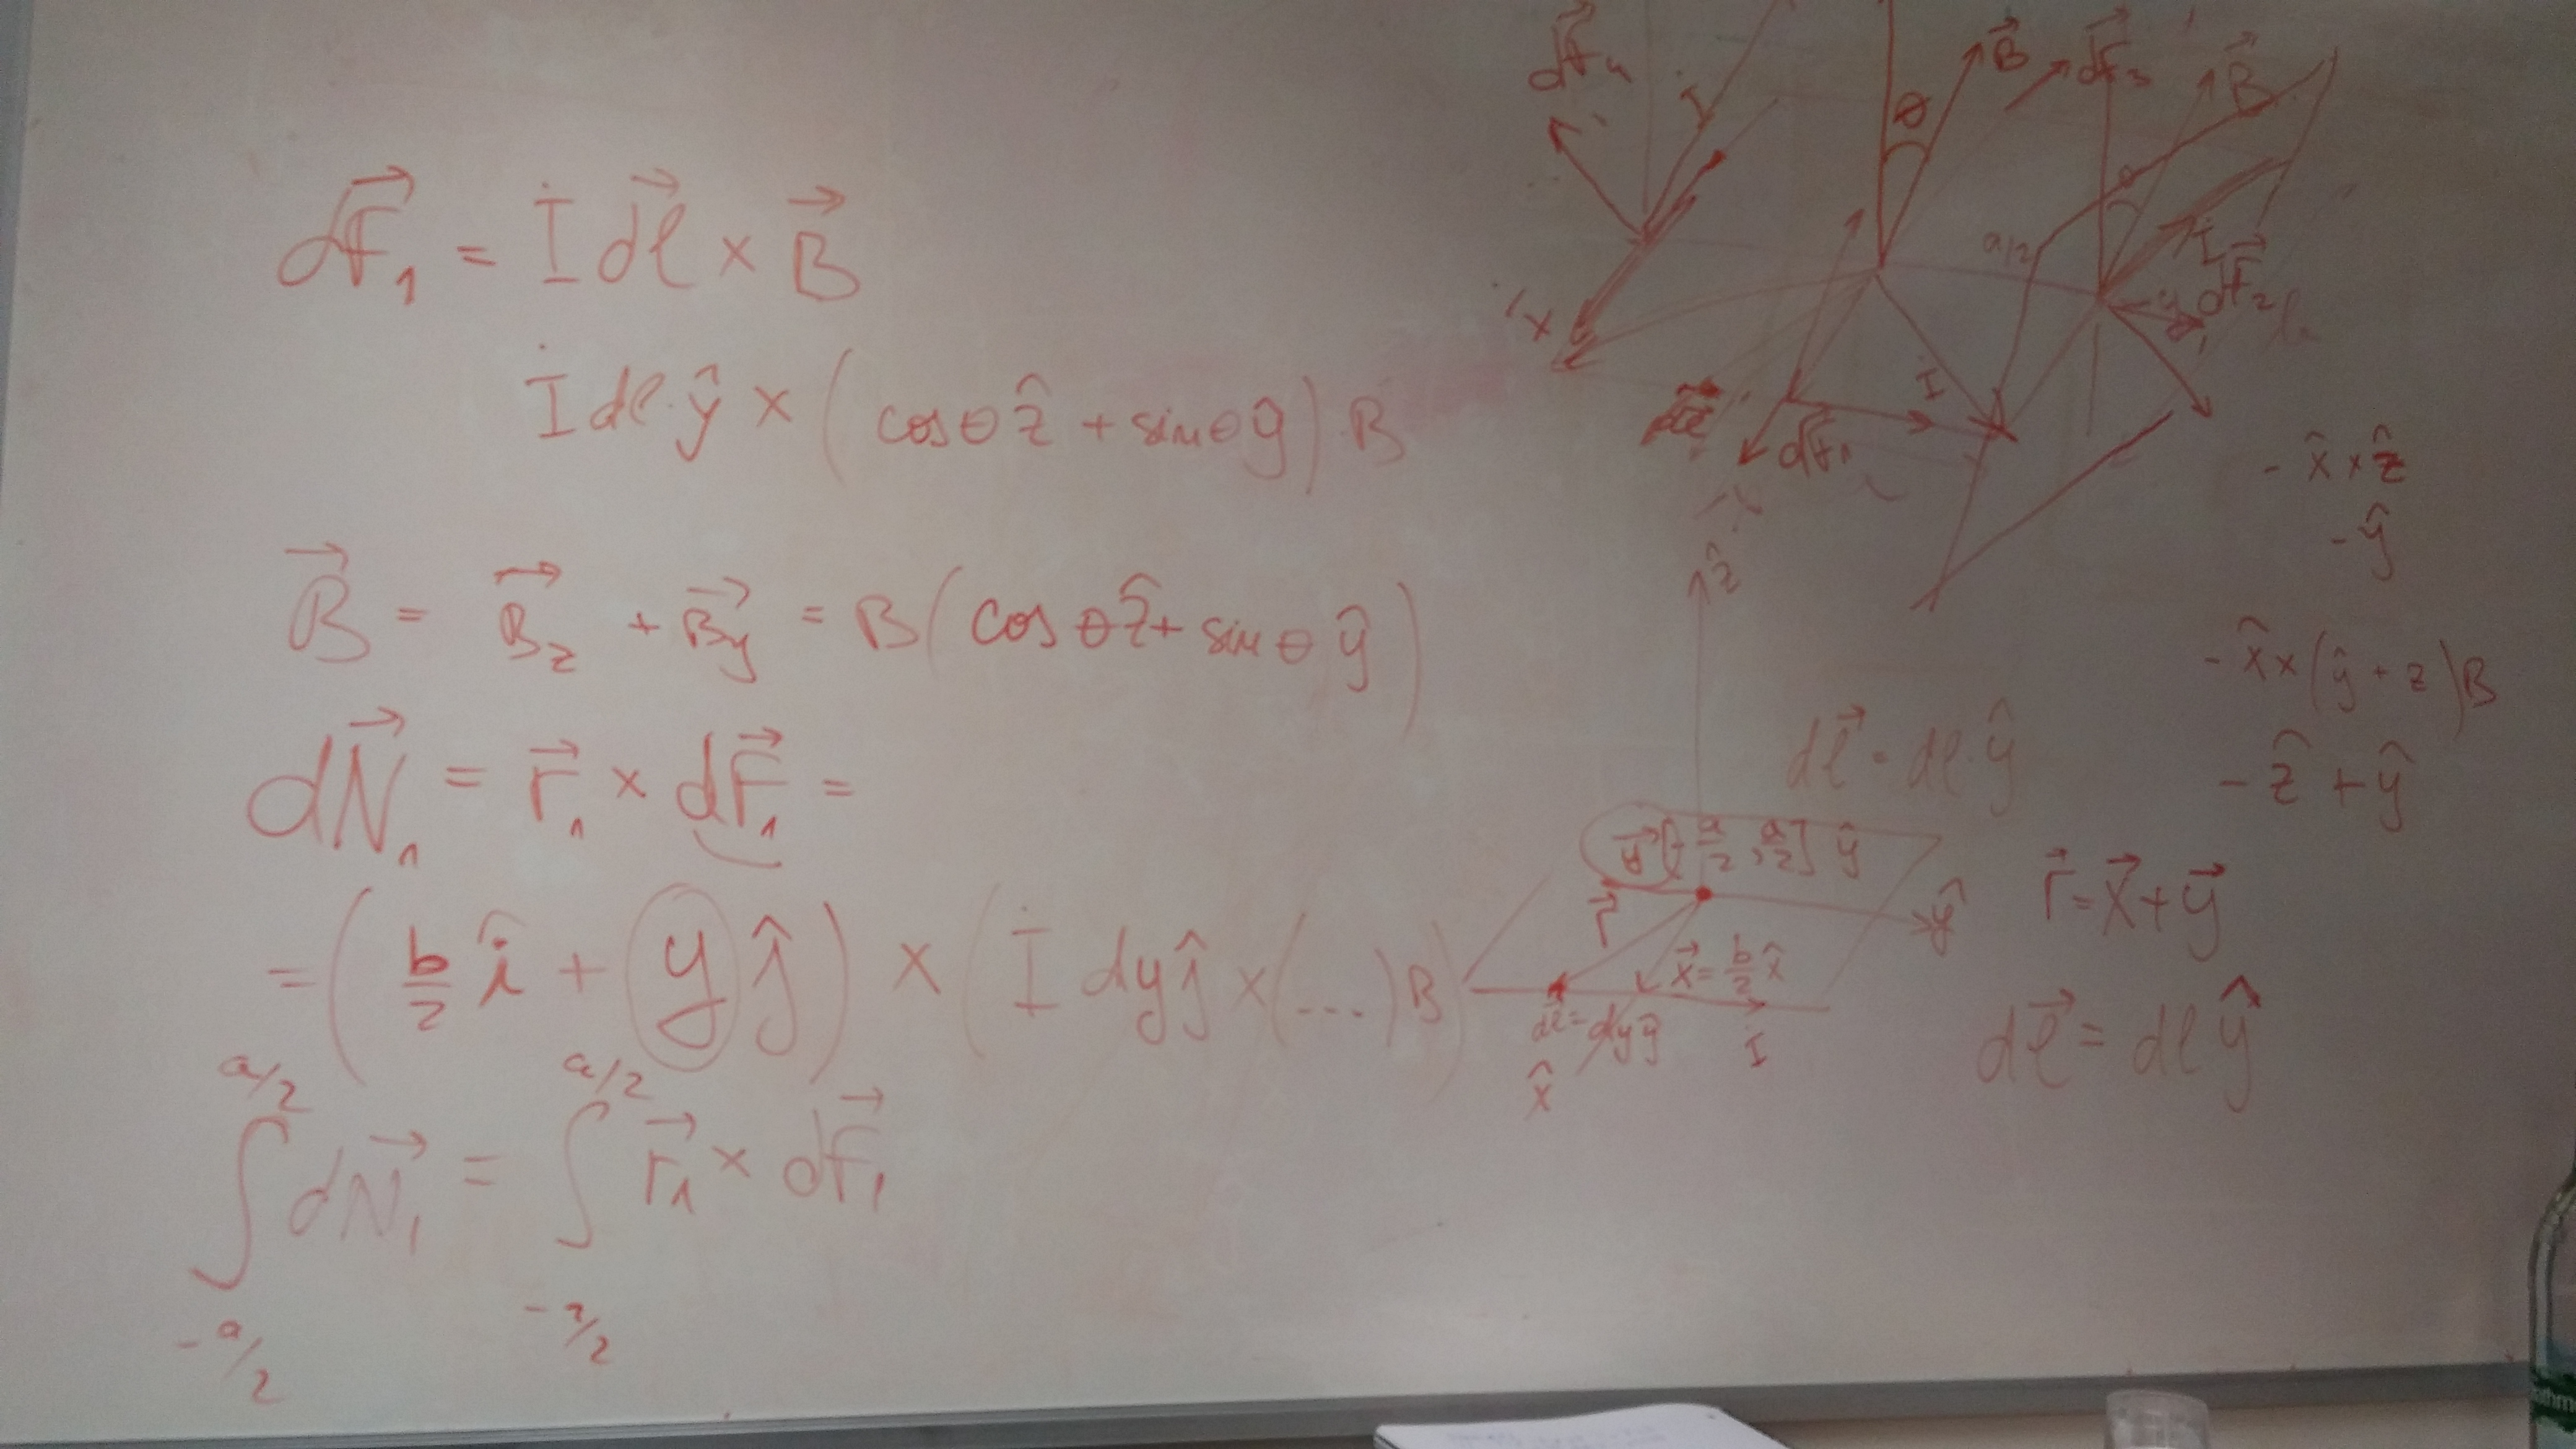
\includegraphics[width=0.8\textwidth,keepaspectratio]{Ch2Gary2}
%    \label{fig:Ch2Gary2}
%\end{figure}
%
%\begin{figure}[H]
%    \centering
%    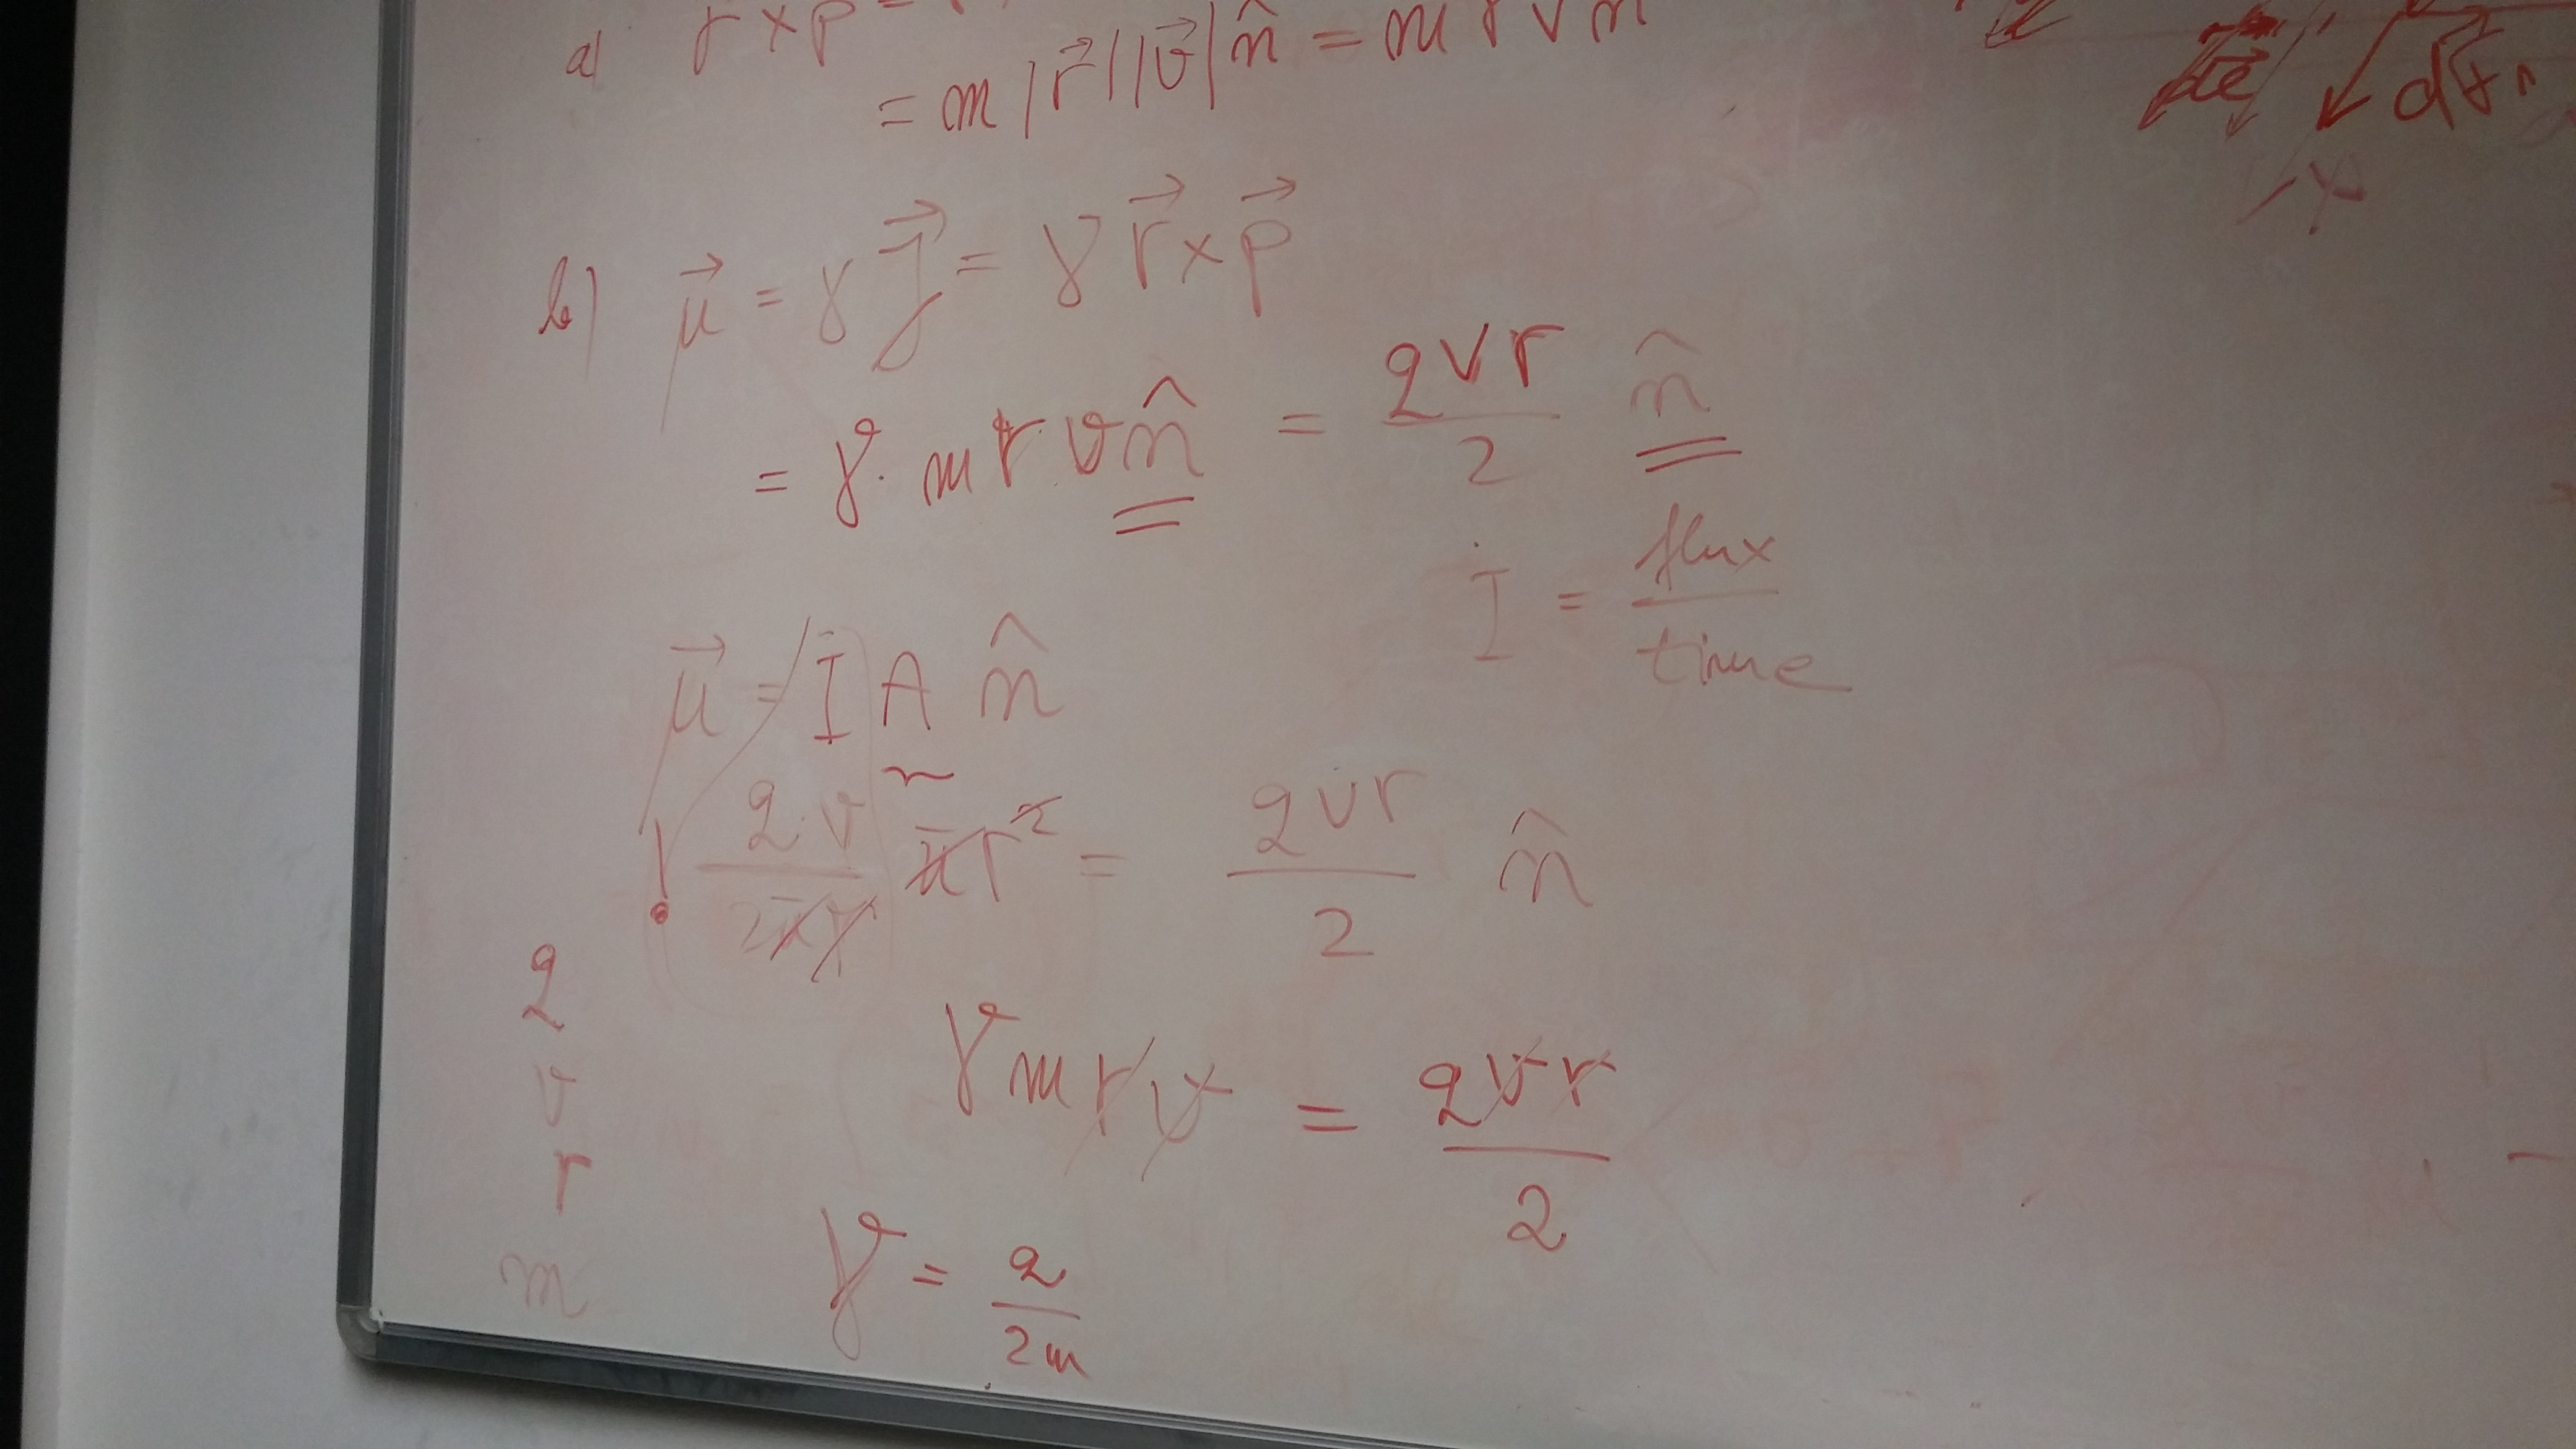
\includegraphics[width=0.8\textwidth,keepaspectratio]{Ch2Gary3}
%    \label{fig:Ch2Gary3}
%\end{figure}
%
%\begin{figure}[H]
%    \centering
%    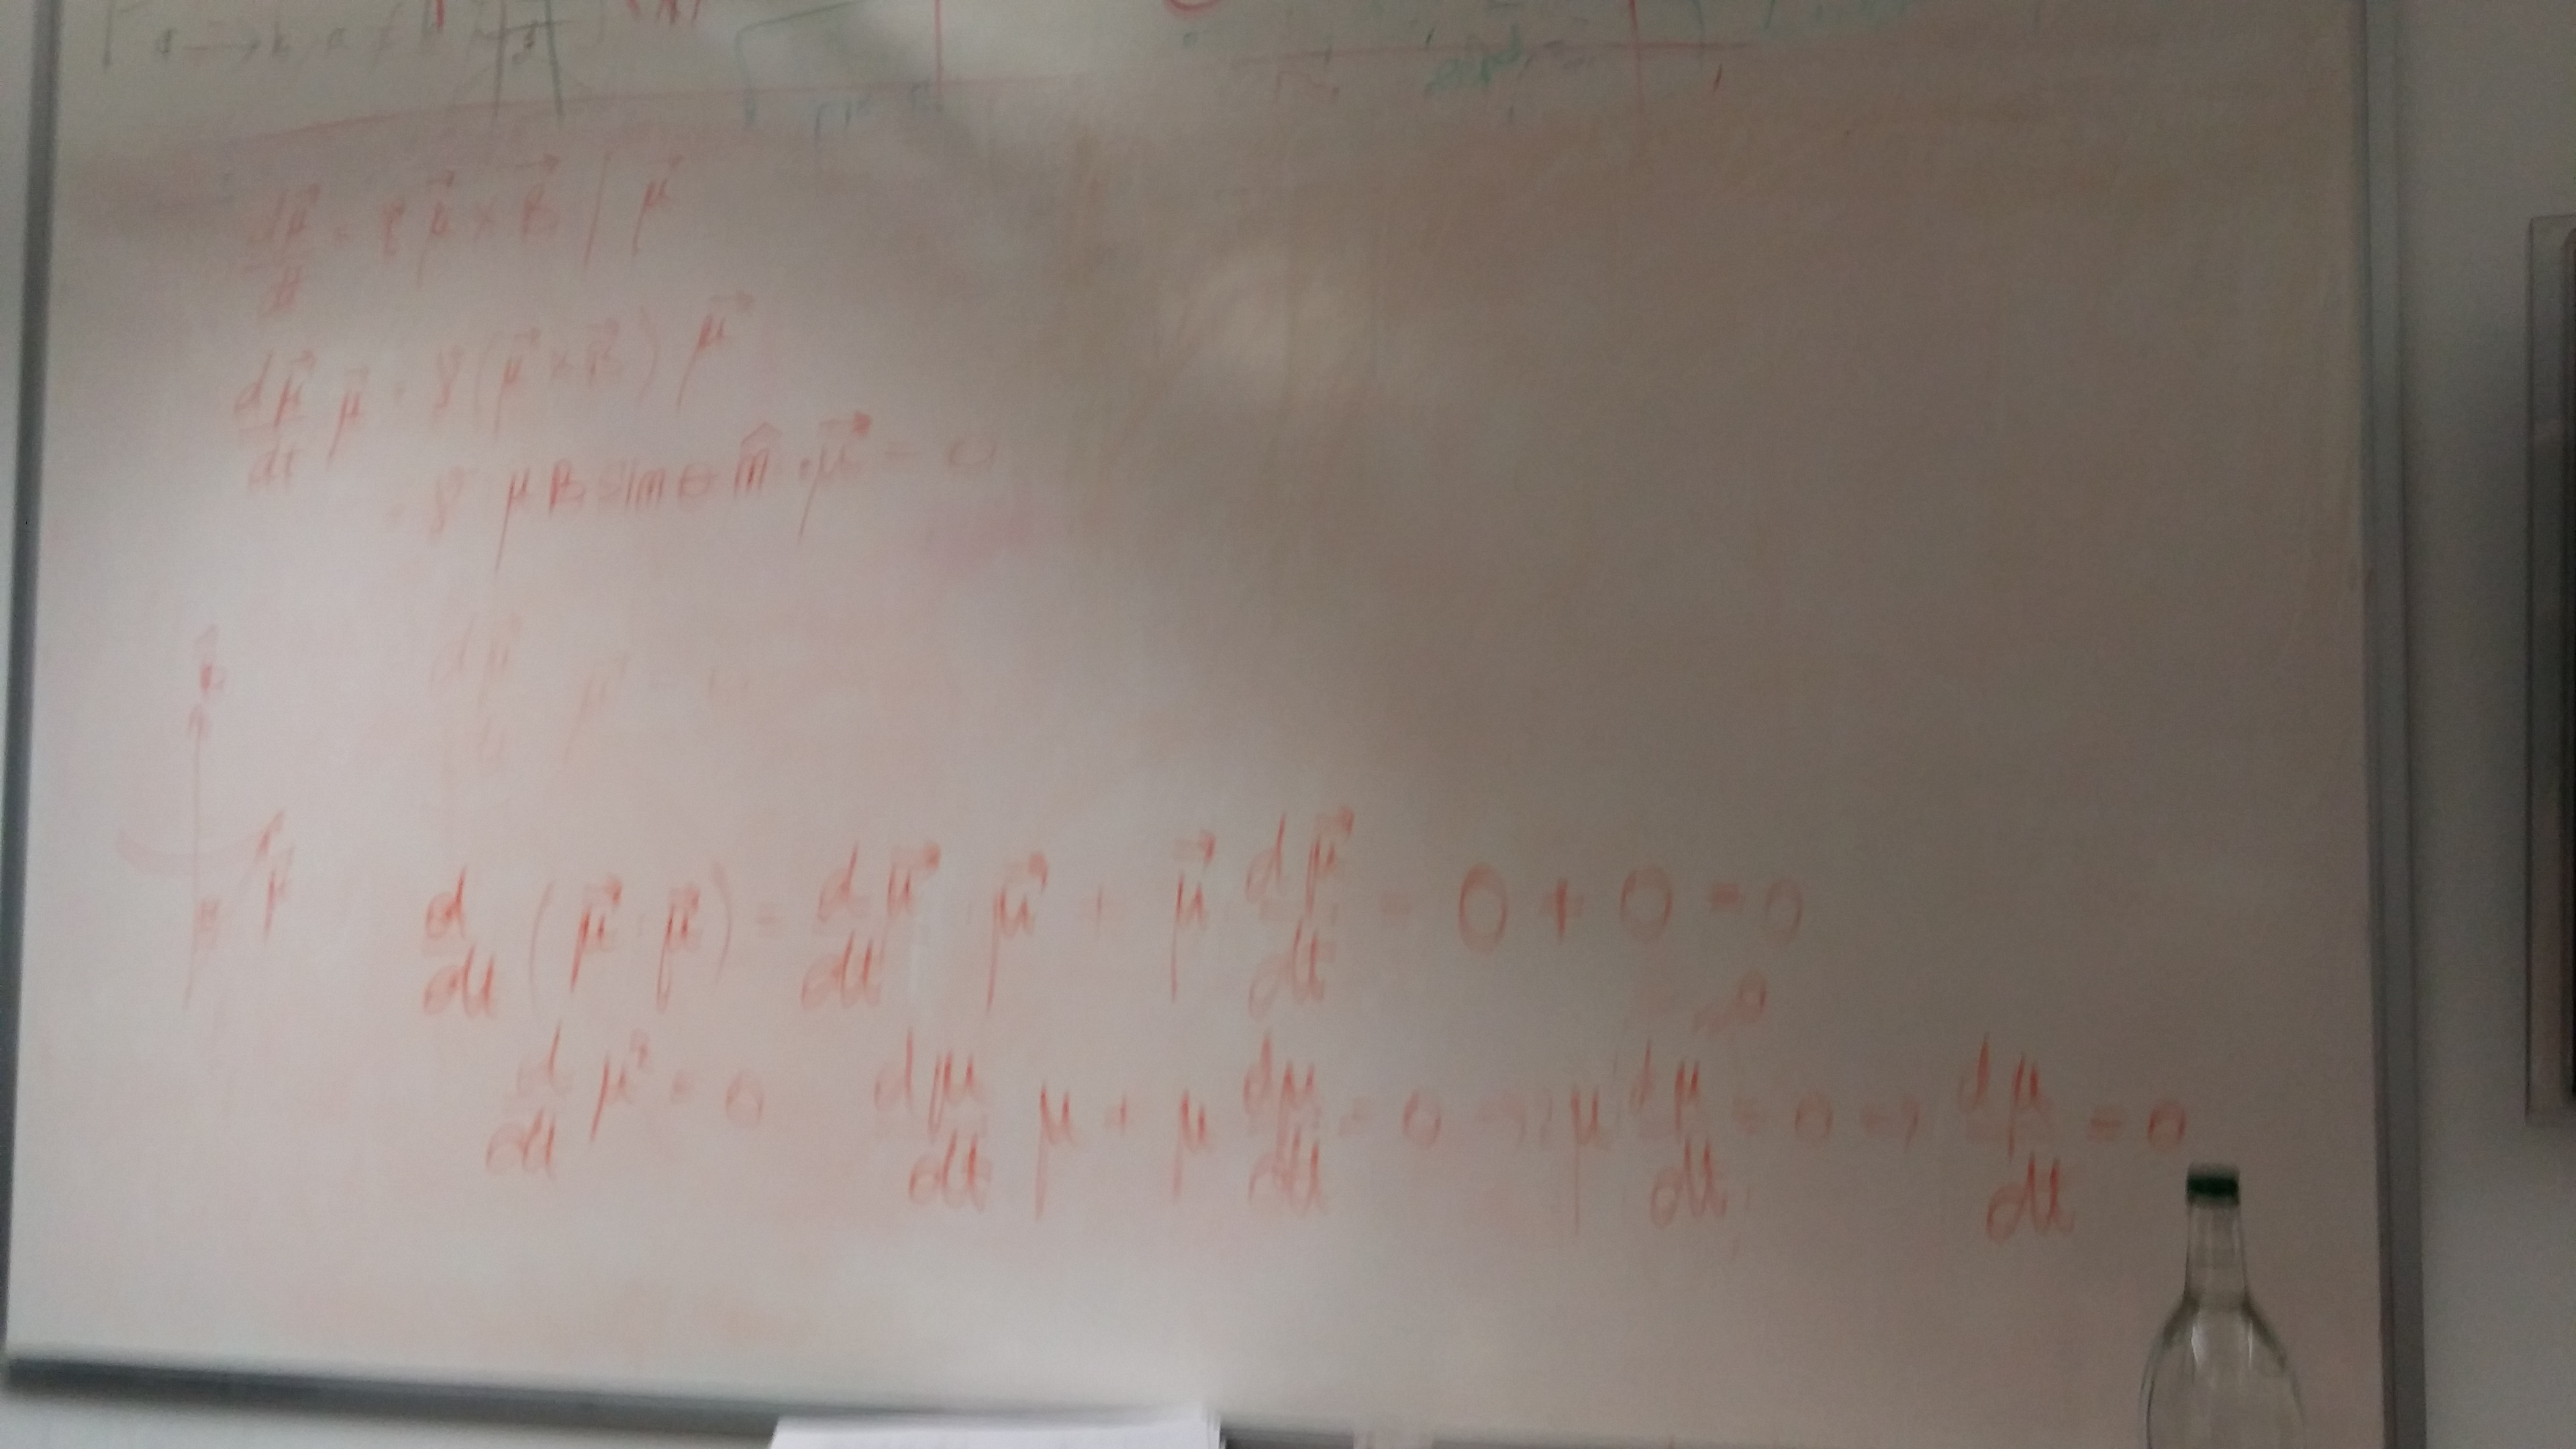
\includegraphics[width=0.8\textwidth,keepaspectratio]{Ch2Gary4}
%    \label{fig:Ch2Gary4}
%\end{figure}
%
%\begin{figure}[H]
%    \centering
%    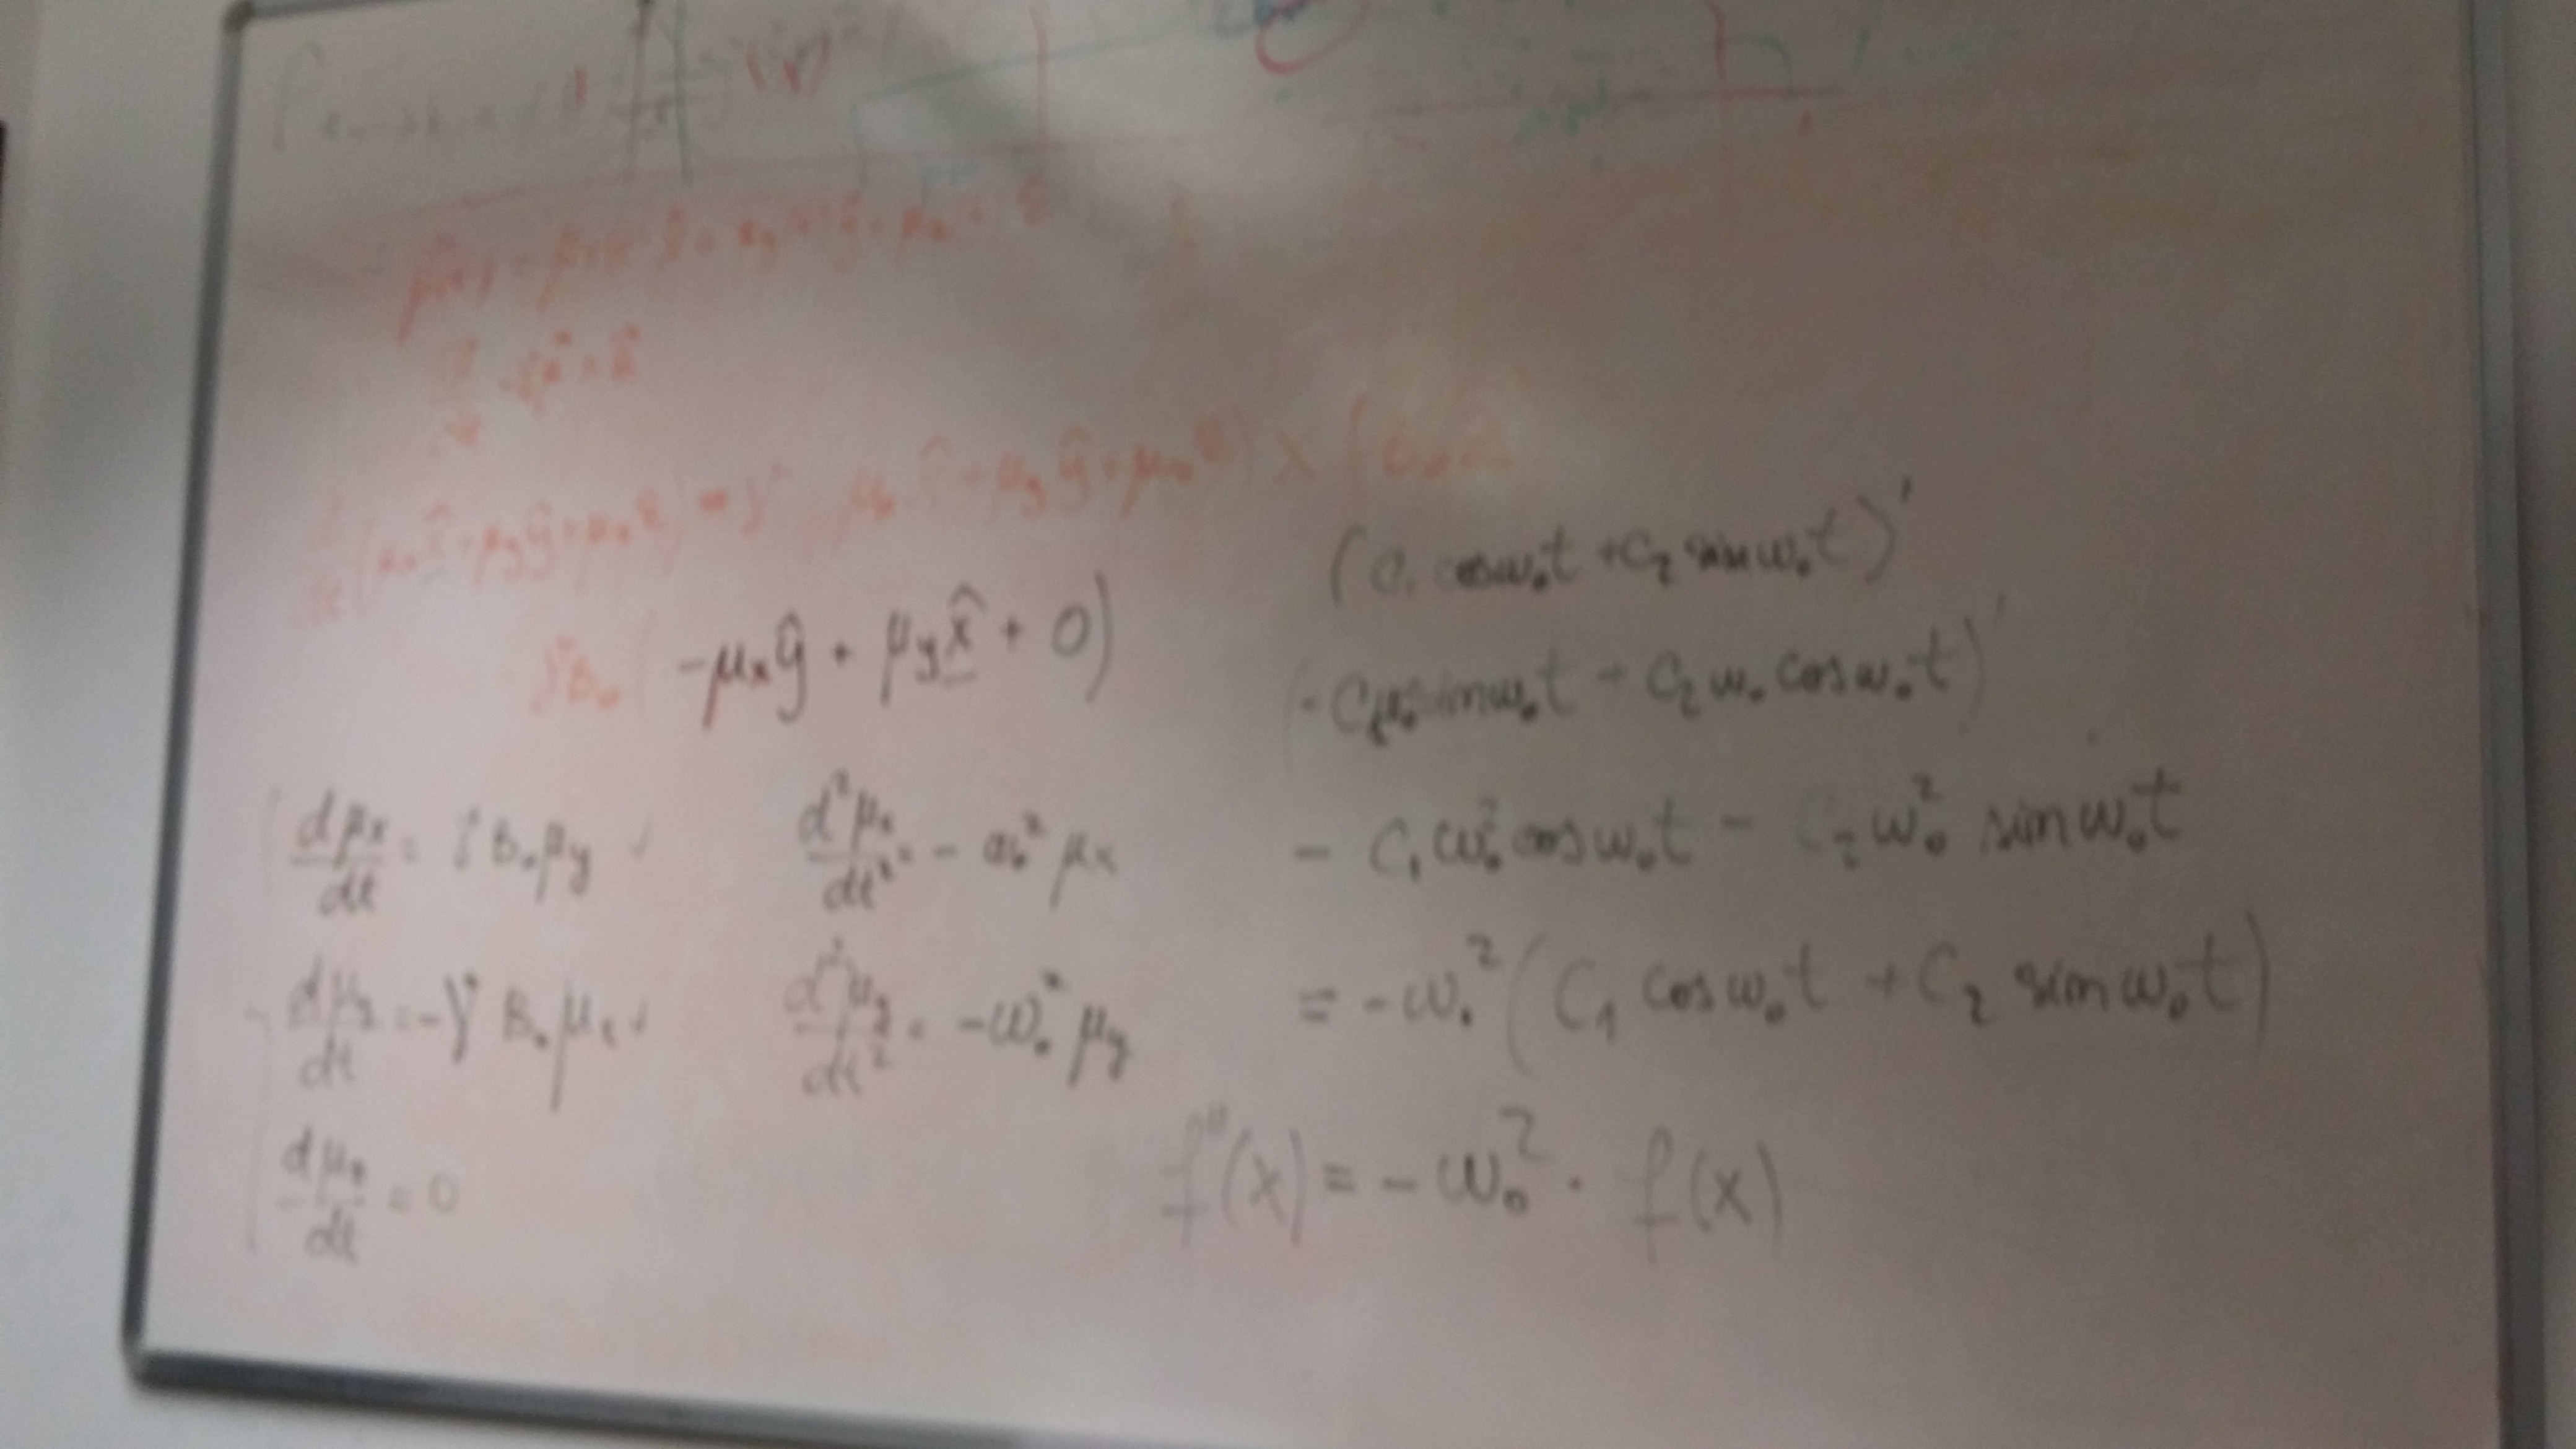
\includegraphics[width=0.8\textwidth,keepaspectratio]{Ch2Gary5}
%    \label{fig:Ch2Gary5}
%\end{figure}
%
%\begin{figure}[H]
%    \centering
%    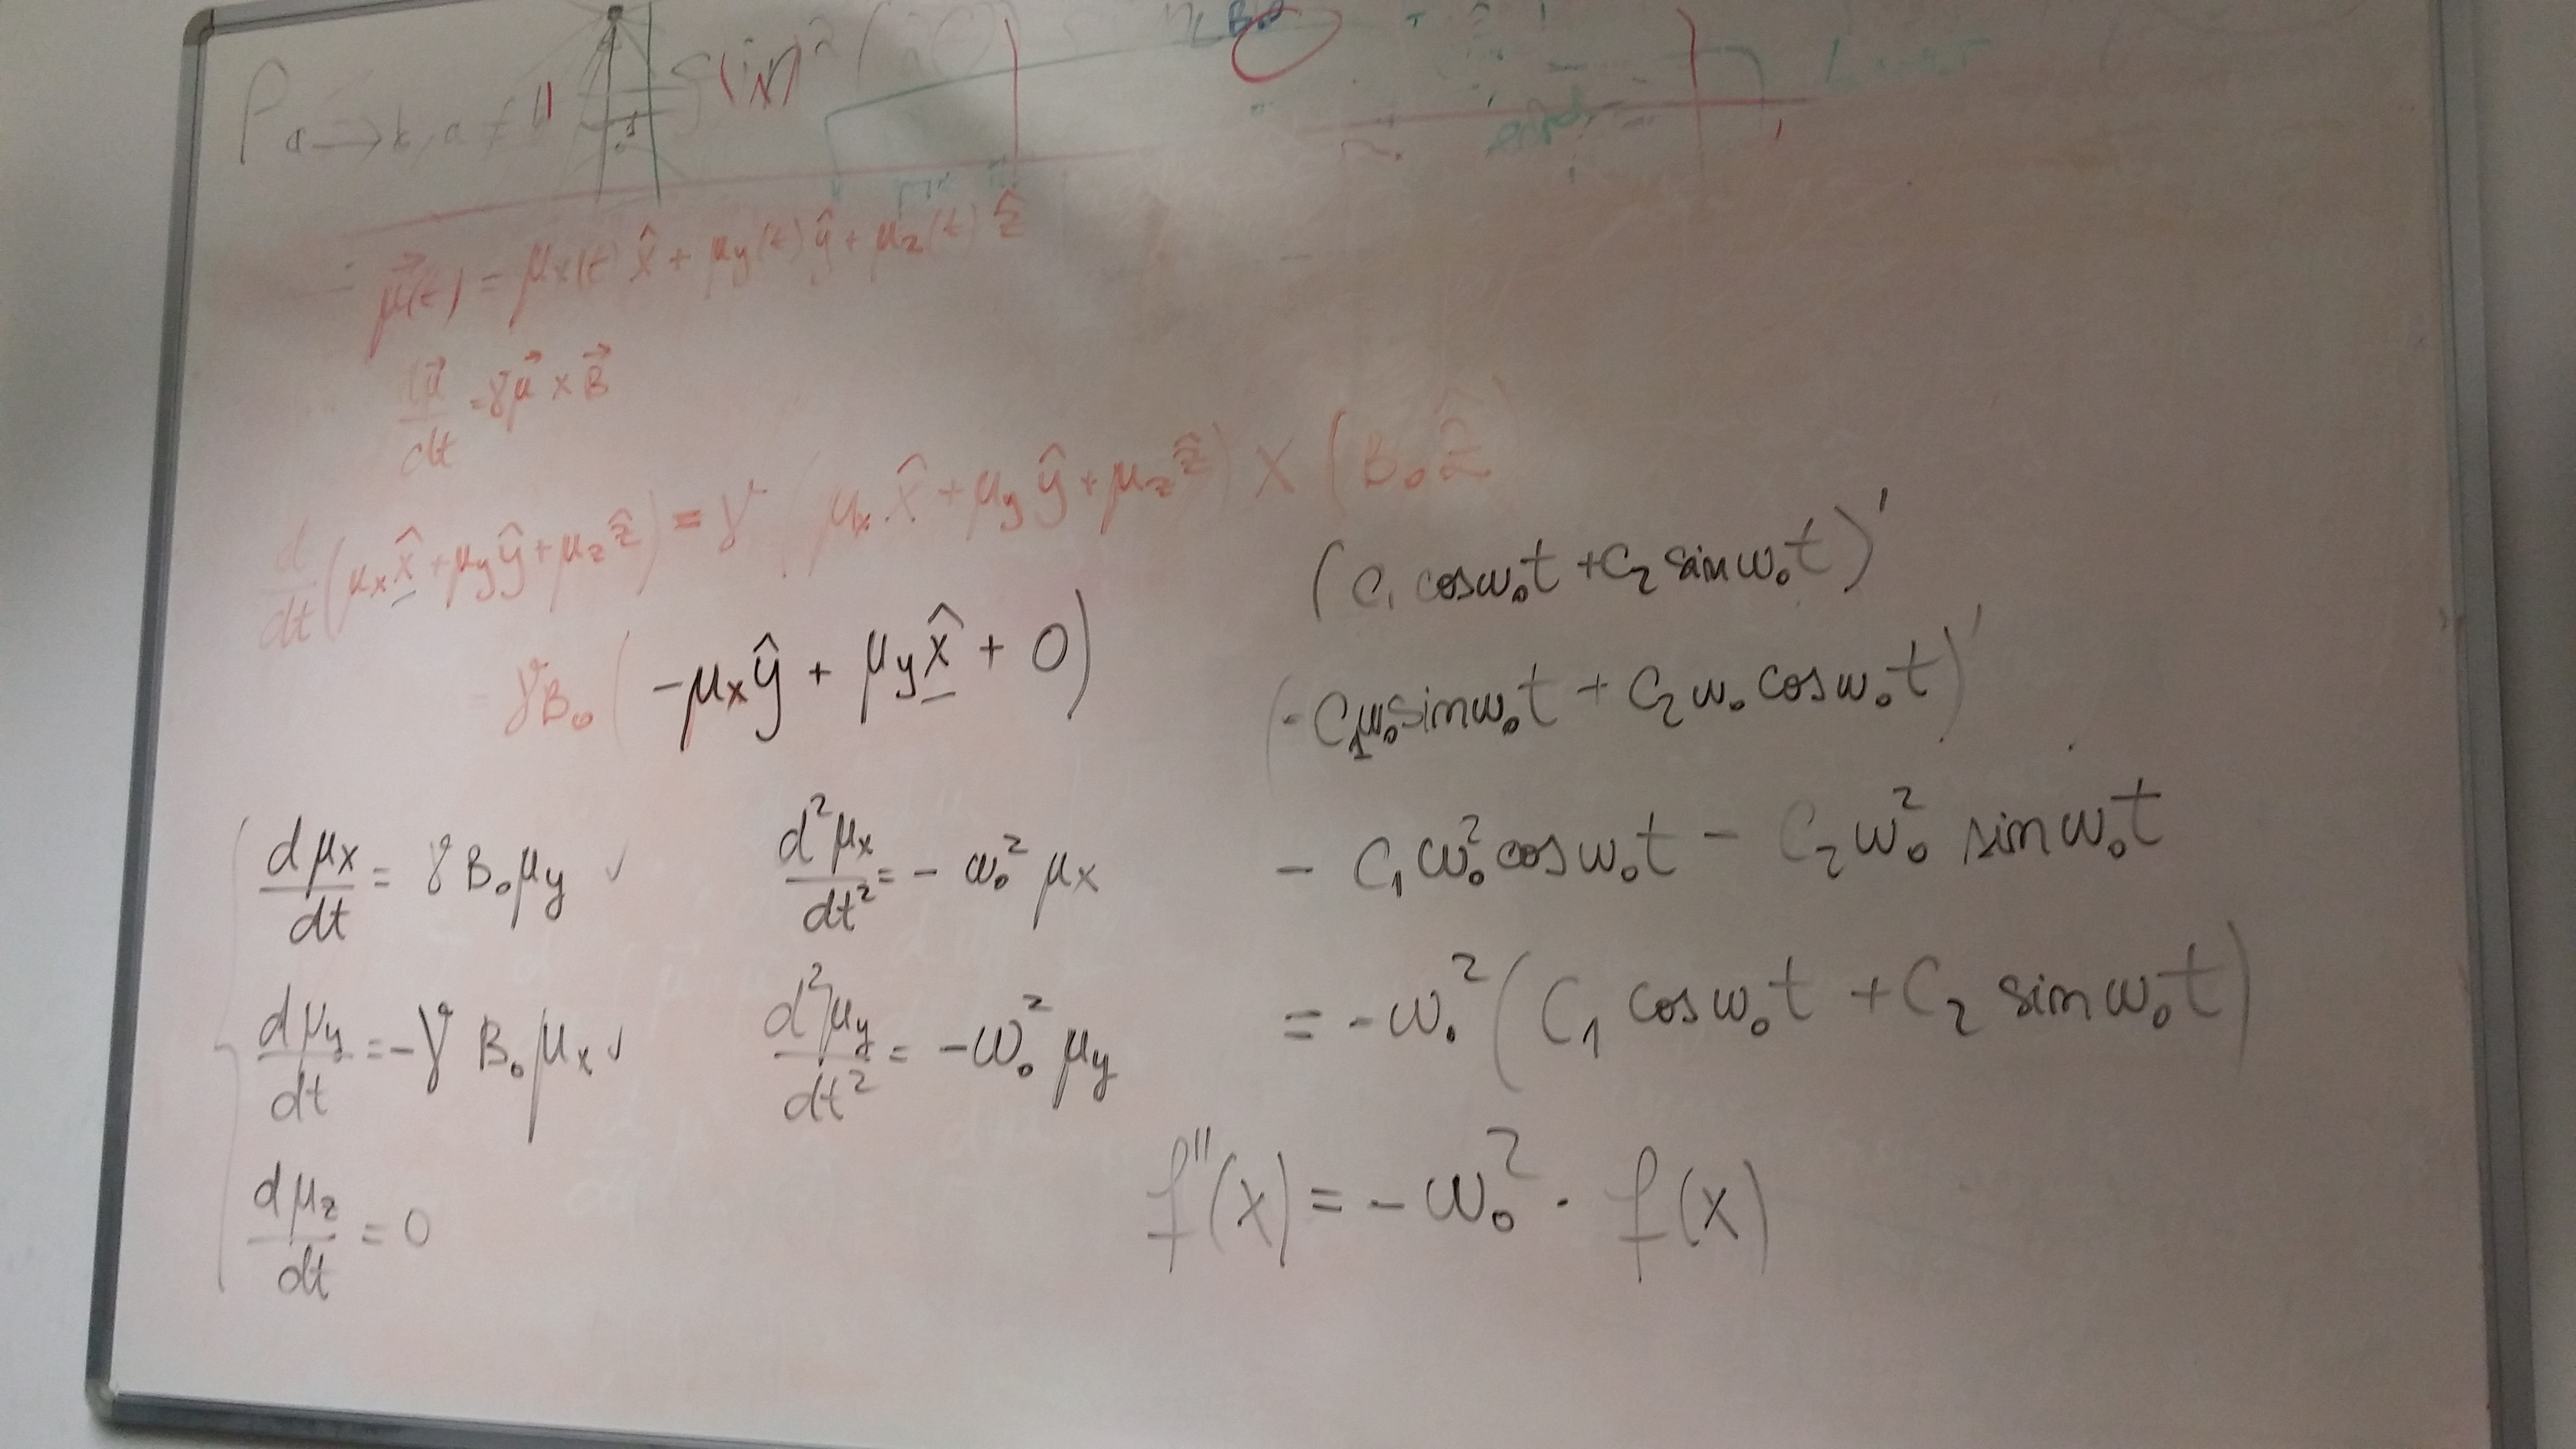
\includegraphics[width=0.8\textwidth,keepaspectratio]{Ch2Gary6}
%    \label{fig:Ch2Gary6}
%\end{figure}
%
%\begin{figure}[H]
%    \centering
%    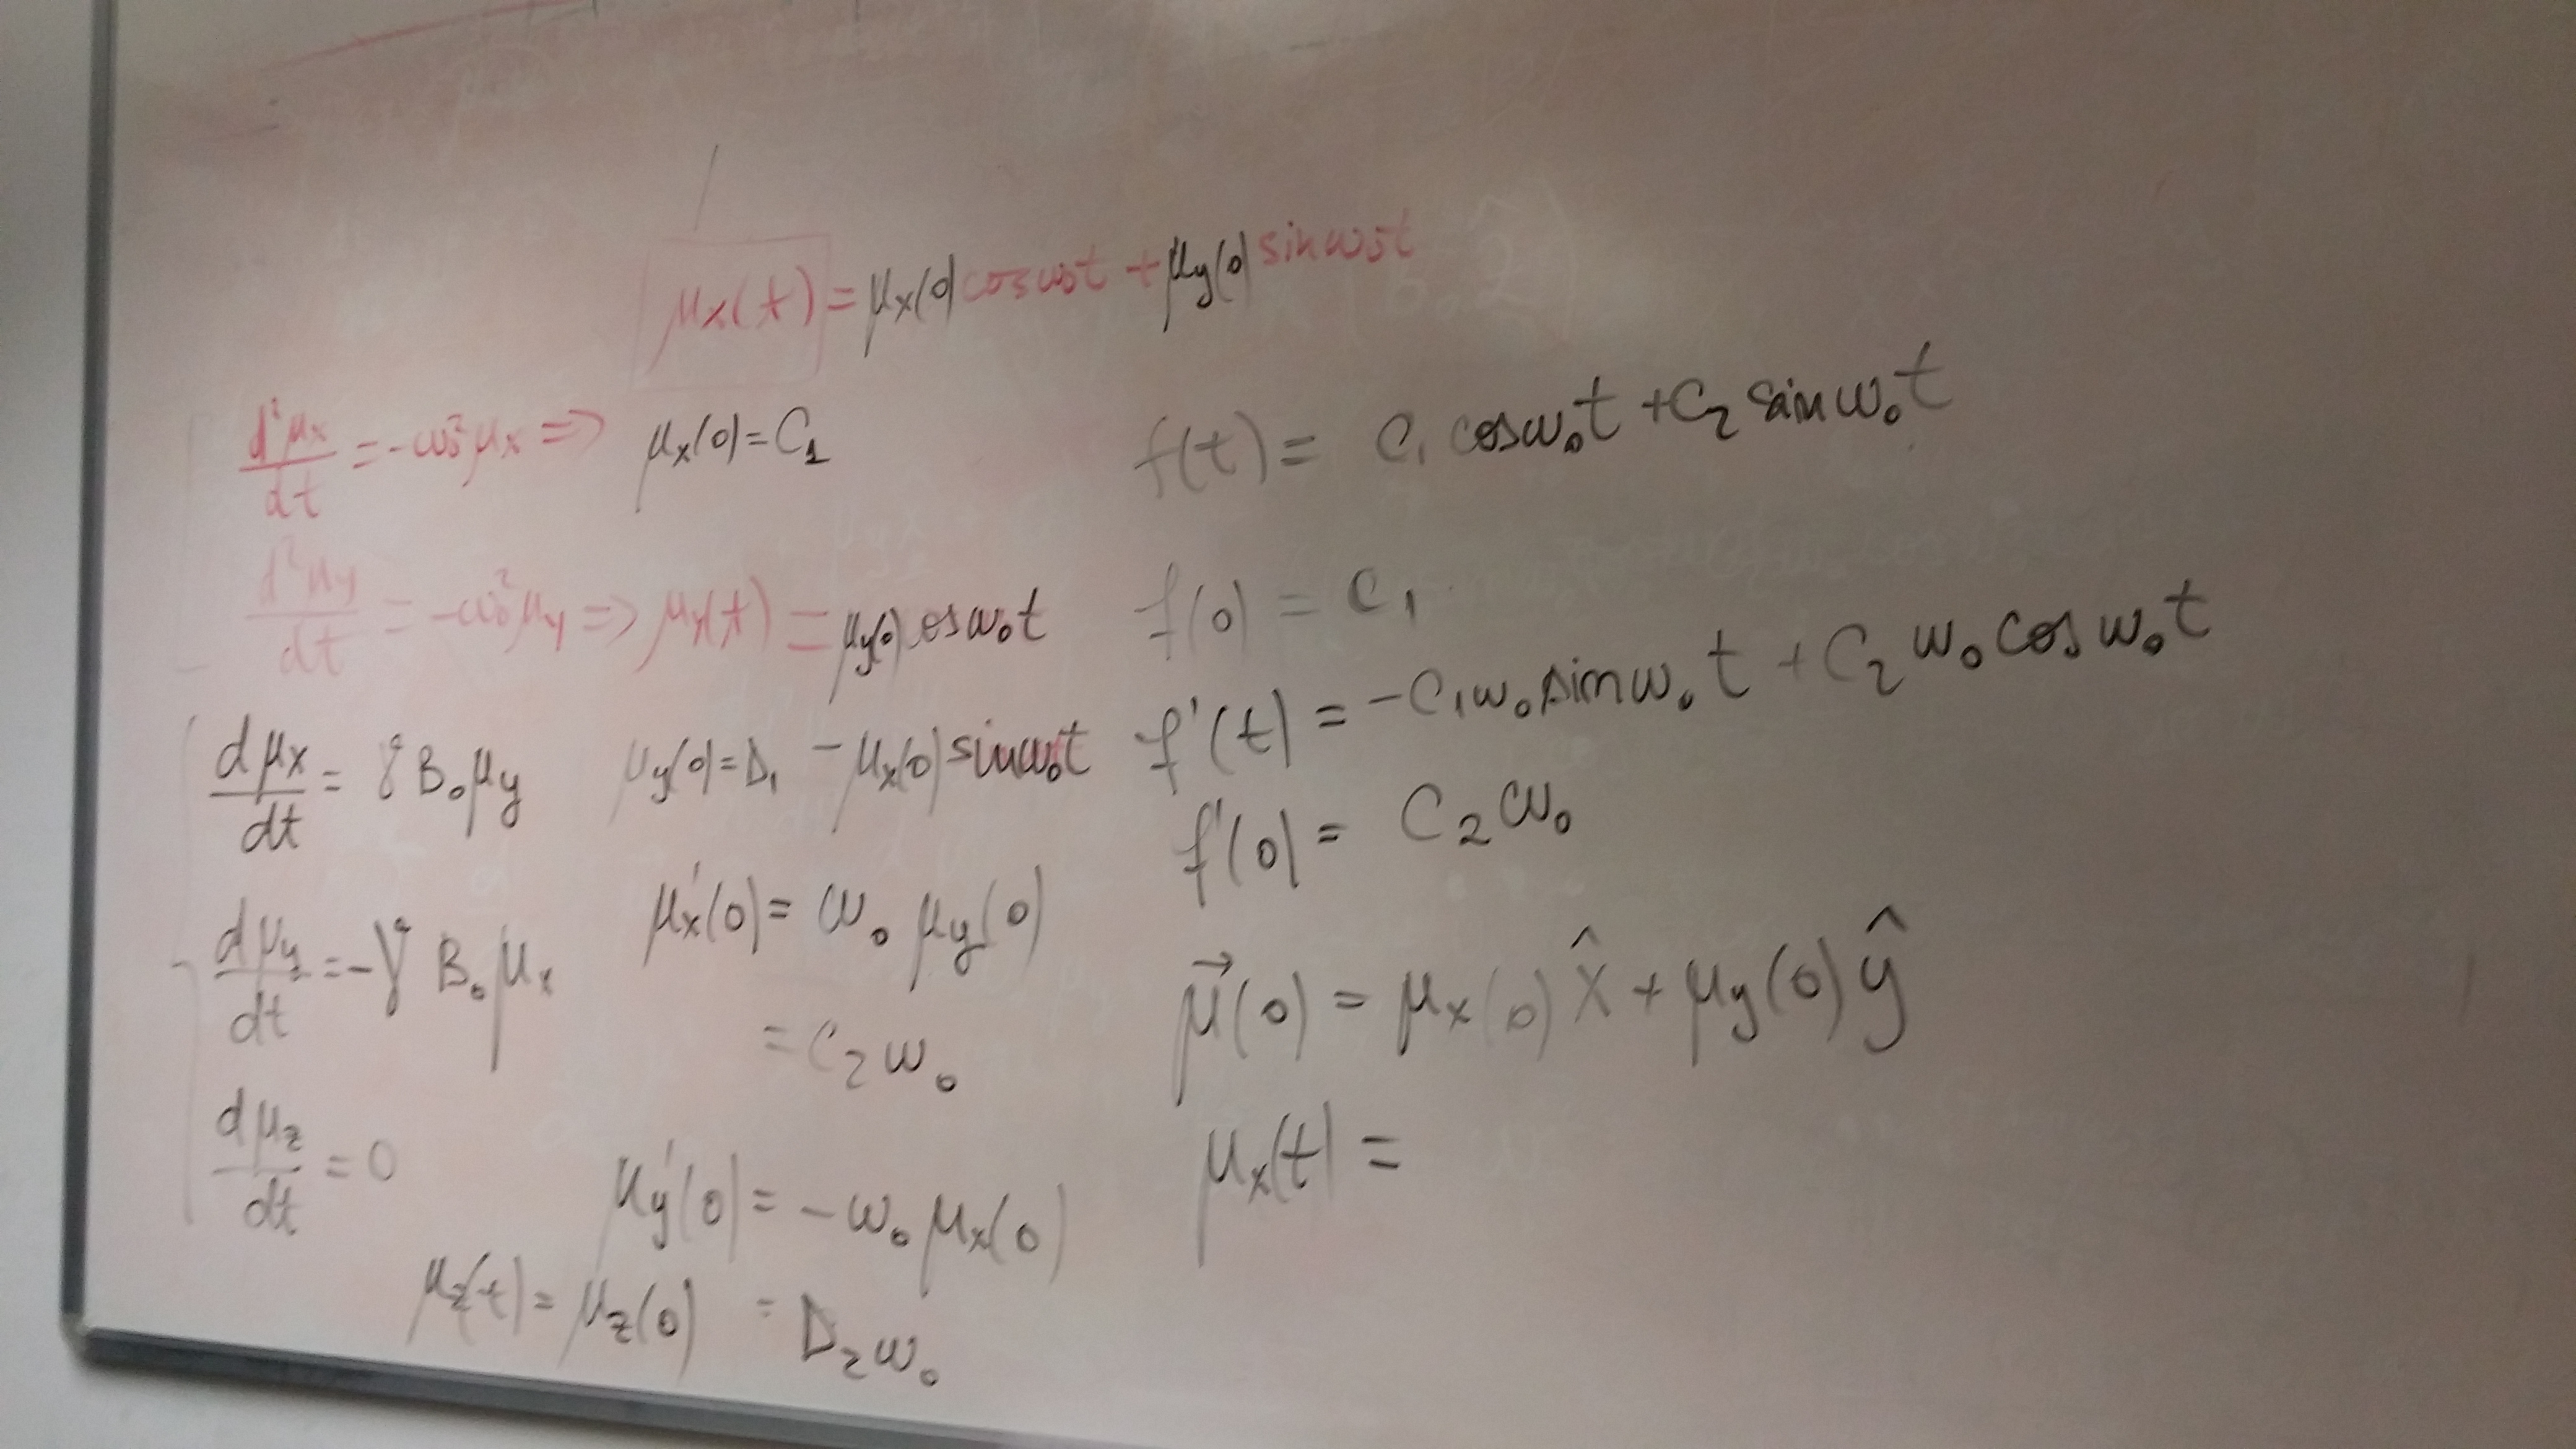
\includegraphics[width=0.8\textwidth,keepaspectratio]{Ch2Gary7}
%    \label{fig:Ch2Gary7}
%\end{figure}
%













\clearpage

%%%%%%%%%%%%%%%%%%%%%%%%%%%%%%
%% CHAPTER 3
%%%%%%%%%%%%%%%%%%%%%%%%%%%%%%
\newpage
\section{Rotating Reference Frames and Resonance}

\subsection{Summary}
\begin{enumerate}
    \item This chapter investigates the response of a spin immersed in a static magnetic field and an additional osciallating magnetic field (going beyond static magnetic field).

\end{enumerate}
\clearpage
%%%%%%%%%%%%%%%%%%%%%%%%%%%%%%
%% EXERCISES
\newpage
\subsection{Exercises}

%%%%%%%%%%%%%%%%%%%%%%%%%%%%%%
\Large{Problem 3.1}
\begin{figure}[H]
    \centering
    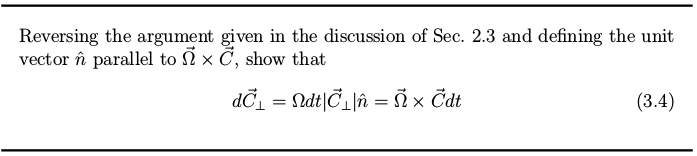
\includegraphics[width=0.8\textwidth,keepaspectratio]{prbl31}
    \label{fig:prbl31}
\end{figure}

\textit{Remember:}
\begin{itemize}
	\item The perpendicular component (perpendicular to $\vec{\Omega}$, 
	the rotational angular velocity vector of the rotating frame) of some vector $\vec{C}$ at rest in 
	the rotating frame has a differential change whose magnitude can 
	be calculated.
	\item The parallel component does not change through time.
    \item $\vec{\Omega} \times \vec{C} $ = anti-clockwise rotation 
\end{itemize}

\textit{Proof.}
\begin{flalign*}
    \frac{d\vec{C}}{dt} &= \vec{\Omega} \times \vec{C} \\
    \frac{d(\vec{C}_{\perp} + \vec{C}_{\|})}{dt} &= \vec{\Omega} \times (\vec{C}_{\perp} + \vec{C}_{\|}) \\
    \frac{d\vec{C}_{\perp}}{dt} + \frac{d\vec{C}_{\|}}{dt} &= \vec{\Omega} \times \vec{C}_{\perp} + \vec{\Omega} \times \vec{C}_{\|} \\
    \frac{d\vec{C}_{\|}}{dt} &= \vec{\Omega} \times \vec{C}_{\|} \\
                             &= \Omega \, \lvert \vec{C_{\|}} \rvert \, sin \,
    0^o \, \hat{n} = \mathbf{0} \\
                             & \Rightarrow \\
    \frac{d\vec{C}_{\perp}}{dt} &= \vec{\Omega} \times \vec{C}_{\perp} \\
    d\vec{C}_{\perp} &= \Omega\, dt \lvert\vec{C}_{\perp}\rvert\, sin \theta\, \hat{n} \\
    \text{But} \, \theta = 90^o &\Rightarrow sin \, \theta = 1 \Rightarrow \\
    d\vec{C}_{\perp} &= \Omega\, dt \lvert\vec{C}_{\perp}\rvert\, \hat{n}
\end{flalign*}

\clearpage
%%%%%%%%%%%%%%%%%%%%%%%%%%%%%%
\Large{Problem 3.2}
\begin{figure}[H]
    \centering
    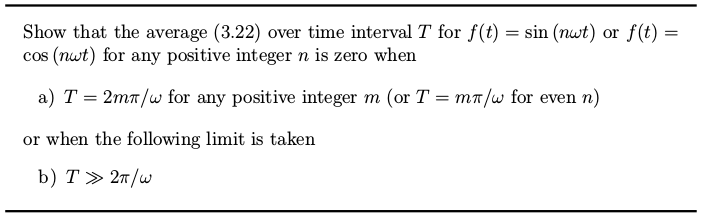
\includegraphics[width=0.8\textwidth,keepaspectratio]{prbl32}
    \label{fig:prbl32}
\end{figure}

\textit{Remember:}
\begin{itemize}
	\item In the rotating reference frame, only half of the original 
	linearly polarized field ($\vec{B_1}^{lin} = b_1^{lin} \, cos \, 
	(\omega t) \, \hat{x}$) is available to tip the spin ($\vec{B_1}^{lin} = 
	\frac{1}{2} \, b_1^{lin} [\hat{x}' (1 + cos \, 2 \omega t) + 
	\hat{y}' sin \, 2 \omega t]$).
	\item The idea is that the effects of the oscillating terms 
	average to zero over times that are half multiples of the rf 
	period, or for all times large compared to the rf period.
\end{itemize}

\textit{Also remember:}
\begin{align*}
    \int_{0}^{2 \pi} sin(x) dx = 0 \\
    \int_{0}^{2 \pi} cos(x) dx = 0 \\ 
    \int_{\frac{- \pi}{2}}^{\frac{\pi}{2}} cos(x) dx = 2 \\
    \int_{0}^{\pi} sin(x) dx = 2 
\end{align*}

\textit{a) Proof.}
\begin{flalign*}
    <f(t)>\, \equiv \frac{1}{T} \int_0^T f(t) dt &= \frac{1}{T} \int_0^T sin(n\omega t) dt \\
                                 &= \frac{\omega}{2m\pi} \int_0^{\frac{2m\pi}{\omega}} sin(n\omega t) dt \\
                                 &= \frac{\omega}{2m\pi} [-cos(n \omega t) \frac{1}{n\omega}]_{0}^{\frac{2m\pi}{\omega}} \\
                                 &= \frac{1}{2nm\pi} (-cos(2nm\pi) + cos(0)) \\ 
                                 &= \frac{1}{2nm\pi} - \frac{1}{2nm\pi} cos(2nm\pi) \\
    \text{We know that: } cos(2N\pi) &= 1 \text{ for } N \in \mathbb{Z} \Rightarrow \\
    \frac{1}{T} \int_0^T f(t) dt &= 0 
\end{flalign*}

\textit{b) Proof.}
\begin{flalign*}
    <f(t)>\, \equiv \frac{1}{T} \int_0^T f(t) dt &= \frac{1}{T} \int_0^T sin(n\omega t) dt \\
                                                 &= \frac{1}{T} [-cos(n\omega t) \frac{1}{n \omega}]_{0}^{T} \\
                                 &= \frac{1}{n \omega T} (- cos(n \omega T) + cos(0)) \\
                                 &= \frac{1}{n \omega T} (1 - cos(n \omega T)) \\
\end{flalign*}



%\begin{figure}[H]
%    \centering
%    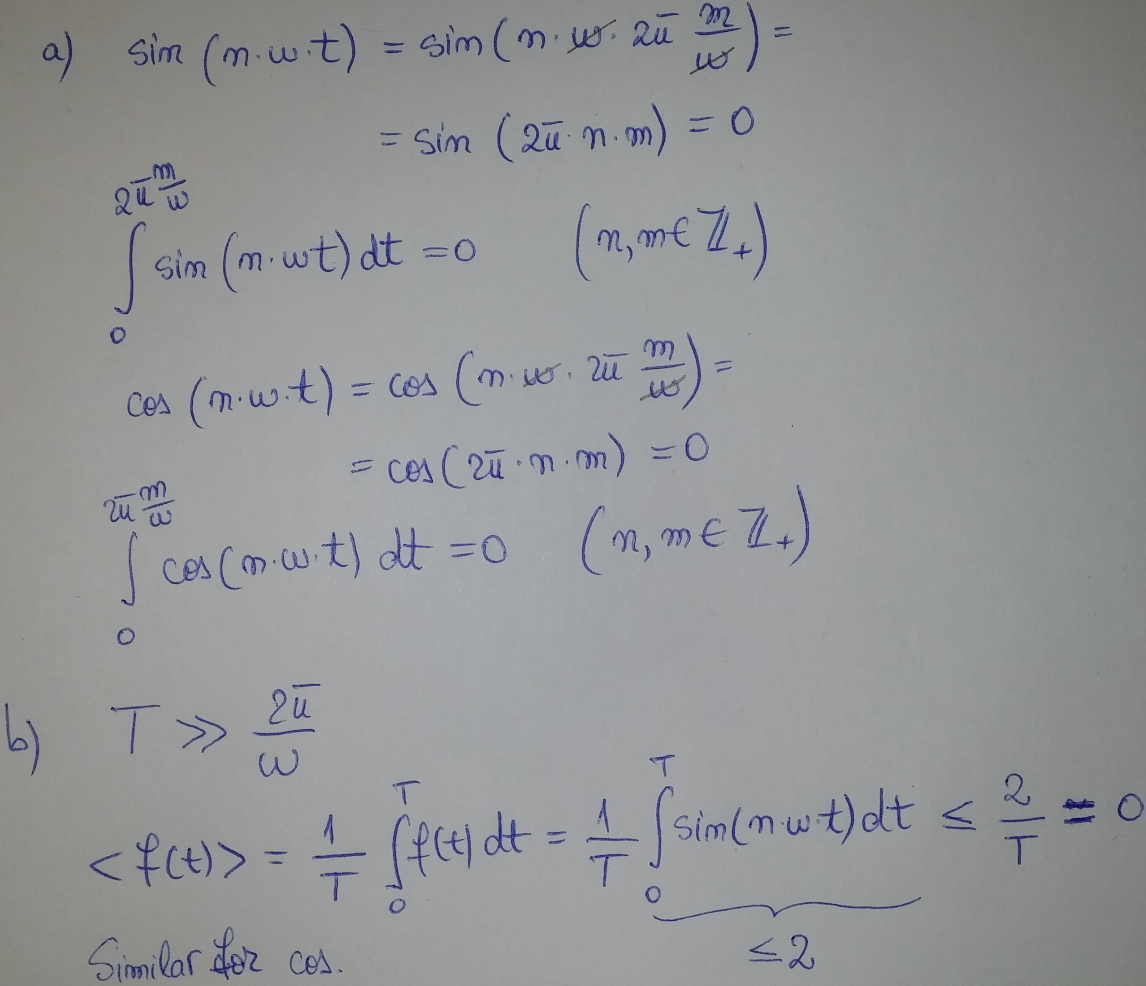
\includegraphics[width=0.8\textwidth,keepaspectratio]{prbl32s}
%    \label{fig:prbl32s}
%\end{figure}

\clearpage
%%%%%%%%%%%%%%%%%%%%%%%%%%%%%%
\Large{Problem 3.3}
\begin{figure}[H]
    \centering
    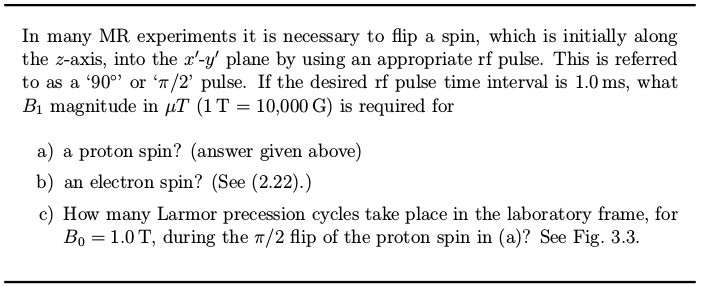
\includegraphics[width=0.8\textwidth,keepaspectratio]{prbl33}
    \label{fig:prbl33}
\end{figure}

\textit{Remember:}
\begin{itemize}
	\item For the same angle of tipping, the rf magnetic field will 
	depend on the type of particle (electron/proton). 
\end{itemize}

\textit{a) Proof.}
\begin{flalign*}
    \Delta \theta &= \gamma_p B_1 \tau \\
    \cancel{\pi} / 2\, \cancel{rad} &= 42.6 \times 10^6 \times 2\cancel{\pi}\, \cancel{rad}\, T^{-1} \cancel{s^{-1}}\, B_1\, 10^{-3} \cancel{s} \\
    B_1 &= \frac{1}{4 \times 42.6} \times 10^{-3}\, T \\ 
    B_1 &= 5.87 \mu T
\end{flalign*}

\textit{b) Proof.}
\begin{flalign*}
    \Delta \theta &= \gamma_e B_1 \tau \\
    \cancel{\pi} / 2\, \cancel{rad} &= 658 \times 42.6 \times 10^6 \times 2\cancel{\pi}\, \cancel{rad}\, T^{-1} \cancel{s^{-1}}\, B_1\, 10^{-3} \cancel{s} \\
    B_1 &= \frac{1}{4 \times 658 \times 42.6} \times 10^{-3}\, T \\ 
    B_1 &= 0.009 \mu T
\end{flalign*}

\textit{c) Proof.}
\begin{flalign*}
    \omega_0 &= \gamma B_0  \\
    \cancel{2\pi\, rad}\, \nu_0 &= 42.6 \times 10^6 \times \cancel{2\pi\, rad}\, \cancel{T^{-1}}\, s^{-1} \times 1\, \cancel{T}\\
    \nu_0 &= 42.6 \, MHz
\end{flalign*}


\clearpage
%%%%%%%%%%%%%%%%%%%%%%%%%%%%%%
\Large{Problem 3.4}
\begin{figure}[H]
    \centering
    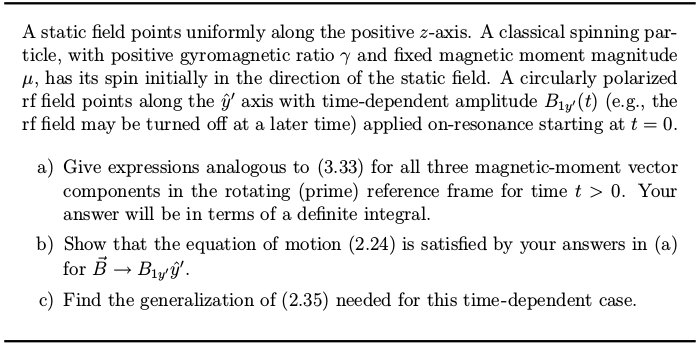
\includegraphics[width=0.8\textwidth,keepaspectratio]{prbl34}
    \label{fig:prbl34}
\end{figure}

\textit{Remember:}
\begin{itemize}
	\item The magnetic moment motion behaves similarly for an 
	on-resonance effective field.
\end{itemize}


\textit{a) You are asked to: } give solutions for the motion through time of the magnetic moment vector components when the $B_1$ field is a circularly polarised rf field pointing along the $\vec{y}'$ axis. \\
\textit{   Proof.}

\begin{figure}[H]
    \centering
    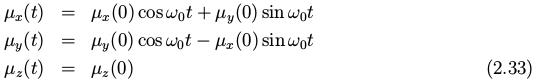
\includegraphics[width=0.7\textwidth,keepaspectratio]{form233}
    \label{fig:form233}
\end{figure}
The total effective field on-resonance will be given by $\vec{B} = B_{1y'}
\hat{y}'$. The magnetic moment vector motion is found by transcribing 
the solution (2.33) according to the substitutions: $z \rightarrow y', 
\, x \rightarrow z', \, y \rightarrow x' $ 
%(\frac{d\vec{\mu}}{dt})' &= \vec{\mu} \, \times [\hat{z}' (\omega_0 - \omega) + \hat{y}' \omega_1]  \\

\begin{flalign*}
    \mu_{x'}(t) &= \mu_{x'}(t_0) \, cos \, \phi_1(t) - \mu_{z'}(t_0) \, sin \, \phi_1(t) \\
    \mu_{y'}(t) &= \mu_{y'}(t_0) \\
    \mu_{z'}(t) &= \mu_{z'}(t_0) \, cos \, \phi_1(t) + \mu_{x'}(t_0) \, sin \, \phi_1(t)\\
    \text{with}: \\
    \phi_1 (t) &= \int_{t_0}^{t} dt' \omega_1(t') \\ 
    \text{in which}: \\
    \omega_1(t) &= \gamma \, B_1(t)
\end{flalign*}


\textit{b) Proof.}

\begin{figure}[H]
    \centering
    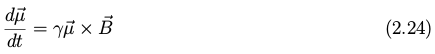
\includegraphics[width=0.6\textwidth,keepaspectratio]{form224}
    \label{fig:form224}
\end{figure}

\begin{flalign*}
    \vec{B}_{1y'}(t) &= B_{1y'} (t) \, \hat{y'} \\
	    			 &= B_{1y'} (t) \, (\hat{x} \, sin \omega t + \hat{y} \, cos \omega 
	    			 t) \\
	\text{We know that:} \\
	(\frac{d\vec{\mu}}{dt})' &= \gamma \vec{\mu}' \times \vec{B}_{1y'}  (t)
	\\
	\frac{d \mu_{x'}(t)}{dt} \hat{x}' + \frac{d \mu_{y'}(t)}{dt} 
	\hat{y}' + \frac{d \mu_{y'}(t)}{dt} \hat{z}' &= \gamma \, 
	(\mu_{x'}(t) \hat{x}' + \mu_{y'}(t) \hat{y}' + \mu_{z'}(t) 
	\hat{z}') \times B_{1y'} (t) \hat{y}' \\
	&= \gamma B_{1y'} (t) \, ( \mu_{x'}(t) \hat{x}' \times \hat{y}' + 
	\mu_{y'}(t) \hat{y}' \times \hat{y}' + \mu_{z'}(t) \hat{z}' \times 
	\hat{y}') \\
	&= \gamma B_{1y'} (t) \, ( \mu_{x'}(t) \hat{z}' - \mu_{z'}(t) \hat{x}' 
	)  \\
	\Rightarrow \\
	\frac{d \mu_{x'}(t)}{dt} &= - \gamma \mu_{z'}(t) B_{1y'} (t) = - 
	\omega_1 (t) \mu_{z'}(t) \\
	\frac{d \mu_{y'}(t)}{dt} &= 0 \\
	\frac{d \mu_{z'}(t)}{dt} &= \gamma \mu_{x'}(t) B_{1y'} (t) = 
	\omega_1 (t) \mu_{x'}(t)\\ \\
	\text{Taking the first derivative } & \text{of the solutions from 
	a) we get}: \\
	\frac{d \mu_{x'}(t)}{dt} &= - \, \mu_{x'}(t_0) \, \omega_1(t) \, sin \, 
	\phi_1(t) \, - \mu_{z'}(t_0) \, \omega_1(t) \, cos \, 
	\phi_1(t) \\
	&= - \, \omega_1(t) \, (\mu_{x'}(t_0) \, sin \, \phi_1(t) + \mu_{z'}(t_0) \, cos \, 
	\phi_1(t)) \\
	&= - \, \omega_1(t) \, \mu_{z'}(t) \\
	\frac{d \mu_{y'}(t)}{dt} &= 0 \\
	\frac{d \mu_{z'}(t)}{dt} &= - \, \mu_{z'}(t_0) \, \omega_1(t) \, sin \, 
	\phi_1(t) \, + \mu_{x'}(t_0) \, \omega_1(t) \, cos \, 
	\phi_1(t) \\
	&= \omega_1(t) \, (\mu_{x'}(t_0) \, cos \, \phi_1(t) - \mu_{z'}(t_0) 
	\, sin \, 
	\phi_1(t)) \\
	&= \omega_1(t) \, \mu_{x'}(t) \\
\end{flalign*}


\textit{c) Proof.}
\begin{figure}[H]
    \centering
    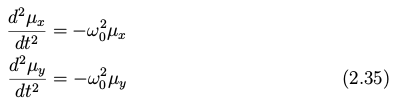
\includegraphics[width=0.6\textwidth,keepaspectratio]{form235}
    \label{fig:form235}
\end{figure}

\begin{flalign*}
	\frac{d^2 \mu_{x'}(t)}{dt^2} &= \frac{d}{dt} \, (\frac{d 
	\mu_{x'}(t)}{dt}) \\
    &= - \frac{d}{dt} \, (\omega_1(t) \mu_{z'}(t)) \\
    &= - \frac{d \omega_1(t)}{dt} \, \mu_{z'}(t) - \omega_1(t) \, \frac{d \mu_{z'}(t)}{dt}  \\
    &= - \frac{d \omega_1(t)}{dt} \, \mu_{z'}(t) - \omega_1^2(t) \mu_{x'}(t)  \\
	\frac{d^2 \mu_{z'}(t)}{dt^2} &= \frac{d}{dt} \, (\frac{d 
	\mu_{z'}(t)}{dt}) \\
	&= \frac{d}{dt} \, (\omega_1(t) \mu_{x'}(t)) \\
    &= \frac{d \omega_1(t)}{dt} \, \mu_{x'}(t) + \omega_1(t) \, \frac{d \mu_{x'}(t)}{dt}  \\
    &= \frac{d \omega_1(t)}{dt} \, \mu_{x'}(t) - \omega_1^2(t) \mu_{z'}(t) 
\end{flalign*}

\clearpage
%%%%%%%%%%%%%%%%%%%%%%%%%%%%%%
\Large{Problem 3.5}
\begin{figure}[H]
    \centering
    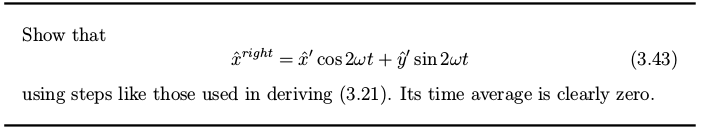
\includegraphics[width=0.8\textwidth,keepaspectratio]{prbl35}
    \label{fig:prbl35}
\end{figure}

\textit{Remember:}
\begin{itemize}
	\item A left-circularly polarized field is maximally effective in 
	tipping the spin around the $x'$-axis, while a right-circularly 
	polarized field is completely ineffective.
\end{itemize}

\textit{Proof.}\\
\textit{We know that:}
\begin{flalign*}
    \hat{x}^{right} &= \hat{x} \, cos \omega t + \hat{y} \, sin \omega t \\
    \hat{x}' &= \hat{x} \, cos \omega t - \hat{y} \, sin \omega t \\
    \hat{y}' &= \hat{x} \, sin \omega t + \hat{y} \, cos \omega t 
\end{flalign*}

\textit{Therefore, we can write:}
\begin{flalign*}
    \hat{x}' \, cos 2\omega t &= \hat{x} \, cos \omega t \, (1 - 2 sin^2 \omega t)  \\
                              &- \hat{y} \, sin \omega t \, (2 \, cos^2 \omega t - 1) \\
                              & = \hat{x} \, cos \omega t - 2 \hat{x} \, cos \omega t\, sin^2 \omega t  \\
                              &- 2 \hat{y}\, sin \omega t \, cos^2 \omega t + \hat{y}\, sin \omega t \\
    \hat{y}' \, sin 2\omega t &= 2 \hat{x} \, sin^2 \omega t\,cos \omega t \\
                              &+ 2 \hat{y}\,sin \omega t\, cos^2 \omega t
\end{flalign*}

\textit{By adding them together we get:}
\begin{flalign*}
    \hat{x}' \, cos 2\omega t + \hat{y}' \, sin 2\omega t &= \hat{x} \, cos \omega t + \hat{y}\, sin \omega t \Rightarrow\\
    \hat{x}' \, cos 2\omega t + \hat{y}' \, sin 2\omega t &= \hat{x}^{right}
\end{flalign*}

\textit{Calculating the time average:}
\begin{flalign*}
    <f(t)> &\equiv \frac{1}{T} \int_{0}^{T} f(t) dt \Rightarrow \\
\end{flalign*}
\begin{flalign*}
    <\hat{x}^{right} > &\equiv \frac{1}{T} \int_{0}^{T} \hat{x}' \, cos 
    2\omega t + \hat{y}' \, sin 2\omega t \, \, dt = \\
    &= \frac{1}{T} \int_{0}^{T} \hat{x} \, cos \omega t + \hat{y} \, sin 
    \omega t \, \, dt \\
\end{flalign*}
\begin{flalign*}
    &= \hat{x} \, \frac{1}{T} \int_{0}^{T} cos \, \omega t \, dt + 
    \hat{y} \, \frac{1}{T} \int_{0}^{T} sin \, \omega t \, dt \, 
    \Rightarrow \text{(as shown in \textit{Problem 3.2})} \\
    &= \mathbf{0}
\end{flalign*}


\clearpage
%%%%%%%%%%%%%%%%%%%%%%%%%%%%%%
\Large{Problem 3.6}
\begin{figure}[H]
    \centering
    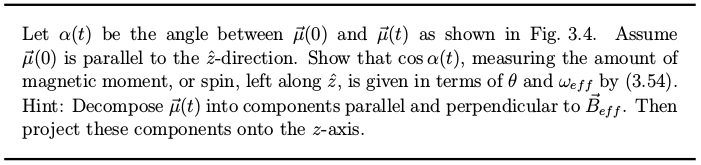
\includegraphics[width=0.8\textwidth,keepaspectratio]{prbl36}
    \label{fig:prbl36}
\end{figure}

\textit{Remember:}
\begin{itemize}
	\item The behaviour of the z-component of the magnetic moment is 
	shown here.
\end{itemize}

\begin{figure}[H]
        \centering
        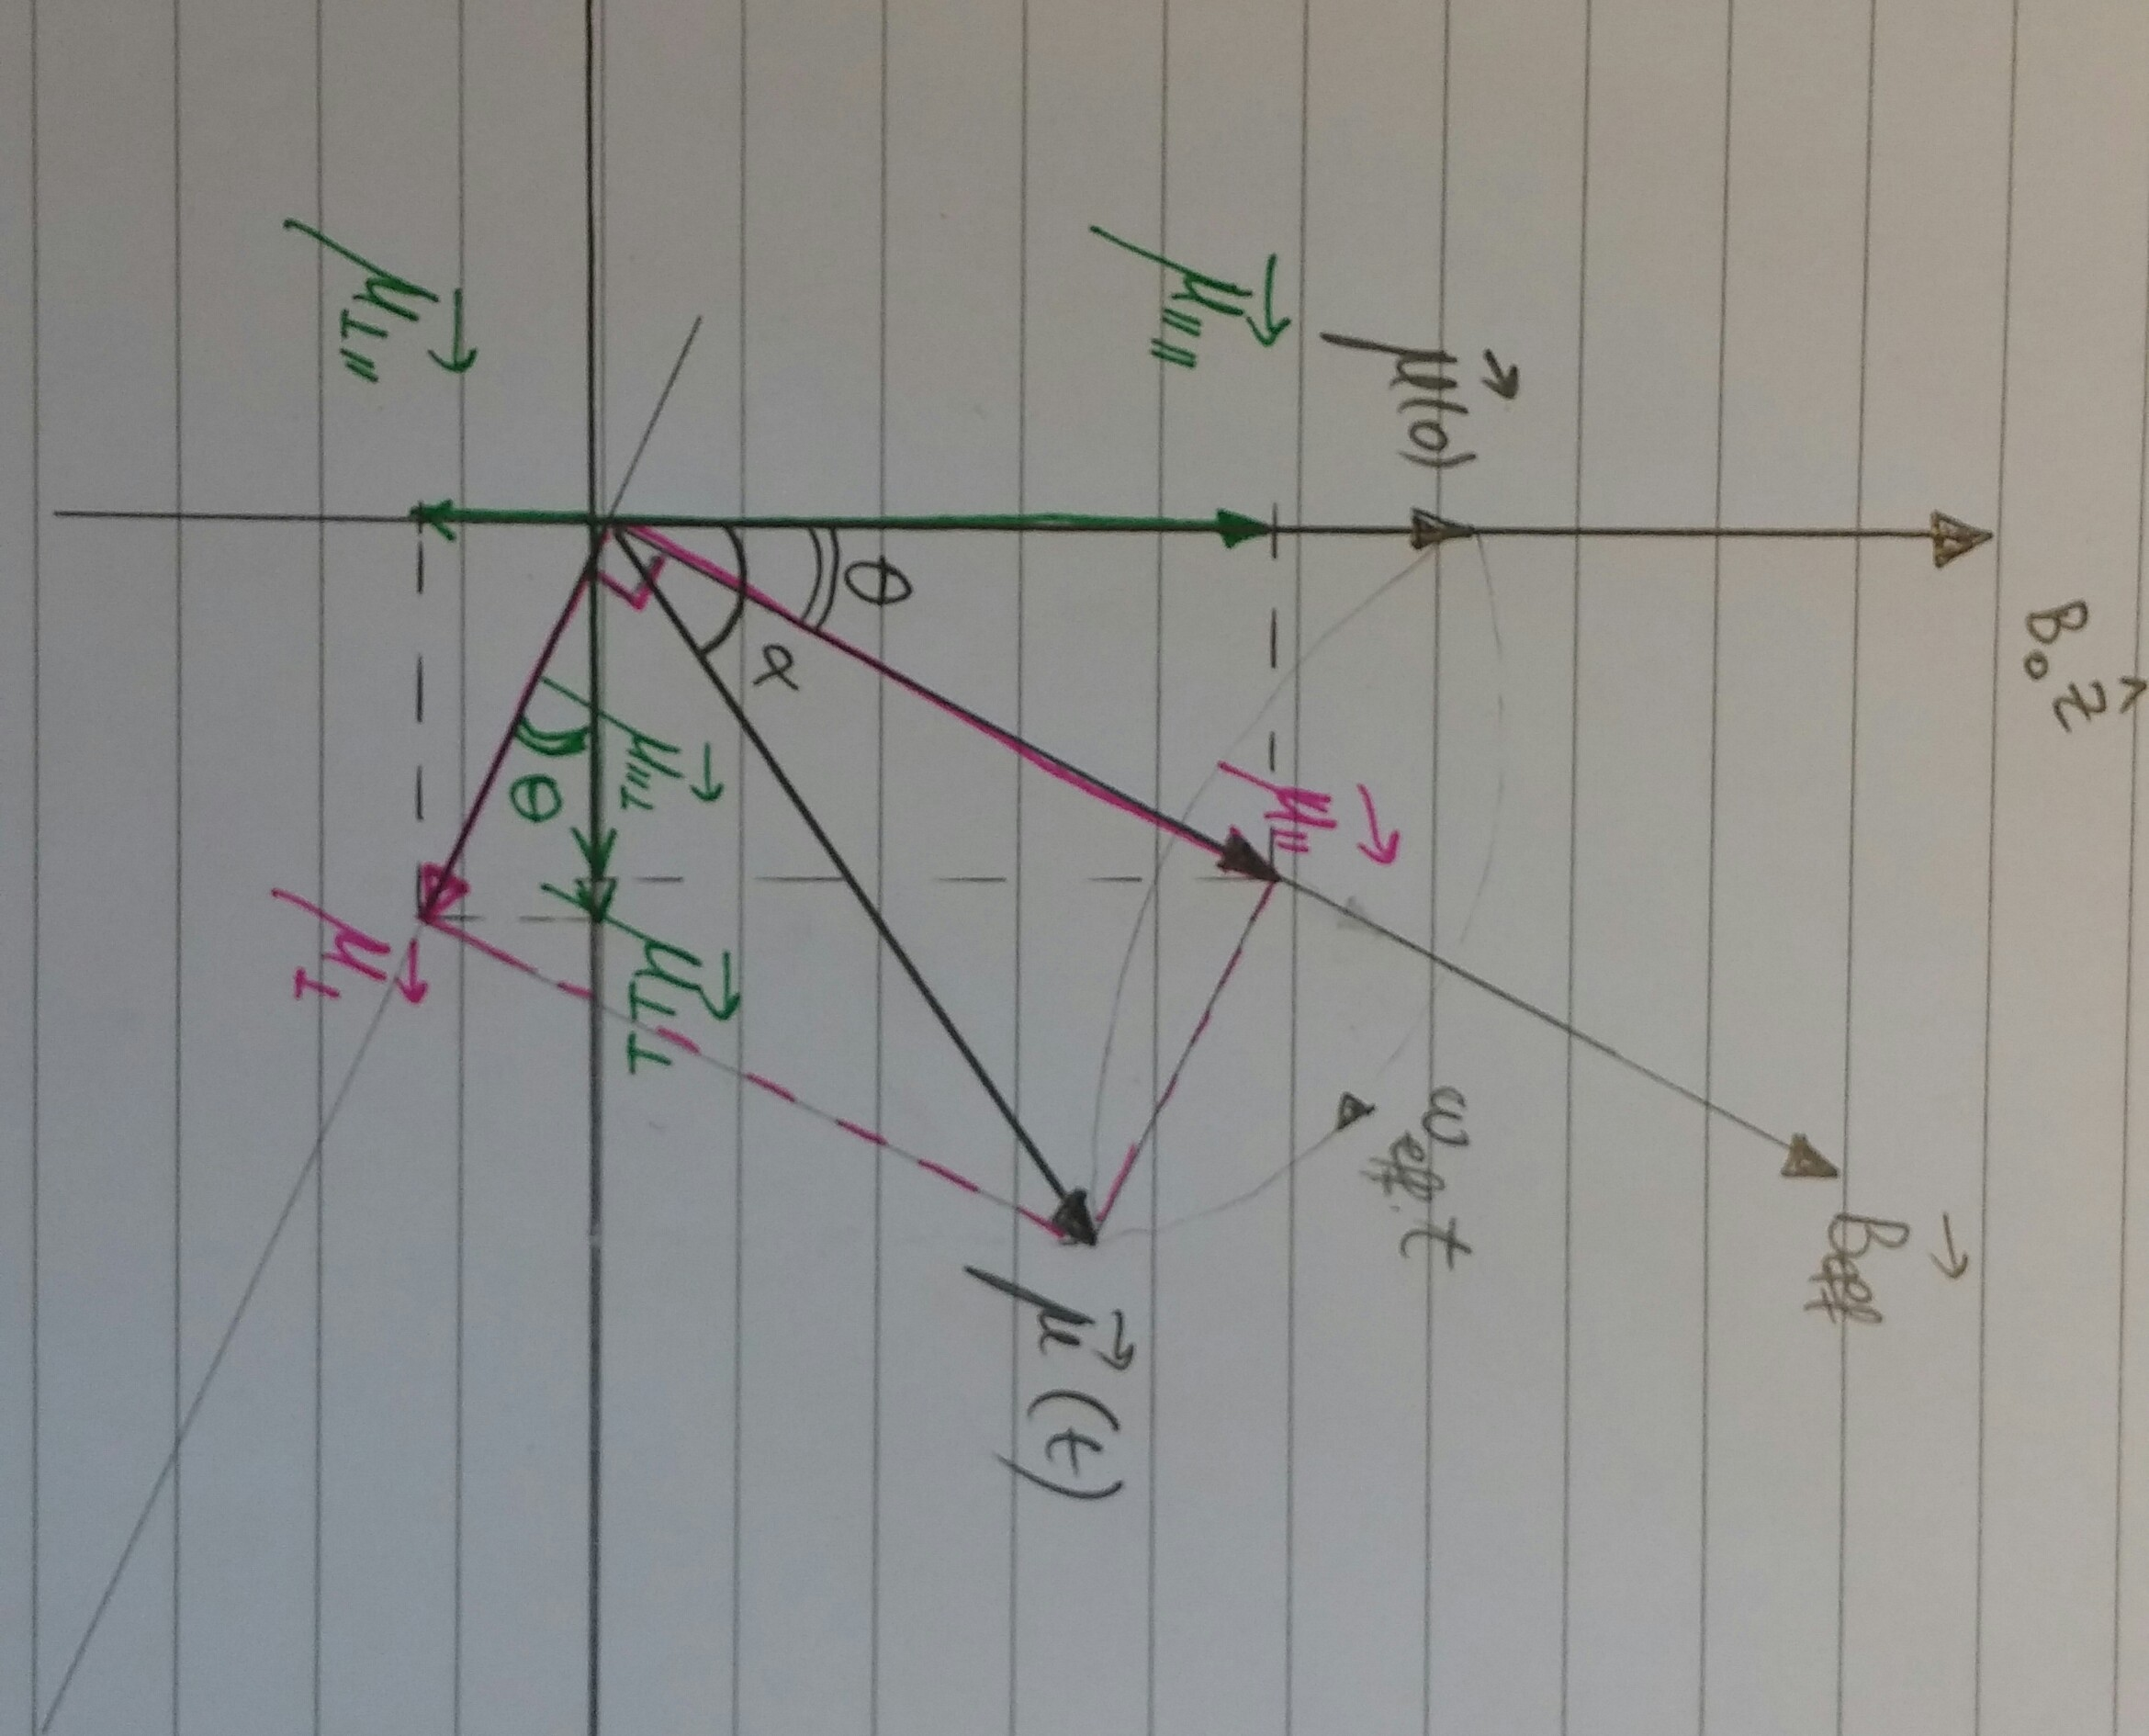
\includegraphics[angle=90,width=0.8\textwidth,keepaspectratio]{problem36}
        \label{fig:problem36}
\end{figure}

\textit{Proof.}

\begin{figure}[H]
        \centering
        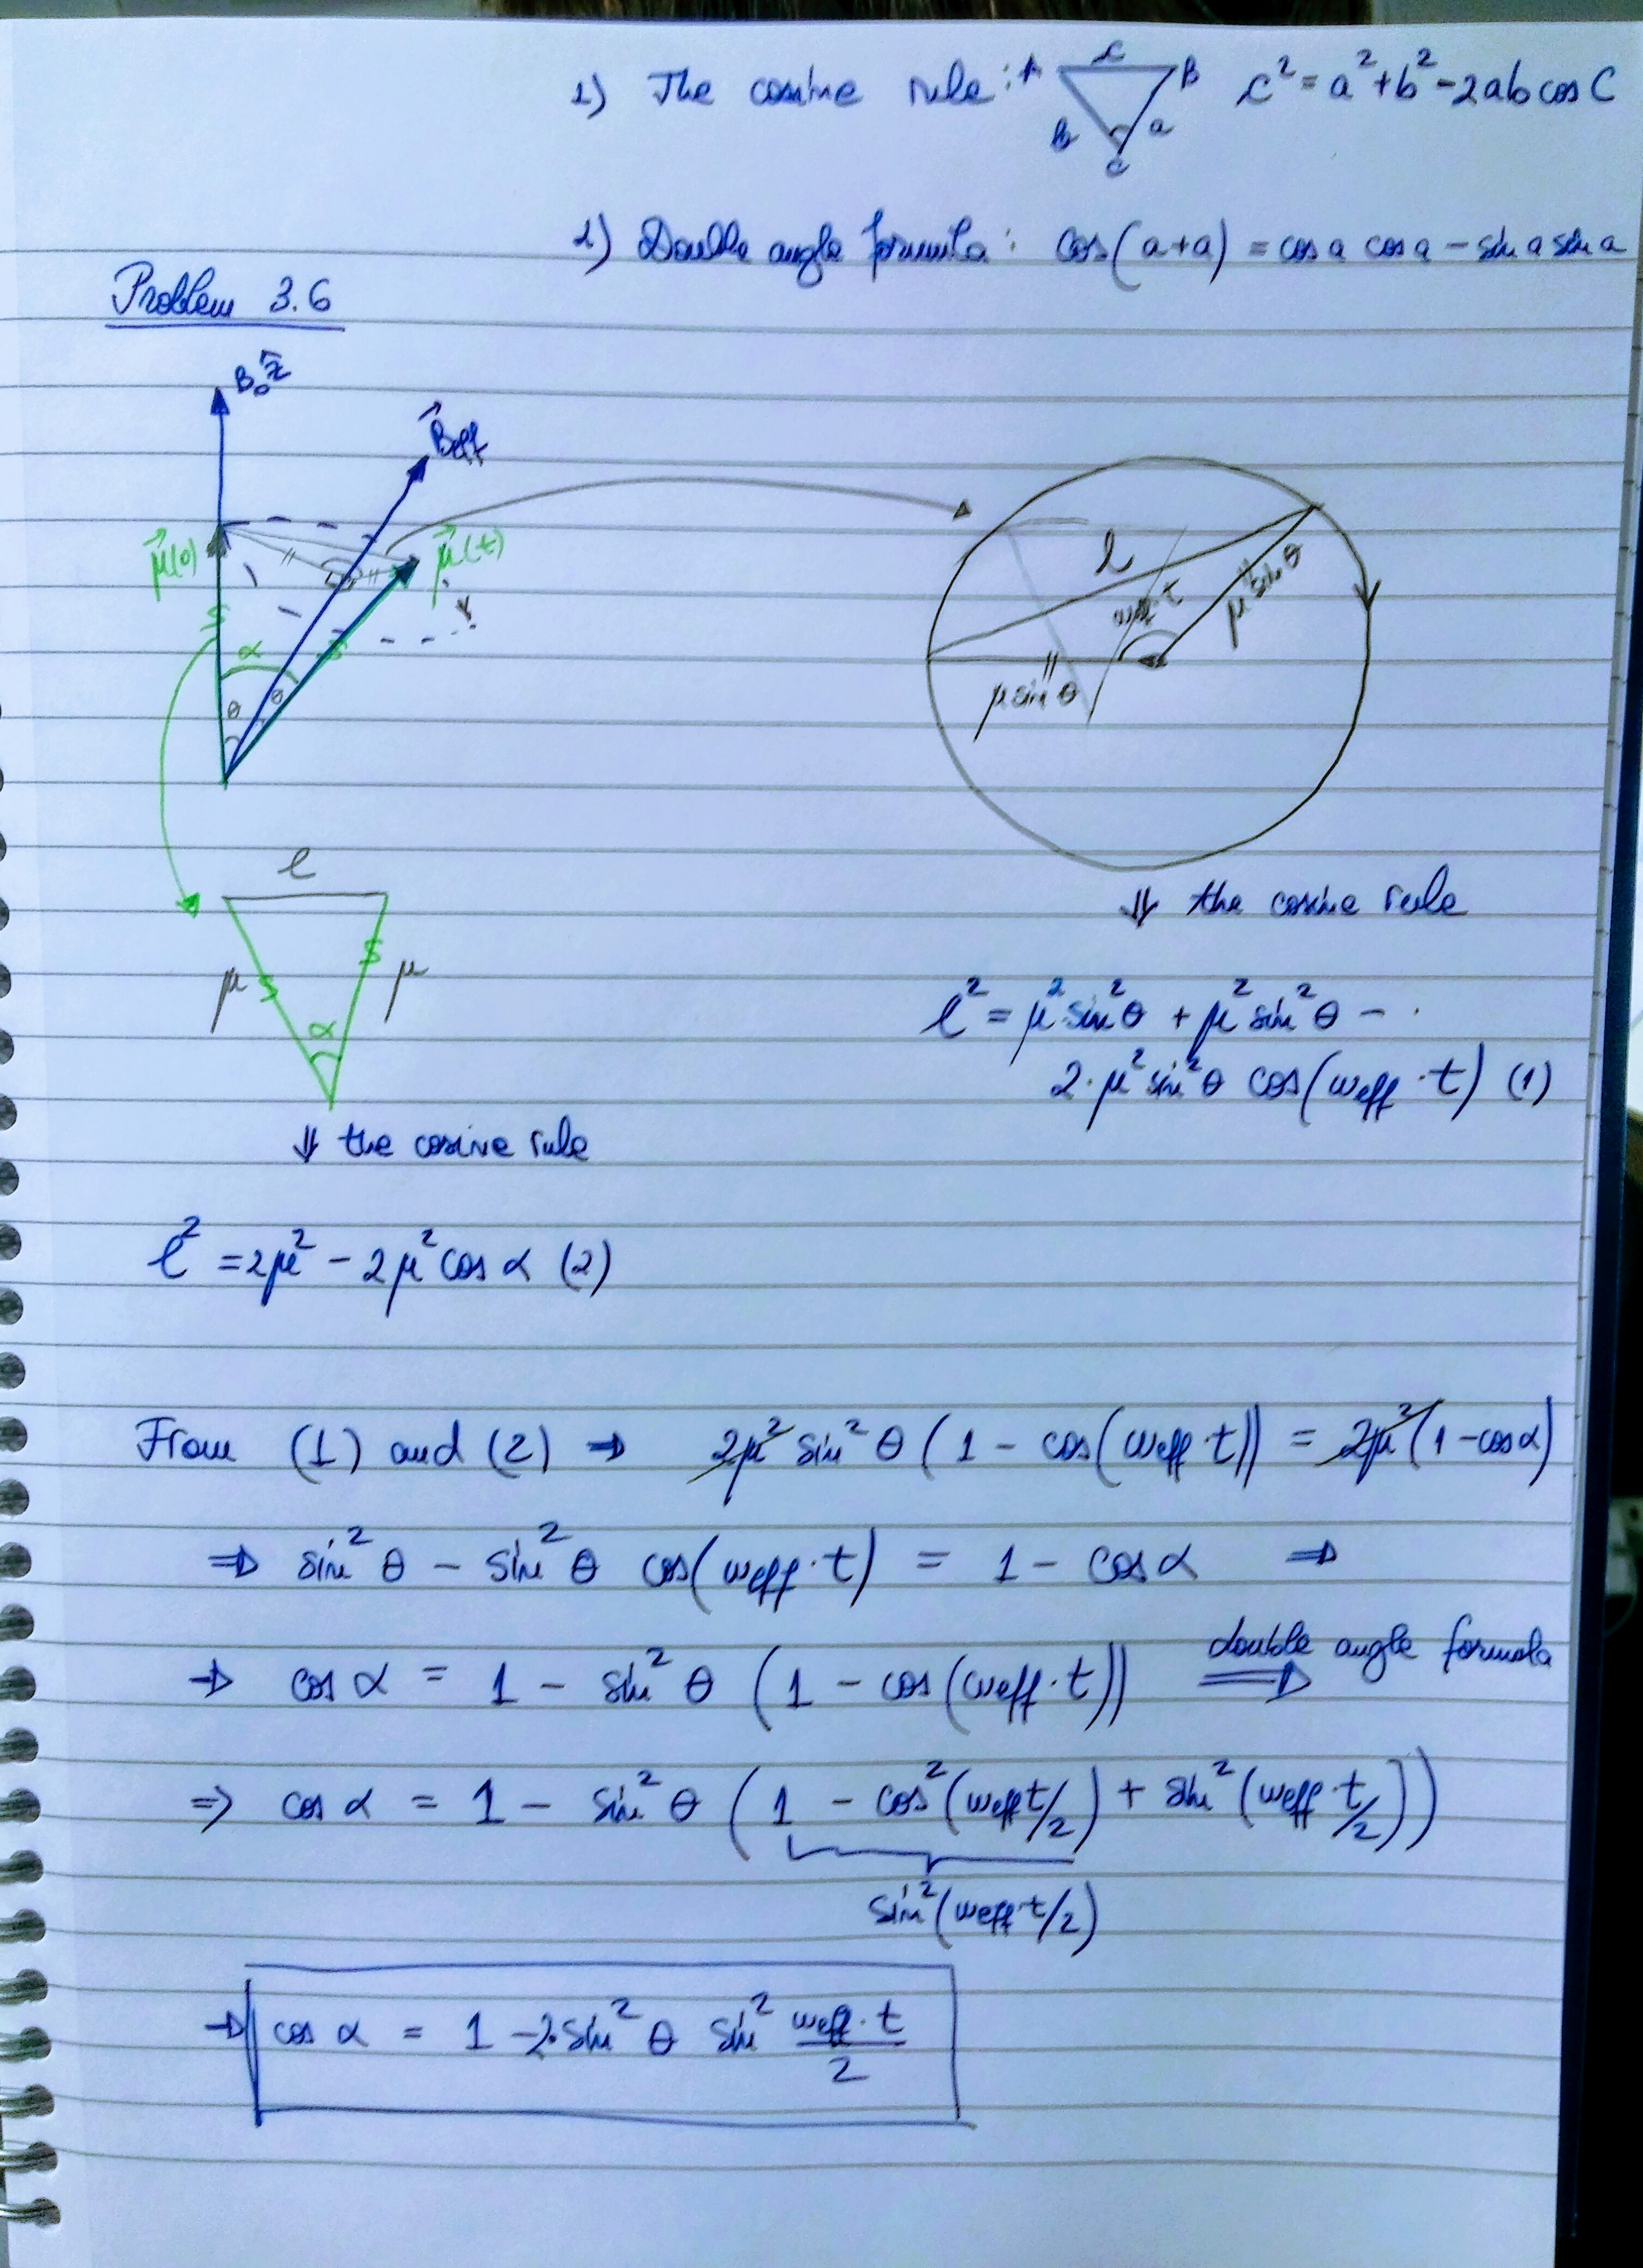
\includegraphics[width=0.8\textwidth,keepaspectratio]{problem36solution}
        \label{fig:problem36solution}
\end{figure}



\clearpage

%%%%%%%%%%%%%%%%%%%%%%%%%%%%%%
%% CHAPTER 4
%%%%%%%%%%%%%%%%%%%%%%%%%%%%%%
\newpage
\section{Magnetization, Relaxation, and the Bloch Equation}
\subsection{Summary}
\begin{enumerate}
    \item This chapter investigates the 

\end{enumerate}


\clearpage
%%%%%%%%%%%%%%%%%%%%%%%%%%%%%%
%% EXERCISES
\newpage
\subsection{Exercises}

%%%%%%%%%%%%%%%%%%%%%%%%%%%%%%
\Large{Problem 4.1}
\begin{figure}[H]
    \centering
    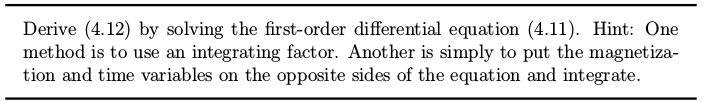
\includegraphics[width=0.8\textwidth,keepaspectratio]{prbl41}
    \label{fig:prbl41}
\end{figure}

\begin{figure}[H]
    \centering
    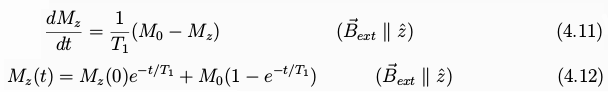
\includegraphics[width=0.8\textwidth,keepaspectratio]{form411412}
    \label{fig:form411412}
\end{figure}

\textit{Remember:}
\begin{itemize}
	\item After applying an RF pulse, the longitudinal magnetization 
	relaxes back to its equilibrium value ($M_0$), following an 
	exponential evolution from the initial value ($M_z(0)$).
\end{itemize}

\textit{Proof.}

\begin{flalign*}
    \frac{d M_z}{dt} &= \frac{1}{T_1} (M_0 - M_z) \\ 
    \frac{1}{M_0 - M_z} d M_z &= \frac{1}{T_1} dt \\
    \int_{M_z(0)}^{M_z(t)} \frac{1}{M_0 - M_z}d M_z &= \int_{t}^{0} \frac{1}{T_1} dt \\
    [ln(M_0 - M_z)]_{M_z(0)}^{M_z(t)} &= [\frac{t}{T_1}]_{t}^{0} \\
    ln \frac{M_0 - M_z(t)}{M_0 - M_z(0)} &= - \frac{t}{T_1} \\
    exp(ln \frac{M_0 - M_z(t)}{M_0 - M_z(0)}) &= exp (- \frac{t}{T_1}) \\
    \frac{M_0 - M_z(t)}{M_0 - M_z(0)} &= exp (- \frac{t}{T_1}) \\
    M_0 - M_z(t) &= M_0 \, e^{-t/T_1} - M_z(0) \, e^{-t/T_1} \\
    M_z(t) &= M_0 (1 - e^{-t/T_1}) + M_z(0) e^{-t/T_1}
\end{flalign*}

\clearpage
%%%%%%%%%%%%%%%%%%%%%%%%%%%%%%
\Large{Problem 4.2}
\begin{figure}[H]
    \centering
    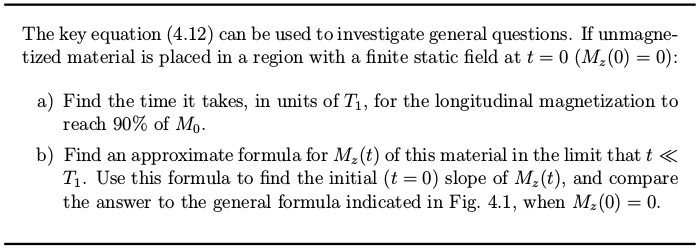
\includegraphics[width=0.8\textwidth,keepaspectratio]{prbl42}
    \label{fig:prbl42}
\end{figure}

\textit{Remember:}
\begin{itemize}
	\item Investigating general questions using $M_z(t) = M_z(0) e^{-t/T_1} + M_0 (1 - e^{-t/T_1})$
    \item \textit{Taylor Series}: \\
    $f(x) = f(a) + \frac{f'(a)}{1!} (x-a) + \frac{f''(a)}{2!} (x-a)^2 + \frac{f'''(a)}{3!} (x-a)^3 + ...$ \\
    \item \textit{Maclaurin Series} (is Taylor series for $a=0$): \\
    $f(x) = f(0) + \frac{f'(0)}{1!} x + \frac{f''(0)}{2!} x^2 + \frac{f'''(0)}{3!} x^3 + ...$ \\
    \item If $f(x) = e^{-t/T_1}$, then: $e^{-t/T_1} \approx 1 - \frac{t}{T_1} $ 
\end{itemize}

\textit{a) Proof.}\\
\textit{We know that:}\\
\begin{flalign*}
    M_z(t) &= 0.9 M_0 \\
    M_z(0) &= 0
\end{flalign*}

\textit{Therefore:}
\begin{flalign*}
    M_z(t) &= M_z(0) e^{-t/T_1} + M_0 (1 - e^{-t/T_1}) \\
    0.9 M_0 &= M_0 (1 - e^{-t/T_1}) \\
    e^{-t/T_1} &= 0.1 \\
    -t/T_1 &= ln(0.1) \\
    t &= 2.3 \, T_1
\end{flalign*}

\textit{b) Proof.}\\
\textit{We know that:}\\
\begin{flalign*}
    t \, << \, T_1
\end{flalign*}

\textit{Therefore:}
\begin{flalign*}
    M_z(t) &= M_z(0) e^{-t/T_1} + M_0 (1 - e^{-t/T_1}) \\
    [\frac{dM_z(t)}{dt}]_{t<<T_1} &= - [\frac{1}{T_1} M_z(0) e^{-t/T_1}]_{t<<T_1} + [\frac{1}{T_1} M_0 e^{-t/T_1}]_{t<<T_1} \\
    [\frac{dM_z(t)}{dt}]_{t<<T_1} &= - \frac{1}{T_1} M_z(0) + \frac{1}{T_1} M_0 \\
    [\frac{dM_z(t)}{dt}]_{t<<T_1} &= \frac{1}{T_1} ( M_0 - M_z(0) ) 
\end{flalign*}

\clearpage
%%%%%%%%%%%%%%%%%%%%%%%%%%%%%%
\Large{Problem 4.3}
\begin{figure}[H]
    \centering
    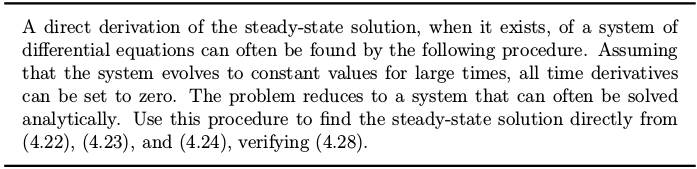
\includegraphics[width=0.8\textwidth,keepaspectratio]{prbl43}
    \label{fig:prbl43}
\end{figure}

\textit{Remember:}
\begin{itemize}
	\item Finding the steady-state solution.
\end{itemize}

\begin{figure}[H]
    \centering
    \includegraphics[width=0.8\textwidth,keepaspectratio]{form422423424}
    \label{fig:form422423424}
\end{figure}
\begin{figure}[H]
    \centering
    \includegraphics[width=0.8\textwidth,keepaspectratio]{form428}
    \label{fig:form428}
\end{figure}

\textit{Proof.}
\begin{flalign*}
    \frac{M_0 - M_z}{T_1} &= 0 \\
    \omega_0 M_y - \frac{M_x}{T_2} &= 0 \\
    - \omega_0 M_x - \frac{M_y}{T_2} &= 0 \\
    & \Rightarrow \\
    M_z &= M_0 \\
    M_x &= \omega_0 T_2 M_y \\
    M_y &= \omega_0 T_2 M_x \\
    & \Rightarrow \\
    M_z &= M_0 \\
    M_x &= \omega_0 T_2 M_y \\
    M_y &= \omega_0 T_2 M_x \\
    (M_x + M_y) &= \omega_0 T_2 (M_x + M_y) \rightarrow \omega_0 T_2 = 1\\
    & \Rightarrow \\
\end{flalign*}
\begin{flalign*}
    M_z &= M_0 \\
    M_x &= M_y \\
    \omega_0 M_x - \frac{M_x}{T_2} &= 0 \rightarrow M_x(\omega_0 - \frac{1}{T_2}) = 0 \rightarrow M_x = 0\\
    & \Rightarrow \\
    M_x(\infty) &= M_y(\infty) = 0 \\
    M_z(\infty) &= M_0 
\end{flalign*}

\textit{Or:}
\begin{flalign*}
    \lim_{t \rightarrow \infty} M_x(t) &= \lim_{t \rightarrow \infty} e^{-t/T_2} (M_x(0) cos \omega_0 t + M_y(0) sin \omega_0 t) = 0 \\
    \lim_{t \rightarrow \infty} M_y(t) &= \lim_{t \rightarrow \infty} e^{-t/T_2} (M_y(0) cos \omega_0 t - M_x(0) sin \omega_0 t) = 0\\
    \lim_{t \rightarrow \infty} M_z(t) &= \lim_{t \rightarrow \infty} M_z(0) e^{-t/T_1} + M_0 (1 - e^{-t/T_1}) = M_0 \\
    & \Rightarrow \\
    M_x(\infty) &= M_y(\infty) = 0 \\
    M_z(\infty) &= M_0 
\end{flalign*}


\clearpage
%%%%%%%%%%%%%%%%%%%%%%%%%%%%%%
\Large{Problem 4.4}
\begin{figure}[H]
    \centering
    \includegraphics[width=0.8\textwidth,keepaspectratio]{prbl44}
    \label{fig:prbl44}
\end{figure}

\textit{Remember:}
\begin{itemize}
	\item The complex representation solutions.
\end{itemize}


\textit{a) Proof.}
%   \frac{d M_{+}}{dt} &= (-i \omega_0 - \frac{1}{T_2}) M_+ \\
%    \frac{d M_{+}}{dt} &= (-i \omega_0 - \frac{1}{T_2}) (M_x + i M_y) \\
%    \frac{d M_{+}}{dt} &= -i \omega_0 M_x + \omega_0 M_y - \frac{1}{T_2} M_x - \frac{i}{T_2} M_y \\
%    \frac{d M_{+}}{dt} &= i M_y(-i \omega_0 - \frac{1}{T_2}) + M_x (-\frac{1}{T_2} - i \omega_0) \\
%    \frac{d M_{+}}{dt} &= (-i \omega_0 - \frac{1}{T_2}) (M_x + i M_y) \\
% 
\begin{flalign*}
    \frac{d M_{+}}{dt} &= (-i \omega_0 - \frac{1}{T_2}) M_+ \\
    \frac{1}{M_{+}} d M_{+} &= (-i \omega_0 - \frac{1}{T_2}) dt \\
    \int_{M_{+}(0)}^{M_{+}(t)} \frac{1}{M_{+}} d M_{+} &= \int_{0}^{t} (-i \omega_0 - \frac{1}{T_2}) dt \\
    ln \frac{M_{+}(t)}{M_{+}(0)} &= t(-i \omega_0 - \frac{1}{T_2}) \\
    \frac{M_{+}(t)}{M_{+}(0)} &= e^{-i \omega_0 t - \frac{t}{T_2}} \\
    M_{+}(t) &= M_{+}(0) e^{-i \omega_0 t - \frac{t}{T_2}} \\
\end{flalign*}


\clearpage
%%%%%%%%%%%%%%%%%%%%%%%%%%%%%%
\Large{Problem 4.5}
\begin{figure}[H]
    \centering
    \includegraphics[width=0.8\textwidth,keepaspectratio]{prbl45}
    \label{fig:prbl45}
\end{figure}

\textit{Remember:}
\begin{itemize}
	\item The Bloch equations magnetization components in the primed basis.
\end{itemize}


\begin{figure}[H]
    \centering
    \includegraphics[width=0.8\textwidth,keepaspectratio]{form421}
    \label{fig:form421}
\end{figure}

\begin{figure}[H]
    \centering
    \includegraphics[width=0.8\textwidth,keepaspectratio]{form437438439}
    \label{fig:form437438439}
\end{figure}

\textit{Proof.}
\begin{flalign*}
    (\frac{d \vec{M}}{dt})' &= \gamma \vec{M}' \times \vec{B}_{eff} + \frac{1}{T_1} 
    (M_0 - M_z) \hat{z} - \frac{1}{T_2} (M_{x'} \hat{x}' + M_{y'} 
    \hat{y}') \\
    &= \gamma \vec{M}' \times [(B_0 - \omega / \gamma) \hat{z} + B_1 
    \hat{x}'] + \frac{1}{T_1} 
    (M_0 - M_z) \hat{z} - \frac{1}{T_2} (M_{x'} \hat{x}' + M_{y'} 
    \hat{y}') \\
    &= \gamma(B_0 - \omega / \gamma) (- M_{x'} \hat{y}' + M_{y'} 
    \hat{x}') + \gamma B_1 (- M_{y'} \hat{z} + M_{z} \hat{y}') \\
    &+ \frac{1}{T_1} 
    (M_0 - M_z) \hat{z} - \frac{1}{T_2} (M_{x'} \hat{x}' + M_{y'} 
    \hat{y}') \Rightarrow \\ 
    (\frac{d M_z}{dt})' &= -\omega_1 M_{y'} + \frac{M_0 - 
    M_z}{T_1} \\
    (\frac{d M_x}{dt})' &= (\omega_0 - \omega) M_{y'} - 
    \frac{M_{x'}}{T_2} \\
    (\frac{d M_y}{dt})' &= -(\omega_0 - \omega) M_{x'} + \omega_1 M_z - 
    \frac{M_{y'}}{T_2} \\
    & \Rightarrow \\
    (\frac{d M_z}{dt})' &= -\omega_1 M_{y'} + \frac{M_0 - 
    M_z}{T_1} \\
    (\frac{d M_x}{dt})' &= \Delta \omega M_{y'} - 
    \frac{M_{x'}}{T_2} \\
    (\frac{d M_y}{dt})' &= - \Delta \omega M_{x'} + \omega_1 M_z - 
    \frac{M_{y'}}{T_2} \\
\end{flalign*}

\clearpage
%%%%%%%%%%%%%%%%%%%%%%%%%%%%%%
\Large{Problem 4.6}
\begin{figure}[H]
    \centering
    \includegraphics[width=0.8\textwidth,keepaspectratio]{prbl46}
    \label{fig:prbl46}
\end{figure}

\textit{Remember:}
\begin{itemize}
	\item    
\end{itemize}


\textit{Proof.}



\clearpage

%%%%%%%%%%%%%%%%%%%%%%%%%%%%%%
%% CHAPTER 11
%%%%%%%%%%%%%%%%%%%%%%%%%%%%%%
\newpage
\section{The Continuous and Discrete Fourier Transforms}
\label{ch:11}

\textit{Summary}
\begin{itemize}
    \item This chapter is focused on the continuous and discrete Fourier Transforms relevant to MR imaging.

    \item In the absence of relaxation effects, $s(\vec{k})$ and $\rho(\vec{r})$ are \textbf{Fourier transform pairs}.

    \item The reconstructed image, $\hat{\rho}(\vec{r})$, represents an \textbf{estimate} of the \textbf{effective spin density} due to various \textbf{numerical approximations} that take place during the MR imaging process (from \textbf{discretised} and \textbf{truncated} signal sampling).    
\end{itemize}

\begin{figure}[H]
    \centering
    \includegraphics[width=.6\textwidth,keepaspectratio]{FourierJeanBaptiste}
    \caption{Jean-Baptiste Joseph Fourier \courtesywiki}
    \label{fig:FourierJeanBaptiste}
\end{figure}


\clearpage
%%
\subsection{The Continuous Fourier Transform}

\begin{itemize}

    \item The \textbf{Fourier transform is a functional}, mapping a function to another function. \\ \\
    Let: \\
    $h$ be a function of x-space (or time space) and \\
    $H$ be a function of k-space (or frequency space) then: \\
    \begin{flalign*}
        \mathfrak{F}      & : (h) \rightarrow (H) \\
        \mathfrak{F}^{-1} & : (H) \rightarrow (h)   \\
        \mathfrak{F} \circ \mathfrak{F}^{-1} & = \text{identity}
    \end{flalign*}

    In MRI, the \textbf{Fourier transform maps a function} from \textbf{position space (x-space)} to its \textbf{'conjugate' space (k-space)}, and back, through the inverse Fourier transform.

    \item Fourier Transform Pairs in MRI: $\rho(\vec{r}) \xLeftrightarrow{\mathfrak{F}} s(\vec{k})$, where \\
    $\rho(\vec{r})$ = \textbf{spin density in x-space (position space)} and \\
    $s(\vec{k})$ = \textbf{signal in k-space (spatial frequency space)}

    \item Knowing the \textbf{signal equation }: \\
    \begin{flalign*}
        s(\vec{k}) = \int_{- \infty}^{+ \infty} d\vec{r} \ \rho(\vec{r}) e^{-i 2 \pi \vec{k} \cdot \vec{r}}
    \end{flalign*}
    the \textbf{Fourier transform pairs} are shown for the general case: \\
    \begin{flalign*}
        H(\vec{k}) \equiv \mathfrak{F}(h(\vec{r})) & = \int_{- \infty}^{+ \infty} d\vec{r} \ h(\vec{r}) e^{-i 2 \pi \vec{k} \vec{r}} \\ 
        h(\vec{r}) \equiv \mathfrak{F}^{-1}(H(\vec{k})) & = \int_{- \infty}^{+ \infty} d\vec{k} \ H(\vec{k}) e^{+i 2 \pi \vec{k} \vec{r}} 
    \end{flalign*}
    and for \textbf{Dirac delta functions}, knowing from (Book 9.24) that $\delta(\vec{r}) = \int_{- \infty}^{+ \infty} d\vec{k} \ e^{i 2 \pi \vec{k} \cdot \vec{r}}$, we have:
    \begin{flalign*}
        \delta(\vec{k} - \vec{k}_0) & = \int_{- \infty}^{+ \infty} d\vec{r} \ e^{-i 2 \pi (\vec{k}-\vec{k}_0) \cdot \vec{r}} \\ 
        \delta(\vec{r} - \vec{r}_0) & = \int_{- \infty}^{+ \infty} d\vec{k} \ e^{+i 2 \pi \vec{k} \cdot (\vec{x}-\vec{x}_0) }
    \end{flalign*}
    
    \textcolor{gray}{\textbf{Sidenote}: $\delta(\vec{r}) \equiv \mathfrak{F}^{-1}(G(\vec{k})) = \int_{- \infty}^{+ \infty} d\vec{k} \ G(\vec{k}) \  e^{i 2 \pi \vec{k} \cdot \vec{r}} \Rightarrow G(\vec{k}) = 1$. This is very interesting as we have seen in Book Chapter 9.3.1, that $\delta(x) = \lim_{K\to\infty} 2K \ sinc(2 \pi K x)$ (see Figure~\ref{fig:figeq928}), which shows that, at the limit, the Dirac delta function encompasses all possible frequencies. Therefore, its Fourier transform will be a straight line.}
    
    \item The identity property ($\mathfrak{F} \circ \mathfrak{F}^{-1} = \text{identity}$) can be derived like this: \\
    \begin{flalign*}
        h(x) & = \int_{- \infty}^{+ \infty} dk \ H(k) e^{+i 2 \pi k x} \\
             & = \int_{- \infty}^{+ \infty} dk \ \int_{- \infty}^{+ \infty} dx' \ h(x') e^{-i 2 \pi k x'} \ \ e^{+i 2 \pi k x} \\
             & = \int_{- \infty}^{+ \infty} dx' \ h(x') \int_{- \infty}^{+ \infty} dk \ e^{+i 2 \pi k (x-x')} \\
             & = \int_{- \infty}^{+ \infty} dx' \ h(x') \delta(x-x') \text{ (See Book 9.27)}\\
             & = h(x)
    \end{flalign*}

    \item A continuous signal $s(k)$, known for all $k$, can be used to retrieve the \textbf{spin density} (Book 11.7): \\
    \begin{flalign*}
        \rho(\vec{r}) = \int_{- \infty}^{+ \infty} d\vec{k} \ s(\vec{k}) e^{+i 2 \pi \vec{k} \cdot \vec{r}}
    \end{flalign*}
    In fact, the signal is not known for all $k$, but it is an approximation of the continuous form. \\
    The actual signal is finitely sampled, it is called $s_m(k)$ (measured signal) and it yields the reconstructed image $\hat{\rho(x)}$ through a continuous inverse Fourier transform:
    \begin{flalign*}
        \hat{\rho}(\vec{r}) = \int_{- \infty}^{+ \infty} d\vec{k} \ s_m(\vec{k}) e^{+i 2 \pi \vec{k} \cdot \vec{r}}
    \end{flalign*}

    \item The differences between $\rho(\vec{r})$ and $\hat{\rho}(\vec{r})$ are very important in understanding imaging artifacts.
\end{itemize}

\begin{figure}[H]
    \centering
    \includegraphics[width=.7\textwidth,keepaspectratio]{figeq928}
    \caption{When the $sinc$ argument increases ($K$ increases), the $sinc$ function becomes narrower and narrower. The term outside of the $sinc$ function increases its amplitude. Therefore, the larger the $K$, the closer the $I(x,K) = 2K sinc(2\pi \ K x)$ function gets to the Dirac delta.}
    \label{fig:figeq928}
\end{figure}




\clearpage
%%
\subsection{Continuous Fourier Transform Properties and Phase Imaging}
Properties of the continuous Fourier transform are introduced here. It is again mentioned the fact that differences between $\hat{\rho}(x)$ and $\rho(x)$ are generally called artifacts.

%
\subsubsection{Complexity of the Reconstructed Image}

\begin{itemize}
    
    \item Complexity of the reconstructed image refers to the fact that $\hat{\rho}(x)$ can be a complex-valued quantity unlike its ideal continuous version $\rho(x)$. This difference can be due to a switch between the real and imaginary RF receiver channels or an incorrect demodulation that can lead to the presence of a \textbf{global (constant) phase shift $\phi_0$ in the signal}. 

    \item This signal can be written as:
    \begin{flalign*}
        \widetilde{s}(k) = e^{i \phi_0} s(k)
    \end{flalign*}
    where $s(k)$ is the real/true signal.\\
    
    The reconstructed image will then be:
    \begin{flalign*}
        \hat{\rho}(x) & = \int_{- \infty}^{+ \infty} dk \ \widetilde{s}(k) e^{+i 2 \pi kx} \\
        & = e^{i \phi_0} \ \int_{- \infty}^{+ \infty} dk \ s(k) e^{+i 2 \pi kx} \\
        & = e^{i \phi_0} \rho(x)
    \end{flalign*}

    \item This is the reason why, in practice, magnitude images are used in order to get  $\rho(x)$ independent of $\phi_0$. The magnitude image is calculated as:
    \begin{flalign*}
        \hat{\rho}(x) & = e^{i \phi_0} \rho(x) \\
                      & = cos(\phi_0) \rho(x) + i \ sin(\phi_0) \rho(x) \\
        \lvert \hat{\rho}(x) \rvert & = \sqrt{\rho(x)^2 \ (cos^2(\phi_0) + sin^2(\phi_0))} = \lvert \rho(x) \rvert
    \end{flalign*}
    
\end{itemize}


%
\subsubsection{The Shift Theorem}

\begin{itemize}
    \item The Fourier Transform Shift Theorem shows that a shift in one space will translate into a global constant phase in its Fourier transform. In terms of MRI, the Fourier transform shift theorem is an important concept because it explains what happens to the reconstructed image when there is \textbf{a) a shift in the echo relative to its expected location} (see Figure~\ref{fig:fig112}) or due to \textbf{b) incorrect demodulation} (demodulation at the wrong frequency).

    \item Cases:  
    \begin{enumerate}
        \item \textbf{A linear shift of the k-space origin} will create an additional phase in the reconstructed image $\hat{\rho}(x)$. A magnitude image will faithfully reconstruct $\rho(x)$. \\
        
        The shift in k-space moves by $k_0$ from where it was expected. This means that $s_m(k) \rightarrow s_m(k-k_0)$. Taking the inverse Fourier transform of the shifted measured signal shows that the reconstruction will have an additional global phase in addition to the expected reconstruction for a non-shifted k-space.
        \begin{flalign*}
            \hat{\rho}(x) & = \mathfrak{F}^{-1}(s_m(k-k_0)) \\
            & = \int_{- \infty}^{+ \infty} dk \ s_m(k-k_0) e^{i 2 \pi k x} \\
            \text{Change of variable: } k' & = k - k_0 \\
            & = e^{i 2 \pi k_0 x} \ \int_{- \infty}^{+ \infty} dk' \ s_m(k') e^{i 2 \pi k' x} \\
            & = e^{i 2 \pi k_0 x} \ \hat{\rho}_{expected}(x)
        \end{flalign*}

        \item \textbf{A linear phase shift in the k-space data} ($s_m(k) \rightarrow s_m(k) e^{-i 2 \pi k x_0}$) will lead to a spatial shift (of $x_0$) in the reconstructed image.
        \begin{flalign*}
            \rho(x') & = \int_{- \infty}^{+ \infty} dk \ s(k) e^{+ i 2 \pi k x'} \\
            \text{Change of variable: } x' & = x - x_0 \Rightarrow \\
            \rho(x - x_0) & = \int_{- \infty}^{+ \infty} dk \ s(k) e^{+ i 2 \pi k (x-x_0)} \\
            & =\int_{- \infty}^{+ \infty} dk \ s(k)  e^{- i 2 \pi k x_0} \  e^{+ i 2 \pi k x} \\
            & = \mathfrak{F}^{-1}(s(k) \ e^{- i 2 \pi k x_0} )  
        \end{flalign*}
        
    \end{enumerate}

\end{itemize}

\begin{figure}[H]
    \centering
    \includegraphics[width=.7\textwidth,keepaspectratio]{fig112}
    \caption{Example of a read gradient structure leading to a shift of the echo in the sampling window. The area under the gradient between $t_1$ and $t_2$ is $A$ and the area under the read gradient itself is $2B$. The echo is shifted from $TE$ to $TE' < TE$ if $A$ is chosen to be less than $B$. This results in a shift of $k_0 < 0$ in the read direction k-space variable. \newline \courtesy}
    \label{fig:fig112}
\end{figure}

%
\subsubsection{Phase Imaging and Phase Aliasing}

\begin{itemize}
    \item Phase imaging is a technique used in MRI where images of the accumulated phase are constructed instead of the classic anatomical or functional ones. Phase images are calculated with the inverse tangent as presented here:
    \begin{flalign*}
        \phi(x,y) \equiv Arg \ \hat{\rho}(x,y) = tan^{-1} \Bigg( \frac{Im \  \hat{\rho}(x,y)}{Re \ \hat{\rho}(x,y)} \Bigg)
    \end{flalign*}
    One particular usefulness is to see whether the expected gradient echo is uncentered. 

    \item Phase Imaging artifact (see Figure~\ref{fig:fig113}):
    \begin{itemize}
        \item \textit{Zebra stripes} are a phase imaging artifact that can be caused by an \textbf{asymmetry in the echo position}. Because of the inverse tangent’s periodicity, spins with phase values differing by multiples of $2\pi$ will have the same intensity and this will cause the aforementioned artifact.

        \item How? 
        The centre of the sampling window is expected to be at $k = 0$, for which the readout gradient phase for all spins is $0$. When this is no longer true, and a certain shift of $k_0$ has happened in the way data was sampled, the measured signal $s_m(k)$ is no longer the true (expected) $s(k)$. Instead, $s_m(k) = s(k-k_0)$.

        \item Applying the shift theorem here yields a reconstructed image in x-space that will also have an additional phase $\Delta \phi(x) = 2\pi k_0 x$.
    \end{itemize}

    \item Besides the gradient echo asymmetry, local field inhomogeneities also cause changes in the phase images.

\end{itemize}

\begin{figure}[H]
    \centering
    \includegraphics[width=.7\textwidth,keepaspectratio]{fig113}
    \caption{(a) A 2D gradient echo magnitude image of the head. (b) The corresponding phase image of the head when the echo is centered in the read data acquisition window. (c) A phase image taken from the same data that produced (b) except that the echo is shifted 'one sample point' away from the center of the sampling window. (d) A phase image where the echo is shifted five points away from the center of the sampling window. The restricted variation of the phase from $−\pi$ to $\pi$ creates the banding referred to as the 'zebra stripe' artifact. The phase shift occurs along the read (vertical) direction, and the bands are perpendicular to this direction. This is an example of how knowledge of the theory behind an artifact gives information about the sequence acquisition. \newline \courtesy}
    \label{fig:fig113}
\end{figure}

%
\subsubsection{The Duality Theorem}

\begin{itemize}
    \item The Duality Theorem states that if $h(x)$ and $H(k)$ are Fourier transform pairs, then $H(-x)$ and $h(k)$ are also Fourier transform pairs.

    \item Why this is important? 
    \begin{itemize}
        \item Knowing one pair of Fourier transforms will lead to knowing a different pair without any other calculations.
        
        \item Explanation from \href{https://ocw.mit.edu/resources/res-6-007-signals-and-systems-spring-2011/lecture-notes/MITRES_6_007S11_lec09.pdf}{here}: \\
        
            \begin{mdframed}[backgroundcolor=lightgray!20] 
                Duality between the time and frequency domains is another important
                property of Fourier transforms.
                This property relates to the fact that the analysis equation and synthesis equation look almost identical except for a factor
                of $1/2\pi$ and the difference of a minus sign in the exponential in the integral. 
                As a consequence, if we know the Fourier transform of a specified time function, then we also know the Fourier transform of a signal whose functional form is the same as the form of this Fourier transform. 
                Said another way, \textit{the Fourier
                transform of the Fourier transform is proportional to the original signal reversed
                in time}. 
                One consequence of this is that whenever we evaluate one
                transform pair we have another one for free.
                As another consequence, if we
                have an effective and efficient algorithm or procedure for implementing or
                calculating the Fourier transform of a signal, then exactly the same procedure
                with only minor modification can be used to implement the inverse Fourier
                transform. This is, in fact, very heavily exploited in discrete-time signal analysis
                and processing, where explicit computation of the Fourier transform and
                its inverse play an important role.
                [Quotation courtesy of \href{https://ocw.mit.edu/resources/res-6-007-signals-and-systems-spring-2011/lecture-notes/MITRES_6_007S11_lec09.pdf}{MIT}]
            \end{mdframed}
    
    \end{itemize}
    
    \item Deriving the duality theorem \label{proof:duality} (if $h(x) \xLeftrightarrow{\mathfrak{F}} H(k)$, then $H(-x) \xLeftrightarrow{\mathfrak{F}} h(k)$):
    % H(k) \equiv \mathfrak{F}(h(x)) & = \int_{- \infty}^{+ \infty} dx \ h(x) e^{-i 2 \pi kx} \\ 
    \begin{flalign*}
        \text{1) Starting from: } h(x) & = \int_{- \infty}^{+ \infty} dk \ H(k) e^{+i 2 \pi kx} \\
        \text{Change of variable } k & \rightarrow -k \\
        h(x) & = \int_{- \infty}^{+ \infty} dk \ H(-k) e^{-i 2 \pi kx} = \mathfrak{F}(H(-k)) \\
        \text{Change of variable } k & \rightarrow x \\
        h(k) & = \int_{- \infty}^{+ \infty} dx \ H(-x) e^{-i 2 \pi kx} = \mathfrak{F}(H(-x)) 
    \end{flalign*}
    
    \begin{flalign*}
        \text{2) Starting from: } H(k) & = \int_{- \infty}^{+ \infty} dx \ h(x) e^{-i 2 \pi kx} \\ 
        \text{Change of variable } k & \rightarrow -k \\
        H(-k) & = \int_{- \infty}^{+ \infty} dx \ h(x) e^{+i 2 \pi kx} = \mathfrak{F}^{-1}(h(x))\\ 
        \text{Change of variable } k & \rightarrow x \\
        H(-x) & = \int_{- \infty}^{+ \infty} dk \ h(k) e^{+i 2 \pi kx} = \mathfrak{F}^{-1}(h(k))
    \end{flalign*}
    
    \item Duality theorem for shifted Delta function ($\delta(x) \rightarrow \delta(x − x_0)$):
    \begin{flalign*}
        h(x) = \delta(x-x_0) & \xLeftrightarrow{\mathfrak{F}} H(k) = e^{−i2 \pi k x_0} \\
        & \text{and}  \\
        H(-x) = e^{+i2 \pi k x_0} & \xLeftrightarrow{\mathfrak{F}} h(k) = \delta(k-k_0)
    \end{flalign*}
    The shifted Delta function gives rise to a periodic transform with period $1/x_0$ as seen in Figure~\ref{fig:fig1124a}.
    
    \item A classic Fourier transform pair for MRI can be seen in both Figure~\ref{fig:fig1124b} and Figure~\ref{fig:fig1124bBook}, for the $rect(\frac{x}{W}) \xLeftrightarrow{\mathfrak{F}} W \ sinc(\pi Wk)$.

\end{itemize}

\begin{figure}[H]
    \centering
    \includegraphics[width=.9\textwidth,keepaspectratio]{fig1124a}
    \caption{The Fourier transform of a shifted Delta function ($H(k) \equiv \mathfrak{F}(\delta(x-x_0)) = e^{-i 2 \pi k x_0}$) is a periodic function (with period $1/x_0$)}
    \label{fig:fig1124a}
\end{figure}

\begin{figure}[H]
    \centering
    \includegraphics[width=.9\textwidth,keepaspectratio]{fig1124bBook}
    \caption{The $rect(\frac{x}{W}) \xLeftrightarrow{\mathfrak{F}} W \ sinc(\pi Wk)$ Fourier transform pair. 
    Image courtesy of \href{https://ocw.mit.edu/resources/res-6-007-signals-and-systems-spring-2011/lecture-notes/MITRES_6_007S11_lec09.pdf}{MIT} }
    \label{fig:fig1124bBook}
\end{figure}

\begin{figure}[H]
    \centering
    \includegraphics[width=.9\textwidth,keepaspectratio]{fig1124b}
    \caption{The $rect(\frac{x}{W}) \xLeftrightarrow{\mathfrak{F}} W \ sinc(\pi Wk)$ Fourier transform pair}
    \label{fig:fig1124b}
\end{figure}


%
\subsubsection{The Convolution Theorem}
\begin{itemize}
    \item The Convolution Theorem shows that the Fourier transform of the product of two functions is the convolution between the Fourier Transforms of each individual function.
    
    \begin{flalign*}
        \mathfrak{F}(g(x) \cdot h(x)) & = G(k) \ast H(k) \\        
        \text{where: } G(k) \ast H(k) & \equiv \int_{- \infty}^{+ \infty} dk' G(k')H(k − k')
    \end{flalign*}

    \item One example of why this is important to know is that, in MRI, the measured signal can be modelled as a multiplication between the ideal non-decaying signal $s(k)$ and a $T_2^*$ decaying factor. The inverse Fourier transform of this product will yield a convolution between the spin density function and the Fourier transform of the decaying factor.
    
    \item The integral involved in the convolution operation shows that 
    \begin{mdframed}[backgroundcolor=lightgray!20] 
    Finding the convolution of two functions at the position
    x involves reflecting one function through the origin, displacing it by x, and finding the area of the product of the two functions. A graphical representation is useful for a qualitative, and sometimes quantitative, understanding of convolution.
    \courtesyText
    \end{mdframed} 
    The graphical representation is found in Figure~\ref{fig:fig114}.
    
    \item The convolution theorem and Parseval's theorem are found in the Problems section.

\end{itemize}

\begin{figure}[H]
  \begin{center}
    \includegraphics[width=0.8\textwidth,keepaspectratio]{fig114}
  \end{center}
  \caption{A combined graphical and numerical example in convolution. The convolution of a ramp function with itself involves an integration over the product (which is not shown) of the mirror-reflected ramp functions $h(x')$ and $h(x − x')$ both of which are plotted for five different $x$ values. \courtesy}
  \label{fig:fig114}
\end{figure}

%\begin{wrapfigure}{l}{0.5\textwidth}
\begin{figure}
  \begin{center}
    \includegraphics[width=0.48\textwidth,keepaspectratio]{fig1125myconv}
  \end{center}
  \caption{The convolution between a ramp function and a rect function}
  \label{fig:fig1125myconv}
\end{figure}

%
\subsubsection{Convolution Associativity}
\begin{itemize}
    \item Convolution is commutative and associative.
    \begin{flalign*}
        a(x) \ast b(x) &= b(x) \ast a(x) \text{ (\textit{commutativity})} \\
        [a(x) \ast b(x)] \ast c(x) &= a(x) \ast [b(x) \ast c(x)] \text{ (\textit{associativity})}
    \end{flalign*}

    \item These properties are important because later on we shall see that finite sampling and truncation of the signal can be written as a convolution between the ideal signal $s(k)$, a sampling function and a truncation function. The order in which this is done does not matter.
 
\end{itemize}

%
\subsubsection{Derivative Theorem}
\begin{itemize}
    %TODO: Example with a gaussian
    % 0. Add plots from here: http://campar.in.tum.de/Chair/HaukeHeibelGaussianDerivatives 
    % 1. Fourier transform of a gaussian from here: http://www.cse.yorku.ca/~kosta/CompVis_Notes/fourier_transform_Gaussian.pdf
    % 2. Add plot from ch11_2_7.m
    
    \item The derivative theorem states that the Fourier transform of the derivative of a function is the Fourier transform of that function multiplied with $i 2\pi k$
    \begin{flalign*}
        \mathfrak{F}\bigg[\frac{dh}{dx}\bigg] = i 2 \pi k H(k)
    \end{flalign*}

    \item This is an interesting result, as a boundary image can be extracted easily by taking the inverse Fourier transform of the product between the signal $s(k)$ and $i 2 \pi k$.
    
    \item Also,
    \begin{mdframed}
    upon multiplication by $k$, the measured signal, $s_m(k) + \eta_m(k)$, is enhanced at large $k$ values, where noise is relatively more important.
    \courtesyText
    \end{mdframed}
\end{itemize}

\begin{figure}
  \begin{center}
    \includegraphics[width=0.8\textwidth,keepaspectratio]{fig1127gauss}
  \end{center}
  \caption{The 0th, 1st and 2nd order 1D Gaussian}
  \label{fig:fig1127gauss}
\end{figure}

\begin{figure}
  \begin{center}
    \includegraphics[width=1\textwidth,keepaspectratio]{fig1127gaussfourier}
  \end{center}
  \caption{The Derivative Theorem shown for a 1D Gaussian}
  \label{fig:fig1127gaussfourier}
\end{figure}


\subsubsection{Fourier Transform Symmetries}
\begin{itemize}
    \item The Fourier transform symmetries refers to the symmetry property of a Fourier transform of a real function. More specifically, for $h : \mathfrak{R} \rightarrow \mathfrak{R}$, and $H(k) \equiv \mathfrak{F}(h(x))$, we have: 
    \begin{flalign*}
        Re[H(k)] &= \ \ Re[H(-k)] \text{ \textit{(even symmetry)} and } \\
        Im[H(k)] &= -Im[H(-k)] \text{ \textit{(odd symmetry)}}
    \end{flalign*}
    
    \item A useful consequence of this property is seen in \textit{partial Fourier imaging}. This technique takes advantage of the complex conjugate symmetry ($H(k) = H^*(-k)$) of the k-space data for purely real spin density functions. This means that you can acquire half of k-space and generate the missing quantities by assuming conjugate symmetry.
    
    \item This property also tells us that the Fourier transform of an even/odd function will also be an even/odd function. Let's test this with the cosine and sine functions:
    
    \begin{flalign*}
        1) \ C(k) & = \mathfrak{F}[cos(2 \pi k_0 x)] = \\
        & = \int_{- \infty}^{+ \infty} dx \ cos(2 \pi k_0 x) e^{-i 2 \pi k x} \\
        & = \int_{- \infty}^{+ \infty} dx \ \frac{e^{i2 \pi k_0 x} + e^{-i2 \pi k_0 x}}{2} e^{-i 2 \pi k x} \\
        & = \frac{1}{2} \int_{- \infty}^{+ \infty} dx \ e^{-i2 \pi (k-k_0) x} + \frac{1}{2} \int_{- \infty}^{+ \infty} dx \ e^{-i2 \pi (k+k_0) x}\\
        & = \frac{1}{2} \delta(k-k_0) + \frac{1}{2} \delta(k+k_0) \\
        C(-k) & = \frac{1}{2} \delta(-(k+k_0)) + \frac{1}{2} \delta(-(k-k_0)) \\
        & = \frac{1}{2} \delta(k+k_0) + \frac{1}{2} \delta(k-k_0) = C(k) \\
    \end{flalign*}
    
    \begin{flalign*}
        2) \ S(k) & = \mathfrak{F}[sin(2 \pi k_0 x)] = \\
        & = \int_{- \infty}^{+ \infty} dx \ sin(2 \pi k_0 x) e^{-i 2 \pi k x} \\
        & = \int_{- \infty}^{+ \infty} dx \ \frac{e^{i2 \pi k_0 x} - e^{-i2 \pi k_0 x}}{2i} e^{-i 2 \pi k x} \\
        & = \frac{1}{2i} \int_{- \infty}^{+ \infty} dx \ e^{-i2 \pi (k-k_0) x} - \frac{1}{2i} \int_{- \infty}^{+ \infty} dx \ e^{-i2 \pi (k+k_0) x}\\
        & = \frac{i}{2} \delta(k+k_0) - \frac{i}{2} \delta(k-k_0) \\
        S(-k) & = -\frac{i}{2} \delta(-(k+k_0)) + \frac{i}{2} \delta(-(k-k_0)) \\
        & = -\frac{i}{2} \delta(k+k_0) + \frac{i}{2} \delta(k-k_0) = -S(k)
    \end{flalign*}
    
    \textcolor{gray}{\textbf{Sidenote}: 
    \begin{flalign*}
        e^{ix} &= cos(x) + i sin(x) \\
        e^{-ix} &= cos(x) - i sin(x) \\
        e^{ix} + e^{-ix} &= 2 cos(x) \Rightarrow cos(x) = \frac{e^{ix} + e^{-ix}}{2} \\
        e^{ix} - e^{-ix} &= 2i \ sin(x) \Rightarrow sin(x) = \frac{e^{ix} - e^{-ix}}{2i}
    \end{flalign*}}
\end{itemize}

\begin{figure}
  \begin{center}
    \includegraphics[width=1\textwidth,keepaspectratio]{fig1128}
  \end{center}
  \caption{The odd/even behaviour of sin/cos}
  \label{fig:fig1128}
\end{figure}

\clearpage
%
\subsubsection{Summary of the mathematical properties of the continuous Fourier transform}
% \begin{table}[h!]
% \centering
\begin{longtable}{l l l} 
 \hline
 \textbf{Property} & \textbf{Mathematical Expression} & \textbf{Proof} \\ 
 \hline\hline
 
 linearity 
 & $\mathfrak{F}[\alpha h(x)] = \alpha \mathfrak{F}[h(x)]$ 
 & \begin{tabular}{@{}l@{}}$\mathfrak{F}[\alpha h(x)] =$ \\ $= \int_{- \infty}^{+ \infty} dx \ \alpha h(x) e^{-i 2 \pi k x}$ \\ $= \alpha \int_{- \infty}^{+ \infty} dx \ h(x) e^{-i 2 \pi k x}$ \\ $= \alpha \mathfrak{F}(h(x)) $\end{tabular} \\ 
 
 \hline
 
 " 
 & \begin{tabular}{@{}l@{}} $\mathfrak{F}[h_1(x) + h_2(x)] =$ 
 \\ $\mathfrak{F}[h_1(x)] + \mathfrak{F}[h_2(x)]$  \end{tabular}
 & \begin{tabular}{@{}l@{}} $\mathfrak{F}[h_1(x) + h_2(x)] = $ 
 \\ $= \int_{- \infty}^{+ \infty} dx \ (h_1(x) + h_2(x)) e^{-i 2 \pi k x}$ 
 \\ $= \int_{- \infty}^{+ \infty} dx \ h_1(x) e^{-i 2 \pi k x} + \int_{- \infty}^{+ \infty} dx \ h_2(x) e^{-i 2 \pi k x}$ 
 \\ $= \mathfrak{F}(h_1(x)) + \mathfrak{F}(h_2(x))$ \end{tabular} \\
 
 \hline
 
 duality 
 & \begin{tabular}{@{}l@{}} if $h(x) \xLeftrightarrow{\mathfrak{F}} H(k)$ 
 \\ then $H(-x) \xLeftrightarrow{\mathfrak{F}} h(k)$ \end{tabular} 
 & Proof in Section \ref{proof:duality} \\
 
 \hline
 
 \begin{tabular}{@{}l@{}} space \\ scaling \end{tabular}
 & $\mathfrak{F}(h(\alpha x)) = \frac{1}{\lvert a \rvert} H(\frac{k}{\alpha})$ 
 & TBA \\
 
 \hline
 
 \begin{tabular}{@{}l@{}} space \\ shifting \end{tabular}
 & $\mathfrak{F}(h(x \pm x_0)) = H(k) e^{\pm i2 \pi k x_0}$ 
 & \begin{tabular}{@{}l@{}} $\mathfrak{F}(h(x-x_0)) = $ 
 \\ $= \int_{- \infty}^{+ \infty} dx \ h(x-x_0) e^{-i 2 \pi k x}$
 \\ Change of variable: $x' = x-x_0$ 
 \\ $= e^{-i 2 \pi k x_0} \ \int_{- \infty}^{+ \infty} dx' \ h(x') e^{-i 2 \pi k x'}$ 
 \\ $= e^{-i 2 \pi k x_0} \ H(k)$ \end{tabular} \\
 
 \hline
 
 \begin{tabular}{@{}l@{}} frequency \\ shifting \end{tabular}
 & $\mathfrak{F}^{-1}(H(k \pm k_0)) = h(x) e^{\mp i2 \pi k_0 x}$ 
 & \begin{tabular}{@{}l@{}} $\mathfrak{F}^{-1}(H(k - k_0)) = $ 
 \\ $= \int_{- \infty}^{+ \infty} dk \ H(k-k_0) e^{+i 2 \pi k x}$
 \\ Change of variable: $k' = k-k_0$ 
 \\ $= e^{+i 2 \pi k_0 x} \ \int_{- \infty}^{+ \infty} dk' \ H(k') e^{-i 2 \pi k' x}$ 
 \\ $= e^{+i 2 \pi k_0 x} \ h(x)$ \end{tabular} \\
 
 \hline
 
 \begin{tabular}{@{}l@{}} alternate \\ form \end{tabular}
 & $h^*(x) = \mathfrak{F}^{-1}[H^*(-k)]$ 
 & \begin{tabular}{@{}l@{}} $h(x) = \int_{- \infty}^{+ \infty} dk H(k) e^{+ i 2 \pi kx} \Rightarrow$ 
 \\ $[h(x)]^* = [\int_{- \infty}^{+ \infty} dk \ H(k) e^{+ i 2 \pi kx}]^* \Rightarrow$ 
 \\ $h^*(x) = \int_{- \infty}^{+ \infty} dk \ H^*(k) e^{- i 2 \pi kx} \Rightarrow$
 \\ Change of variable $k = -k \Rightarrow$
 \\ $h^*(x) = \int_{- \infty}^{+ \infty} dk \ H^*(-k) e^{+ i 2 \pi kx} \Rightarrow$
 \\ $h^*(x) = \mathfrak{F}^{-1}[H^*(-k)]$
 \end{tabular} \\
 
 \hline
 
 even $h(x)$
 & $H(k) = 2 \int_{0}^{+ \infty} dx \ h(x) \ cos( 2\pi k x)$ 
 & \begin{tabular}{@{}l@{}} $H(k) = \int_{- \infty}^{+ \infty} dx \ h(x) \ e^{- i 2 \pi k x}$ 
 \\ $= \int_{- \infty}^{0} dx \ h(x) \ e^{- i 2 \pi k x} + \int_{0}^{+\infty} dx \ h(x) \ e^{- i 2 \pi k x} $
 \\ Because $h(x) = h(-x) \Rightarrow$
 \\ $= \int_{0}^{+ \infty} dx \ h(x) \ e^{+ i 2 \pi k x} + \int_{0}^{+\infty} dx \ h(x) \ e^{- i 2 \pi k x} $
 \\ $= \int_{0}^{+ \infty} dx \ h(x) \ (e^{+ i 2 \pi k x}+e^{- i 2 \pi k x})$
 \\ $= 2 \ \int_{0}^{+ \infty} dx \ h(x) \ cos(2 \pi k x)$
 \end{tabular} \\
 
 \hline
 
 odd $h(x)$
 & $H(k) = -2i \int_{0}^{+ \infty} dx \ h(x) \ sin( 2\pi k x)$ 
 & \begin{tabular}{@{}l@{}} $H(k) = \int_{- \infty}^{+ \infty} dx \ h(x) \ e^{- i 2 \pi k x}$ 
 \\ $= \int_{- \infty}^{0} dx \ h(x) \ e^{- i 2 \pi k x} + \int_{0}^{+\infty} dx \ h(x) \ e^{- i 2 \pi k x} $
 \\ Because $-h(x) = h(-x) \Rightarrow$
 \\ $= -\int_{0}^{+ \infty} dx \ h(x) \ e^{+ i 2 \pi k x} + \int_{0}^{+\infty} dx \ h(x) \ e^{- i 2 \pi k x} $
 \\ $= \int_{0}^{+ \infty} dx \ h(x) \ (-e^{+ i 2 \pi k x}+e^{- i 2 \pi k x})$
 \\ $= -2i \ \int_{0}^{+ \infty} dx \ h(x) \ sin(2 \pi k x)$
 \end{tabular} \\
 
 \hline
 
 convolution
 & \begin{tabular}{@{}l@{}} $\mathfrak{F}[g(x)h(x)]$ 
 \\ $= G(k) \ast H(k)$ 
 \\ $\equiv \int_{- \infty}^{+ \infty} dk' G(k')H(k-k')$ \end{tabular}
 & Proof in Section \ref{proof:convolution} \\
 
 \hline
 
 derivative
 & $\mathfrak{F}[\frac{dh}{dx}] = i 2 \pi k H(k)$
 & \begin{tabular}{@{}l@{}} $h(x) = \int_{- \infty}^{+ \infty} dk \ H(k) e^{+ i 2 \pi k x} \Rightarrow$ 
 \\ $[h(x)]' = [\int_{- \infty}^{+ \infty} dk \ H(k) e^{+ i 2 \pi k x}]'  \Rightarrow$
 \\ $\frac{d h}{dx} = \int_{- \infty}^{+ \infty} dk \ H(k) \ \frac{d}{dx} e^{+ i 2 \pi k x}  \Rightarrow$
 \\ $\frac{d h}{dx} = i 2 \pi k \ \int_{- \infty}^{+ \infty} dk \ H(k) e^{+ i 2 \pi k x}  \Rightarrow$ 
 \\ $\frac{d h}{dx} = i 2 \pi k \ h(x)  \Rightarrow$ 
 \\ $\mathfrak{F}[\frac{d h}{dx}] = i 2 \pi k \ \mathfrak{F}[h(x)] $ 
 \\ $\mathfrak{F}[\frac{d h}{dx}] = i 2 \pi k \ H(k) $ 
 \end{tabular} \\
 
  \hline
 
 Parseval
 & $ \int_{- \infty}^{+ \infty} dx \ \lvert g(x) \rvert ^2  = \int_{- \infty}^{\infty} dk \ \lvert G(k)  \rvert ^2$
 & Proof in Section \ref{proof:parseval} \\
 
 
 %\begin{tabular}{@{}l@{}} \end{tabular}
 \hline
\caption{Important mathematical properties of the continuous Fourier transform}
\label{table:1}
\end{longtable}

% \caption{Important mathematical properties of the continuous Fourier transform}
% \label{table:1}
% \end{table}


\clearpage
%%
\subsection{Fourier Transform Pairs}

\subsubsection{The rect and sinc function}
\begin{flalign*}
    & \text{The rectangular function } h(x) = rect \Big( \frac{x}{W} \Big) \text{ has the following Fourier transform pair: } H(k) = W sinc(\pi k W) \\
    & \text{\textit{Proof:}}
\end{flalign*}
\begin{flalign*}
    \text{Let: } h(x) &= rect \Big( \frac{x}{W} \Big) \text{ where: } rect \Big( \frac{x}{W} \Big) \equiv \begin{cases}
               1, \ - \frac{W}{2} \leq x \leq \frac{W}{2} \\
               0, \ \text{otherwise}
            \end{cases}\\
    \text{Then: } H(k) \equiv \mathfrak{F}(h(x)) &= \int_{- \infty}^{+ \infty} dx \ h(x) \ e^{-i 2 \pi k x} \\
    & = \int_{- \infty}^{+ \infty} dx \ rect \Big( \frac{x}{W} \Big) \ e^{-i 2 \pi k x} \\
    & = \int_{- W/2}^{+ W/2} dx \ e^{-i 2 \pi k x}  \\
    & = - \frac{1}{i 2 \pi k} e^{- i 2 \pi k x} \Big\rvert_{-W/2}^{W/2} \\
    & = \frac{1}{i 2 \pi k} \Big( - e^{- i \pi k W} + e^{ i \pi k W} \Big) \\
    \text{Knowing that: } sin(k) &= \frac{e^{ik} - e^{-ik}}{2i} \text{ we get: } \\
    & = \frac{1}{i 2 \pi k} 2 i \ sin(\pi k W) \\
    & = \frac{W}{\pi k W} \ sin(\pi k W) \\
    & = W sinc(\pi k W)
\end{flalign*}
\textcolor{gray}{\textbf{Sidenote}: \\
In x-space, the bigger the $W$, the wider the rectangular function, \\
In k-space, the bigger the $W$, the narrower the sinc function.}

\clearpage
\subsubsection{Gaussian}
\begin{flalign*}
    & \text{The Gaussian function, } g(x) = \frac{1}{\sigma \sqrt{2 \pi}} e^{\frac{-x^2}{2 \sigma^2}} \text{ has the following Fourier transform pair: } G(k) = e^{\frac{-4 \pi^2 \sigma^2 k^2}{2}} \\
    & \text{\textit{Proof:}}
\end{flalign*}
\begin{flalign*}
    g(x) & = \frac{1}{\sigma \sqrt{2 \pi}} e^{\frac{-x^2}{2 \sigma^2}} \ \xRightarrow{\text{differentiate (1)}} \\
    \frac{d g(x)}{dx} & = - \frac{x}{\sigma^3 \sqrt{2 \pi}} \ e^{\frac{-x^2}{2 \sigma^2}} \\
    \frac{d g(x)}{dx} & = - \frac{x}{\sigma^2} \ g(x) \ \xRightarrow{\text{Fourier transform}} \\
    \mathfrak{F}[\frac{d g(x)}{dx} ] & = - \frac{1}{\sigma^2} \ \mathfrak{F}[xg(x)] \xRightarrow{(2)} \\
    i 2 \pi k \ G(k) & = - \frac{1}{\sigma^2} \ \frac{i}{2 \pi} \ \frac{dG(k)}{dk} \\
    \frac{\frac{dG(k)}{dk}}{G(k)} & = - 4 \pi^2 \sigma^2 k \xRightarrow{integrate} \\
    \int_{0}^{k} dk' \ \frac{\frac{dG(k')}{dk'}}{G(k')} & = - 4 \pi^2 \sigma^2 \int_{0}^{k} dk' \  k' \\
    ln \Big( G(k') \Big) \Bigg\rvert_{0}^{k} & = - \frac{4 \pi^2 \sigma^2 k^2}{2} \\
    ln \Big( G(k) \Big) - ln \Big( G(0) \Big)  & = - \frac{4 \pi^2 \sigma^2 k^2}{2} \xRightarrow{G(0) = 1} \\
    ln \Big( G(k) \Big) & = - \frac{4 \pi^2 \sigma^2 k^2}{2} \xRightarrow{\text{apply the exponent}} \\
    e^{ln(G(k))} & = e^{- \frac{4 \pi^2 \sigma^2 k^2}{2}} \\
    G(k) & = e^{- \frac{4 \pi^2 \sigma^2 k^2}{2}}
\end{flalign*}
\textcolor{gray}{\textbf{Sidenote}: \\
(1) $\frac{d}{dx} e^{f(x)} = \frac{df(x)}{dx} \ e^{f(x)}$ \\
(2) $\mathfrak{F}[x g(x)] = \int_{- \infty}^{+ \infty} dx \ xg(x) e^{-i 2 \pi k x} = \int_{- \infty}^{+ \infty} dx \ \frac{i}{2 \pi} \frac{d}{dk} \Big[ g(x) e^{-i 2 \pi k x} \Big] = \frac{i}{2 \pi} \ \frac{d}{dk} \Big[ \int_{- \infty}^{+ \infty} dx \ g(x) e^{-i 2 \pi k x} \Big] = \frac{i}{2 \pi} \frac{dG(k)}{dk} $}

\clearpage
\subsubsection{Lorentzian form}
\begin{flalign*}
    & \text{The Gaussian function, } g(x) = \frac{1}{\sigma \sqrt{2 \pi}} e^{\frac{-x^2}{2 \sigma^2}} \text{ has the following Fourier transform pair: } G(k) = e^{\frac{-4 \pi^2 \sigma^2 k^2}{2}} \\
    & \text{\textit{Proof:}}
\end{flalign*}

\clearpage
\subsubsection{Sampling ('comb') function}

\clearpage
\subsubsection{Fourier transform pairs}
\begin{longtable}{c c c c} 
 \hline
 
 rect function
 & $rect(\frac{x}{W})$ 
 & $\xLeftrightarrow{\mathfrak{F}}$
 & $W sinc(\pi W k)$ \\
 %\begin{tabular}{@{}l@{}}$\mathfrak{F}[\alpha h(x)] =$ \\ $= \int_{- \infty}^{+ \infty} dx \ \alpha h(x) e^{-i 2 \pi k x}$ \\ $= \alpha \int_{- \infty}^{+ \infty} dx \ h(x) e^{-i 2 \pi k x}$ \\ $= \alpha \mathfrak{F}(h(x)) $\end{tabular} \\ 
 
 \hline
 
 Gaussian
 & $rect(\frac{x}{W})$ 
 & $\xLeftrightarrow{\mathfrak{F}}$
 & $W sinc(\pi W k)$ \\
 
 \hline
 
 Lorentzian
 & $rect(\frac{x}{W})$ 
 & $\xLeftrightarrow{\mathfrak{F}}$
 & $W sinc(\pi W k)$ \\
 
 \hline
 
 Sampling ('comb') function
 & $rect(\frac{x}{W})$ 
 & $\xLeftrightarrow{\mathfrak{F}}$
 & $W sinc(\pi W k)$ \\
 
 
 %\begin{tabular}{@{}l@{}} \end{tabular}
 \hline
\caption{Fourier transform pairs important to MRI}
\label{table:2}
\end{longtable}

\clearpage
%%
\subsection{The Discrete Fourier Transform}


\clearpage
%%
\subsection{Discrete Transform Properties}

\clearpage
%%%%%%%%%%%%%%%%%%%%%%%%%%%%%%
%% EXERCISES
\newpage
\subsection{Exercises}
\label{ch:11ex}


%%%%%%%%%%%%%%%%%%%%%%%%%%%%%%
\Large{Problem 11.1}
\begin{figure}[H]
    \centering
    \includegraphics[width=1\textwidth,keepaspectratio]{prbl111}
    \label{fig:prbl111}
\end{figure}

%%%
\textit{Remember:}
\begin{itemize}
	\item We used: $rect(\frac{x}{W}) \xLeftrightarrow{\mathfrak{F}} W sinc(\pi W k)$
\end{itemize}


%%%
\textit{Definitions:}
\begin{flalign*}
    H(k) \equiv \mathfrak{F}(h(x)) & = \int_{- \infty}^{\infty} dx \  h(x) e^{- i 2 \pi k x} \\
    h(x) \equiv \mathfrak{F}^{-1}(H(k)) & = \int_{- \infty}^{\infty} dk \ H(k) e^{+ i 2 \pi k x}
\end{flalign*}

%%%
\textit{a) Proof.}
\begin{flalign*}
    H(k_x, k_y) \equiv \mathfrak{F}(h(x, y)) & = \int_{- \infty}^{\infty} \int_{- \infty}^{\infty} dx dy \  h(x,y) e^{- i 2 \pi (k_x x + k_y y)} \\
    h(x, y) \equiv \mathfrak{F}^{-1}(H(k_x, k_y)) & = \int_{- \infty}^{\infty} \int_{- \infty}^{\infty} dk_x dk_y \ H(k_x, k_y) e^{+ i 2 \pi (k_x x + k_y y)}
\end{flalign*}

%%%
\textit{b) Proof.}
\begin{flalign*}
    \rho(x, y) & \equiv \mathfrak{F}^{-1}(s(k_x, k_y)) = \\
    & = \int_{- \infty}^{\infty} \int_{- \infty}^{\infty} dk_x dk_y \ s(k_x, k_y) e^{+ i 2 \pi (k_x x + k_y y)} \\
    & = \int_{- \infty}^{\infty} \int_{- \infty}^{\infty} dk_x dk_y \ \rho_0 AB sinc(\pi k_x A) \ sinc(\pi k_y B) e^{+ i 2 \pi (k_x x + k_y y)} \\
    & = \rho_0 \int_{- \infty}^{\infty} dk_x \ A sinc(\pi k_x A) \ e^{+ i 2 \pi k_x x} \int_{- \infty}^{\infty} dk_y \ B sinc(\pi k_y B) \ e^{+ i 2 \pi k_y y}\\
    & = \rho_0  \ \mathfrak{F}(B sinc(\pi k_y B)) \int_{- \infty}^{\infty} dk_x \ A sinc(\pi k_x A) \\
    & = \rho_0 \ \mathfrak{F}(A sinc(\pi k_x A))  \ \mathfrak{F}(B sinc(\pi k_y B)) \\
    & = \rho_0 \ rect(\frac{x}{A}) \ rect(\frac{y}{B}) 
\end{flalign*}

\begin{figure}[H]
    \centering
    \includegraphics[width=1\textwidth,keepaspectratio]{prbl111i1}
    \label{fig:prbl111i1}
\end{figure}

\clearpage
%%%%%%%%%%%%%%%%%%%%%%%%%%%%%%

%%%%%%%%%%%%%%%%%%%%%%%%%%%%%%
\Large{Problem 11.2}
\begin{figure}[H]
    \centering
    \includegraphics[width=1\textwidth,keepaspectratio]{prbl112}
    \label{fig:prbl112}
\end{figure}

%%%
\textit{Remember:}
\begin{itemize}
	\item The shift theorem:
    \begin{flalign*}
        \mathfrak{F}(h(x-x_0)) & = H(k) e^{-i 2 \pi k x_0} \\
        h(x-x_0) & = e^{-i 2 \pi k x_0} \mathfrak{F}^{-1}(H(k))
    \end{flalign*}          
\end{itemize}

%%%
\textit{Definitions:}
\begin{flalign*}
    H(k) \equiv \mathfrak{F}(h(x)) & = \int_{- \infty}^{\infty} dx \  h(x) e^{- i 2 \pi k x} \\
    h(x) \equiv \mathfrak{F}^{-1}(H(k)) & = \int_{- \infty}^{\infty} dk \ H(k) e^{+ i 2 \pi k x}
\end{flalign*}

%%%
\textit{Proof.}
\begin{flalign*}
    \text{Let } h(x') & = \mathfrak{F}^{-1}(H(k)) \Rightarrow \\
    h(x') & = \int_{- \infty}^{+ \infty} dk \ H(k) e^{+ i 2 \pi k x'} \\
    \text{Change of variable: } x' & = x - x_0 \Rightarrow \\
    h(x - x_0) & = \int_{- \infty}^{+ \infty} dk \ H(k) e^{+ i 2 \pi k (x-x_0)} \\
    & =\int_{- \infty}^{+ \infty} dk \ H(k)  e^{- i 2 \pi k x_0} \  e^{+ i 2 \pi k x} \\
    & = \mathfrak{F}^{-1}(H(k) \ e^{- i 2 \pi k x_0} )  
\end{flalign*}




\clearpage
%%%%%%%%%%%%%%%%%%%%%%%%%%%%%%

%%%%%%%%%%%%%%%%%%%%%%%%%%%%%%
\Large{Problem 11.3}
\begin{figure}[H]
    \centering
    \includegraphics[width=1\textwidth,keepaspectratio]{prbl113}
    \label{fig:prbl113}
\end{figure}

\textit{Remember:}
\begin{itemize}
	\item 
\end{itemize}

\textit{Definitions:}


\textit{Proof.}

\clearpage
%%%%%%%%%%%%%%%%%%%%%%%%%%%%%%

%%%%%%%%%%%%%%%%%%%%%%%%%%%%%%
\Large{Problem 11.4} 

\begin{figure}[H]
    \centering
    \includegraphics[width=1\textwidth,keepaspectratio]{prbl114}
    \label{fig:prbl114}
\end{figure}

\textit{Remember:}
\begin{itemize}
	\item 
\end{itemize}

\textit{Definitions:}
\begin{flalign*}
    H(k) \equiv \mathfrak{F}(h(x)) & = \int_{- \infty}^{\infty} dx \  h(x) e^{- i 2 \pi k x} \\
    h(x) \equiv \mathfrak{F}^{-1}(H(k)) & = \int_{- \infty}^{\infty} dk \ H(k) e^{+ i 2 \pi k x}
\end{flalign*}


\textit{a) Proof.} \label{proof:convolution}
\begin{flalign*}
\mathfrak{F}(g(x) h(x)) &= \int_{- \infty}^{\infty} dx \  g(x) h(x) e^{- i 2 \pi k x} \\
    &= \int_{- \infty}^{\infty} dx \  e^{- i 2 \pi k x} \  \int_{- \infty}^{\infty} dk' \ G(k') e^{+ i 2 \pi k' x} \  \int_{- \infty}^{\infty} dk'' \ H(k'') e^{+ i 2 \pi k'' x} \\
    &= \int_{- \infty}^{\infty} dx \  e^{- i 2 \pi k x} \  \int_{- \infty}^{\infty} dk' \ G(k') \  \int_{- \infty}^{\infty} dk'' \ H(k'') e^{+ i 2 \pi (k'+k'') x} \\
    & \text{Change of variable: } k' + k'' = k'''  \rightarrow k'' = k''' - k' \\
    &= \int_{- \infty}^{\infty} dx \  e^{- i 2 \pi k x} \  \int_{- \infty}^{\infty} dk' \ G(k') \  \int_{- \infty}^{\infty} dk''' \ H(k'''-k') e^{+ i 2 \pi k''' x} \\
    &= \int_{- \infty}^{\infty} dx \  e^{- i 2 \pi k x} \  \int_{- \infty}^{\infty} dk''' \ e^{+ i 2 \pi k''' x} \  \int_{- \infty}^{\infty} dk' \ G(k') H(k'''-k')  \\
    & \text{Notation: } W(k''') = \int_{- \infty}^{\infty} dk' \ G(k') H(k'''-k') \\
    &= \int_{- \infty}^{\infty} dx \  e^{- i 2 \pi k x} \  \int_{- \infty}^{\infty} dk''' \  W(k''') e^{+ i 2 \pi k''' x} \\
    &= \int_{- \infty}^{\infty} dx \  w(x) e^{- i 2 \pi k x} \\
    &= W(k) \\
    &= \int_{- \infty}^{\infty} dk' \ G(k') H(k-k') \equiv G(k) \ast H(k)
\end{flalign*}

\clearpage
\textit{b) Proof.} \label{proof:parseval}

\begin{flalign*}
\text{Let } g(x) = \int_{- \infty}^{\infty} dk' \ G(k') e^{+ i 2 \pi k' x} \text{ and } g^*(x) = \int_{- \infty}^{\infty} dk \ G^*(k'') e^{- i 2 \pi k'' x} \text{ then:}
\end{flalign*}

\begin{flalign*}
\int_{- \infty}^{+ \infty} dx \ \lvert g(x) \rvert ^2 &= \int_{- \infty}^{+ \infty} dx \ g(x) g^*(x) \\
    &= \int_{- \infty}^{+ \infty} dx \int_{- \infty}^{\infty} dk' \ G(k') e^{+ i 2 \pi k' x} \int_{- \infty}^{\infty} dk'' \ G^*(k'') e^{- i 2 \pi k'' x} \\
    &= \int_{- \infty}^{\infty} dk' \ G(k') \int_{- \infty}^{\infty} dk'' \ G^*(k'') \int_{- \infty}^{+ \infty} dx \ e^{- i 2 \pi (k''-k') x} \\
    & \text{We know that: } \delta(k-k_0) = \int_{- \infty}^{+ \infty} dx \ e^{- i 2 \pi (k-k_0) x} \Rightarrow \\
    &= \int_{- \infty}^{\infty} dk' \ G(k') \int_{- \infty}^{\infty} dk'' \ G^*(k'') \  \delta(k''-k') \\
    &= \int_{- \infty}^{\infty} dk' \ G(k') \ G^*(k') \\
    & \text{Substitute } k = k' \\
    &= \int_{- \infty}^{\infty} dk \ G(k) \ G^*(k) = \int_{- \infty}^{\infty} dk \ \lvert G(k)  \rvert ^2
\end{flalign*}

\clearpage
%%%%%%%%%%%%%%%%%%%%%%%%%%%%%%


%%%%%%%%%%%%%%%%%%%%%%%%%%%%%%
\Large{Problem 11.5}
\begin{figure}[H]
    \centering
    \includegraphics[width=1\textwidth,keepaspectratio]{prbl115}
    \label{fig:prbl115}
\end{figure}

\textit{Remember:}
\begin{itemize}
	\item 
\end{itemize}

\textit{Definitions:}


\textit{Proof.}

\clearpage
%%%%%%%%%%%%%%%%%%%%%%%%%%%%%%

%%%%%%%%%%%%%%%%%%%%%%%%%%%%%%
\Large{Problem 11.6}
\begin{figure}[H]
    \centering
    \includegraphics[width=1\textwidth,keepaspectratio]{prbl116}
    \label{fig:prbl116}
\end{figure}

\textit{Remember:}
\begin{itemize}
	\item 
\end{itemize}

\textit{Definitions:}


\textit{Proof.}

\clearpage
%%%%%%%%%%%%%%%%%%%%%%%%%%%%%%


%%%%%%%%%%%%%%%%%%%%%%%%%%%%%%
\Large{Problem 11.7}
\begin{figure}[H]
    \centering
    \includegraphics[width=1\textwidth,keepaspectratio]{prbl117}
    \label{fig:prbl117}
\end{figure}

\textit{Remember:}
\begin{itemize}
	\item 
\end{itemize}

\textit{Definitions:}


\textit{Proof.}

\clearpage
%%%%%%%%%%%%%%%%%%%%%%%%%%%%%%


%%%%%%%%%%%%%%%%%%%%%%%%%%%%%%
\Large{Problem 11.8}
\begin{figure}[H]
    \centering
    \includegraphics[width=1\textwidth,keepaspectratio]{prbl118}
    \label{fig:prbl118}
\end{figure}

\textit{Remember:}
\begin{itemize}
	\item 
\end{itemize}

\textit{Definitions:}


\textit{Proof.}

\clearpage
%%%%%%%%%%%%%%%%%%%%%%%%%%%%%%



%%%%%%%%%%%%%%%%%%%%%%%%%%%%%%
\Large{Problem 11.9}
\begin{figure}[H]
    \centering
    \includegraphics[width=1\textwidth,keepaspectratio]{prbl119}
    \label{fig:prbl119}
\end{figure}

\textit{Remember:}
\begin{itemize}
	\item 
\end{itemize}

\textit{Definitions:}


\textit{Proof.}

\clearpage
%%%%%%%%%%%%%%%%%%%%%%%%%%%%%%


%%%%%%%%%%%%%%%%%%%%%%%%%%%%%%
\Large{Problem 11.10}
\begin{figure}[H]
    \centering
    \includegraphics[width=1\textwidth,keepaspectratio]{prbl1110}
    \label{fig:prbl1110}
\end{figure}

\textit{Remember:}
\begin{itemize}
	\item 
\end{itemize}

\textit{Definitions:}


\textit{Proof.}

\clearpage
%%%%%%%%%%%%%%%%%%%%%%%%%%%%%%


%%%%%%%%%%%%%%%%%%%%%%%%%%%%%%
\Large{Problem 11.11}
\begin{figure}[H]
    \centering
    \includegraphics[width=1\textwidth,keepaspectratio]{prbl1111}
    \label{fig:prbl1111}
\end{figure}

\textit{Remember:}
\begin{itemize}
	\item 
\end{itemize}

\textit{Definitions:}


\textit{Proof.}

\clearpage
%%%%%%%%%%%%%%%%%%%%%%%%%%%%%%


%%%%%%%%%%%%%%%%%%%%%%%%%%%%%%
\Large{Problem 11.12}
\begin{figure}[H]
    \centering
    \includegraphics[width=1\textwidth,keepaspectratio]{prbl1112}
    \label{fig:prbl1112}
\end{figure}

\textit{Remember:}
\begin{itemize}
	\item 
\end{itemize}

\textit{Definitions:}


\textit{Proof.}

\clearpage
%%%%%%%%%%%%%%%%%%%%%%%%%%%%%%



%%%%%%%%%%%%%%%%%%%%%%%%%%%%%%
\Large{Problem 11.13}
\begin{figure}[H]
    \centering
    \includegraphics[width=1\textwidth,keepaspectratio]{prbl1113}
    \label{fig:prbl1113}
\end{figure}

\textit{Remember:}
\begin{itemize}
	\item 
\end{itemize}

\textit{Definitions:}


\textit{Proof.}

\clearpage
%%%%%%%%%%%%%%%%%%%%%%%%%%%%%%



%%%%%%%%%%%%%%%%%%%%%%%%%%%%%%
\Large{Problem 11.14}
\begin{figure}[H]
    \centering
    \includegraphics[width=1\textwidth,keepaspectratio]{prbl1114}
    \label{fig:prbl1114}
\end{figure}

\textit{Remember:}
\begin{itemize}
	\item 
\end{itemize}

\textit{Definitions:}


\textit{Proof.}

\clearpage
%%%%%%%%%%%%%%%%%%%%%%%%%%%%%%













\clearpage

%%%%%%%%%%%%%%%%%%%%%%%%%%%%%%
%% CHAPTER 18
%%%%%%%%%%%%%%%%%%%%%%%%%%%%%%
\newpage
\section{Fast Imaging in the Steady State}
\label{ch:18}

\textit{Summary}
\begin{itemize}
    \item This chapter is focused on the signal behaviour when $T_R << T_1$ and/or $T_2$.
\end{itemize}

\subsection{Expression for the Steady-State Incoherent (SSI) Signal}



\clearpage
%%%%%%%%%%%%%%%%%%%%%%%%%%%%%%
%% EXERCISES
\newpage
\subsection{Exercises}
\label{ch:18ex}


\clearpage

%%%%%%%%%%%%%%%%%%%%%%%%%%%%%%
%% BIBLIOGRAPHY
%%%%%%%%%%%%%%%%%%%%%%%%%%%%%%
\bibliographystyle{plain}
\bibliography{references}




%% Appendix Part
\newpage
\section{Appendix}

\subsection{Torque}

\textit{Torque} - the tendency of a force to rotate an object about an axis. \\

\begin{wrapfigure}{r}{0.4\textwidth}
  \begin{center}
	\includegraphics[width=0.3\textwidth]{torque}
  \end{center}
  \caption{}
  \label{fig:torque}
\end{wrapfigure}

Loosely speaking, \textit{torque} is a measure of the turning force on an object. \\ 

The magnitude of torque depends on 3 quantities: the force applied, the length of the lever arm connecting the axis to the point of force application, and the angle between the force vector and the lever arm (see Figure~\ref{fig:torque}). In symbols: \\
$\tau = r \times F$ \\
$\tau = \norm{r} \cdot \norm{F} sin \theta $ \\
$\tau$ - torque vector / magnitude of torque vector \\
r - displacement vector \\
F - force vector \\
$\theta$ - angle between the force vector and the lever arm vector

\clearpage

\subsection{Cross Product}
\textit{Algebraic Properties}

\begin{itemize}
    \item If $a \times b = 0$ then $a = 0$ or $b = 0$ or the sine between them is $0$ (they are parallel or antiparallel).
    \item The self cross product of a vector is the zero vector: \\ $a \times a = 0$
    \item The cross product is \textbf{anticommutative}:\\ $a \times b = - (b \times a)$
    \item It is \textbf{distributive} over addition:\\ $a \times (b+c) = a \times b + a \times c$
    \item It is \textbf{compatible with scalar multiplication}:\\ $(ra) \times b = a \times (rb) = r(a \times b)$
    \item It is \textbf{not associative} but satisfies the Jacobi identity:\\ $a \times (b \times c) + b \times(c \times a) + c \times(a \times b ) = 0$
\end{itemize}



\end{document}
